\documentclass[12pt]{book}
\usepackage[utf8]{inputenc}
\usepackage{lmodern}
\usepackage{amsmath,amssymb,amsthm}

% Add draft watermark
\usepackage{draftwatermark}
\SetWatermarkText{Draft}
\SetWatermarkScale{2}
\SetWatermarkColor[gray]{0.97}

\usepackage[colorlinks=true,
            linkcolor=blue,
            filecolor=magenta,
            urlcolor=cyan,
            citecolor=green,
            bookmarks=true,
            bookmarksopen=true]{hyperref}
\usepackage{graphicx}
\usepackage{tikz}
\usepackage{pgfplots}
\usepackage{minted}
\usepackage{makeidx}
\usepackage{enumitem}
\setlist{noitemsep}

% \usepackage{fontspec}
% \setmainfont{xkcd}
\usetikzlibrary{positioning, arrows.meta}

\usepackage{tcolorbox}
\tcbuselibrary{listings,minted,skins,breakable}

\usepackage[
    backend=bibtex,
    style=numeric,
    sorting=none,
    citestyle=numeric,
    bibstyle=numeric,    
    autocite=inline
]{biblatex}
\addbibresource{references.bib}

\newtcblisting{pythoncode}[1][Python Implementation]{
  listing engine=minted,
  colback=blue!5!white,
  colframe=blue!75!black,
  listing only,
  minted language=python,
  minted options={fontsize=\small,breaklines,autogobble,linenos,numbersep=3mm},
  breakable,
  left=5mm,
  enhanced,
  title=#1,
  arc=0.3mm,
  boxrule=0.8pt
}

\let\oldtableofcontents\tableofcontents
\renewcommand{\tableofcontents}{\oldtableofcontents\clearpage}

\title{A Beginner's Guide to Large Language Models}
\author{Chang-Shing Perng}
\date{\today}

% \makeatletter
% \let\old@part\part
% \renewcommand{\part}[1]{%
%     \old@part{#1}%
%     \suppressfloats[t]% Prevent floats from separating title and text
%     \nopagebreak[4]% Strong request to not break page after title
% }
% \makeatother

\makeindex

\usepackage{subcaption}  % For subfigure environment

\begin{document}

\maketitle

\tableofcontents

\part{Foundations}

\chapter{Introduction to Large Language Models}
\noindent
Large Language Models (LLMs) have fundamentally transformed Natural Language Processing (NLP) by scaling up model capacity and data to unprecedented levels. In this opening chapter, we set the stage for how LLMs emerged from simpler statistical methods, highlight their defining characteristics, and provide an overview of the key mathematical and architectural concepts that will be explored throughout the book.

\section{Historical Development of LLMs}
\label{sec:historical}
\noindent
Language modeling has been a central challenge in Natural Language Processing (NLP) for decades. Researchers have continually sought methods to better predict or generate text based on observed patterns in language data. In this section, we examine the progression of language models, starting from the simplicity of n-gram models and moving toward the transformative impact of modern large-scale Transformer-based architectures.


\subsection{Early Language Models (n-grams)}
\label{sec:early_n_grams}
% PROMPT: Explain what n-grams are and how they paved the way for more advanced language models

\noindent
An \textbf{n-gram} model is one of the earliest approaches to language modeling. It is based on the \emph{Markov assumption}, which simplifies the probability of the next word in a sequence by conditioning only on a fixed number of preceding words. Specifically, an n-gram model approximates the probability of a word $w_t$ given its entire history $\{w_1, w_2, \ldots, w_{t-1}\}$ by considering only the previous $n-1$ words:

\[
P(w_t \mid w_1, w_2, \ldots, w_{t-1}) \approx P(w_t \mid w_{t-(n-1)}, \ldots, w_{t-1}).
\]

\noindent
Here, $n$ indicates how many words (or tokens) we look back in the sequence. The simplest examples include:
\begin{itemize}
    \item \textbf{Unigram model ($n = 1$):}
    \[
    P(w_t) \approx \text{frequency of } w_t,
    \]
    which ignores any context and simply assigns probabilities based on overall word frequencies.

    \item \textbf{Bigram model ($n = 2$):}
    \[
    P(w_t \mid w_{t-1}) \approx \frac{\text{count}(w_{t-1}, w_t)}{\text{count}(w_{t-1})},
    \]
    where the probability of $w_t$ depends only on the immediately preceding word $w_{t-1}$.

    \item \textbf{Trigram model ($n = 3$):}
    \[
    P(w_t \mid w_{t-1}, w_{t-2}) \approx \frac{\text{count}(w_{t-2}, w_{t-1}, w_t)}{\text{count}(w_{t-2}, w_{t-1})}.
    \]
\end{itemize}

\noindent
While these models offer a simple yet effective approach for small-scale language tasks, they suffer from several drawbacks:
\begin{enumerate}
    \item \textbf{Data Sparsity.} As $n$ increases, the number of possible n-grams grows exponentially, making it extremely difficult to obtain reliable probability estimates from finite data. Many n-grams may never appear in the training corpus, leading to zero probabilities.
    \item \textbf{Limited Context Window.} Even with higher-order n-grams, the model can only capture a short context window. This limitation means the model struggles to handle long-range dependencies or global context in a sentence or document.
    \item \textbf{Smoothing Techniques.} To address sparsity, methods such as \emph{Laplace smoothing}, \emph{Kneser-Ney smoothing}, and others are commonly employed. However, these strategies merely mitigate the issue and do not fundamentally solve the limitations of the n-gram framework.
\end{enumerate}

\noindent
Despite their simplicity and shortcomings, n-gram models laid an important foundation for statistical language modeling. They introduced fundamental ideas such as using frequency counts and conditional probabilities for word prediction. These core principles influenced the development of more sophisticated neural language models that emerged with the advent of deeper architectures, larger corpora, and more powerful computational resources.

\subsection{Transition to Neural Language Models}
\label{sec:transition_nn_models}
% PROMPT: Discuss the shift from statistical approaches to neural network-based language models

\noindent
While n-gram models offered a foundational statistical approach to language modeling, they were increasingly limited by their inability to capture long-range dependencies. This shortcoming, in tandem with growing computational capabilities, paved the way for \textbf{neural language models}. The foundational work on backpropagation by \emph{Rumelhart et al.}~\cite{rumelhart1986learning} and early experiments with simple recurrent networks by \emph{Elman}~\cite{elman1990finding} laid the groundwork for neural approaches to sequence modeling.

\begin{itemize}
    \item \textbf{The Introduction of Distributed Representations.}
    Pioneering work by \emph{Bengio et al.}~\cite{bengio2003neural} introduced the concept of learned word embeddings, replacing one-hot word vectors with dense, low-dimensional representations. This shift helped alleviate data sparsity and allowed models to generalize better to unseen n-grams by placing related words closer together in the embedding space.

    \item \textbf{The Rise of Recurrent Neural Networks (RNNs).}
    RNN-based architectures~\cite{graves2013generating} quickly became a popular choice for sequence modeling. By maintaining a hidden state that is updated at each time step, RNNs can theoretically encode information from all previous tokens in a sequence. 
    \begin{itemize}
        \item \textit{Vanilla RNNs} often faced vanishing or exploding gradients when handling long sequences~\cite{pascanu2013difficulty}, leading to difficulties in capturing context over longer spans of text.
        \item \textit{Long Short-Term Memory (LSTM)}~\cite{hochreiter1997long} networks and \textit{Gated Recurrent Units (GRUs)}~\cite{cho2014learning} introduced gating mechanisms to mitigate these gradient issues, enabling better information flow across many time steps.
    \end{itemize}
    Despite their improvements over n-gram models, RNN-based architectures were still computationally intensive, often needing sequential processing for each token.

    \item \textbf{Introduction of Word2Vec and Glove.}
    Around the same time, \texttt{Word2Vec} and \texttt{Glove} emerged as popular methods for learning distributed word representations outside of a full neural language model framework. These methods optimized simpler objectives (e.g., skip-gram, continuous bag-of-words, or global co-occurrence matrices) to produce embeddings that captured semantic and syntactic regularities.

    \item \textbf{Limitations and the Search for Parallelism.}
    Although RNNs and LSTMs represented a breakthrough in language modeling, they remained sequential in nature—each token's representation depended on the previous token's output. This sequential dependency limited parallelization and made training on extremely large corpora slow and costly. Researchers began to explore alternative architectures that could better exploit GPU parallelism and handle longer contexts without exponential growth in training time.
\end{itemize}

\noindent
In short, the transition to neural language models marked a pivotal moment in NLP, broadening the scope of what language models could achieve. By leveraging distributed representations and more flexible architectures, these models began to surpass traditional statistical methods on a range of language tasks. However, it would take the subsequent step of discarding recurrence altogether and introducing the \textbf{attention mechanism} before truly massive-scale language models, often referred to as \textit{Large Language Models}, could flourish.

\subsection{The Emergence of Transformers and LLMs}
\label{sec:transformers_llms}
% PROMPT: Highlight how the Transformer architecture revolutionized NLP and led to massive LLMs

\noindent
Building on the foundations laid by RNN-based approaches~\cite{hochreiter1997long}, the \textbf{Transformer} architecture, introduced by \emph{Vaswani et al.}~\cite{vaswani2017attention} in 2017, marked a paradigm shift in Natural Language Processing (NLP). Instead of relying on recurrent connections (or convolutions) to process sequences, Transformers use a fully \emph{attention-based} mechanism to model complex dependencies in parallel. This design not only alleviated many of the bottlenecks found in RNNs but also enabled significant performance improvements across a broad spectrum of NLP tasks.

\begin{itemize}
    \item \textbf{Key Innovation: Self-Attention.} 
    The Transformer's core operation, called \textit{self-attention}, allows the model to weigh the importance of different parts of a sequence to each other \emph{in parallel}, without processing tokens one at a time. This is especially advantageous for capturing long-range dependencies since each token can "attend to" any other token directly. Moreover, it opens the door for massively parallel computations on modern GPUs or TPUs.

    \item \textbf{Positional Encoding and Multi-Head Attention.}
    Because Transformers discard recurrence, they need a method to encode the order of tokens in a sequence. \emph{Positional encoding} injects information about token positions through either sinusoidal or learned embeddings. The model also employs \textit{multi-head attention}, which processes attention in multiple parallel subspaces, allowing it to capture diverse relationships within the input.

    \item \textbf{Scalability and Performance.}
    With attention-based operations, Transformers proved substantially more scalable than RNNs. Training could be distributed over large GPU clusters, and the architecture could handle \emph{very} long context windows effectively. This scalability was quickly exploited by researchers and industry practitioners~\cite{brown2020language}, who trained Transformers on massive text corpora, producing what are now commonly called \textbf{Large Language Models (LLMs)}.

    \item \textbf{Examples of LLMs: BERT, GPT, and Beyond.}
    Since the debut of the Transformer, several influential LLMs have emerged:
    \begin{itemize}
        \item \textit{BERT (Bidirectional Encoder Representations from Transformers)}~\cite{devlin2018bert} demonstrated the power of masked language modeling for capturing bidirectional context, achieving state-of-the-art results on numerous NLP benchmarks.
        
        \item \textit{GPT (Generative Pretrained Transformer)} series~\cite{radford2018improving,radford2019language} focused on unidirectional (left-to-right) language modeling, enabling impressive generative capabilities and pioneering few-shot and zero-shot learning approaches when scaled up.
        
        \item Subsequent models like \textit{T5}~\cite{raffel2020exploring}, \textit{XLNet}~\cite{yang2019xlnet}, and \textit{RoBERTa}~\cite{liu2019roberta} introduced new training objectives, larger parameter counts, and improved performances on benchmarks from question answering to machine translation.
    \end{itemize}

    \item \textbf{Impact on the Field.}
    The rise of LLMs profoundly changed NLP research and practice. Tasks that once required domain-specific feature engineering began to be addressed by general-purpose, pre-trained Transformers fine-tuned with minimal additional data. Moreover, LLMs have revealed surprising emergent properties in natural language understanding, reasoning, and even creative text generation—motivating research into interpretability, bias mitigation, and ethical deployment.

\end{itemize}

\noindent
In essence, the Transformer and its descendants ushered in a new age of NLP, where models capable of \emph{scaling} to billions (and even trillions) of parameters dominate the landscape. As we explore these architectures further in subsequent chapters, we will highlight the key mathematical concepts and training strategies that have enabled LLMs to become a cornerstone of modern AI applications.

\section{What Makes LLMs Different?}\index{LLM!differences}\index{language models!large vs small}
\label{sec:llms_difference}
% PROMPT: Compare small language models to large language models in more detail

\noindent
While traditional language models\index{language models!traditional}—be they n-gram\index{n-gram models} or smaller neural architectures\index{neural architectures!small}—have contributed substantially to various NLP tasks\index{NLP tasks}, \textbf{Large Language Models (LLMs)}\index{LLM|see {Large Language Model}}\index{Large Language Model} stand apart in terms of scale\index{scale}, performance\index{performance}, and versatility\index{versatility}. This section explores some of the key attributes that differentiate LLMs from their predecessors\index{model predecessors}.

\begin{itemize}
    \item \textbf{Scale and Parameter Count.}\index{scale!parameters}\index{parameter count}
    One of the most defining characteristics of an LLM is its sheer size\index{model size}. These models can contain billions\index{parameters!billions} (or even trillions\index{parameters!trillions}) of parameters, far surpassing the capacity of earlier architectures\index{model capacity}. Such expansive parameter spaces\index{parameter space} allow LLMs to store rich linguistic\index{linguistic information} and factual information\index{factual information}, leading to improved performance on diverse tasks\index{task diversity}, from text classification\index{text classification} to creative text generation\index{text generation!creative}. However, training\index{training!computational requirements} and serving\index{model serving} these enormous models come with steep computational\index{computational requirements} and memory requirements\index{memory requirements}, motivating significant research into distributed systems\index{distributed systems} and model parallelism\index{model parallelism}.

    \item \textbf{Data Requirements and Training Pipelines.}\index{data requirements}\index{training pipelines}
    LLMs are typically pre-trained\index{pre-training} on massive text corpora\index{text corpora} scraped from the web\index{web scraping}, encompassing a wide variety of styles\index{text styles}, domains\index{domains}, and languages\index{languages}. This \emph{pre-training phase}\index{pre-training phase} enables the model to learn general-purpose representations\index{representations!general-purpose} of language before being adapted to specific tasks. The construction of such large-scale datasets\index{datasets!large-scale} often involves:
    \begin{itemize}
        \item Web crawling\index{web crawling} and cleaning\index{data cleaning} to remove noise\index{noise removal} and inappropriate content\index{content filtering}.
        \item Tokenization\index{tokenization} or text normalization\index{text normalization} steps to convert raw text into manageable tokens\index{tokens}.
        \item Automated filtering\index{automated filtering} to reduce duplication\index{duplication reduction} and protect privacy\index{privacy protection} where possible.
    \end{itemize}
    This pre-training pipeline\index{pre-training pipeline}, coupled with advanced optimization methods\index{optimization methods}, allows LLMs to \emph{self-supervise}\index{self-supervision} on unlabeled text\index{unlabeled text}, capturing vast contextual\index{contextual knowledge} and semantic knowledge\index{semantic knowledge}.

    \item \textbf{Impact on Natural Language Tasks and Applications.}\index{natural language tasks}\index{applications}
    Once pre-trained, LLMs can be fine-tuned\index{fine-tuning} or prompted\index{prompting} to perform exceptionally well on a broad array of downstream tasks\index{downstream tasks}:
    \begin{itemize}[noitemsep]
        \item \textit{Reading Comprehension \& Question Answering:}\index{reading comprehension}\index{question answering} LLMs can interpret context passages\index{context interpretation} and provide answers with a depth that surpasses smaller models.
        \item \textit{Text Generation \& Summarization:}\index{text generation}\index{summarization} By leveraging expansive learned knowledge\index{learned knowledge}, LLMs produce cohesive summaries\index{summaries} and human-like text\index{human-like text} in various domains.
        \item \textit{Zero-Shot \& Few-Shot Learning:}\index{zero-shot learning}\index{few-shot learning} Owing to their large pre-training corpus, LLMs can tackle new tasks with minimal or even no explicit examples, demonstrating emergent generalization skills\index{generalization skills}.
        \item \textit{Creative Tasks:}\index{creative tasks} LLMs' generative prowess\index{generative capabilities} allows them to assist in writing prose\index{prose writing}, poetry\index{poetry}, or even computer code\index{code generation}, showcasing impressive degrees of fluency\index{fluency} and coherence\index{coherence}.
    \end{itemize}
    This versatility increasingly positions LLMs as a \emph{universal backbone}\index{universal backbone} for NLP applications\index{NLP applications}, transforming how researchers and practitioners approach natural language tasks.

    \item \textbf{Challenges and Considerations.}\index{challenges}\index{considerations}
    With great power comes great responsibility. LLMs raise pressing concerns around:
    \begin{enumerate}
        \item \textbf{Ethical and Bias Issues:}\index{ethical issues}\index{bias issues} LLMs can inadvertently learn and propagate societal biases\index{societal biases} present in their training data, creating potential harm\index{potential harm} in real-world applications\index{real-world applications}.
        \item \textbf{Computational Costs:}\index{computational costs} Training and deploying LLMs require considerable computational resources\index{computational resources}, making them less accessible\index{accessibility} to smaller research groups\index{research groups} and increasing the environmental footprint\index{environmental footprint}.
        \item \textbf{Interpretability and Control:}\index{interpretability}\index{control} As models grow more complex\index{model complexity}, understanding their decision-making processes\index{decision-making} becomes challenging, raising questions about transparency\index{transparency} and reliability\index{reliability}.
    \end{enumerate}
    These challenges underscore the necessity for ongoing research in techniques like parameter-efficient fine-tuning\index{parameter-efficient fine-tuning}, model compression\index{model compression}, bias detection\index{bias detection}, and interpretability frameworks\index{interpretability frameworks}.

\end{itemize}

\noindent
In sum, LLMs differentiate themselves through their capacity to learn universal linguistic representations from massive data, adapt quickly to new tasks, and generate highly coherent text. Their ever-growing size, however, entails significant engineering, ethical, and societal considerations, making it crucial for future work to balance innovation with responsible deployment. 

\section{Organization of the Book}
\label{sec:book_organization}
% PROMPT: Provide a roadmap of the book’s structure

\noindent
The purpose of this book is to provide a comprehensive overview of Large Language Models (LLMs) and the mathematics that underpins them, from foundational concepts to advanced techniques. To help you navigate the material, the book is divided into five main parts, each focusing on a key aspect of LLMs:

\begin{itemize}
    \item \textbf{Part I: Foundations.} 
    This section covers the essential mathematical background—including linear algebra, calculus, probability, and basic machine learning concepts—necessary to understand the more complex ideas presented later in the book.

    \item \textbf{Part II: Transformer Architecture and Attention.} 
    Here, we delve into the core building blocks of modern LLMs. We unpack the attention mechanism, explore how it is scaled up through multi-head attention, and examine the complete Transformer encoder-decoder structure that revolutionized NLP.

    \item \textbf{Part III: Training Large Language Models.}
    This section focuses on the training objectives for language modeling, large-scale optimization techniques, and practical considerations for scaling up to billions of parameters. We also discuss hyperparameter tuning strategies and the empirical scaling laws that guide model growth.

    \item \textbf{Part IV: Advanced Topics and Future Directions.}
    Beyond the essentials, we look at fine-tuning methods, prompt engineering, interpretability, and bias concerns. We also explore how LLMs can be distilled or compressed for efficient deployment, and discuss the latest frontiers like multimodal models and reinforcement learning integrations.

    \item \textbf{Part V: Conclusion and Resources.}
    The book concludes with a summary of the key mathematical concepts and practical takeaways, along with pointers to additional resources such as research papers, code libraries, and online courses. 

\end{itemize}

\noindent
Throughout each part, you will find both theoretical explanations and practical implementations. Where possible, we provide step-by-step derivations of key formulas, code snippets, and hands-on exercises to reinforce learning. By the end of the book, our aim is for you to have both a solid mathematical grounding in LLMs and the practical know-how to experiment with—and even innovate upon—this rapidly evolving class of models.


% \chapter{Essential Mathematics}
% \noindent
% A solid grasp of linear algebra, calculus, and probability is vital for understanding how large language models learn from vast textual data. In this chapter, we review the core mathematical principles that underpin neural network operations, optimization procedures, and the statistical modeling approaches integral to LLMs. By establishing these fundamentals, readers will be well-equipped to dive into more specialized topics in subsequent chapters.

% \section{Linear Algebra}
\label{sec:linear_algebra}
% PROMPT: Summarize key linear algebra concepts needed for LLMs

\noindent
\textbf{Linear algebra} underpins many of the mathematical operations central to neural networks and, by extension, Large Language Models (LLMs). From the representation of word embeddings as vectors to the matrix multiplication performed in attention mechanisms, a solid understanding of linear algebra is indispensable. This section revisits the core concepts you will need.

\subsection{Vector Spaces, Norms, and Inner Products}
\noindent
A \textbf{vector space} over a field (commonly the real numbers $\mathbb{R}$) is a set of elements called \emph{vectors} that can be added and scaled by real numbers according to certain axioms. In the context of LLMs:
\begin{itemize}
    \item \textbf{Word Embeddings as Vectors.} Each token (word or subword) in a vocabulary can be represented as a vector in $\mathbb{R}^d$, where $d$ is the embedding dimension. 
    \item \textbf{Inner Product (Dot Product).} For two vectors $\mathbf{u}, \mathbf{v} \in \mathbb{R}^d$, the inner product is $\mathbf{u} \cdot \mathbf{v} = \sum_{i=1}^{d} u_i v_i$. This measure of similarity underlies key computations in attention mechanisms.
    \item \textbf{Norms.} The Euclidean norm (or $L_2$ norm) is $\|\mathbf{v}\|_2 = \sqrt{\sum_{i=1}^{d} v_i^2}$. Norms help quantify vector magnitude, which is crucial for regularization and gradient scaling in large models.
\end{itemize}

\subsection{Matrices: Multiplication, Inversion, Eigenvalues/Eigenvectors}
\noindent
A \textbf{matrix} $\mathbf{M} \in \mathbb{R}^{m \times n}$ is an arrangement of real numbers into $m$ rows and $n$ columns. Matrices represent linear transformations in high-dimensional spaces, which are fundamental to how neural networks process data.

\begin{itemize}
    \item \textbf{Matrix Multiplication.} 
    For $\mathbf{A} \in \mathbb{R}^{m \times n}$ and $\mathbf{B} \in \mathbb{R}^{n \times p}$, their product $\mathbf{C} = \mathbf{A}\mathbf{B}$ has dimensions $m \times p$. Each element $c_{ij}$ is the dot product of the $i$th row of $\mathbf{A}$ with the $j$th column of $\mathbf{B}$. This operation is central to every feedforward and attention layer in a Transformer.

    \item \textbf{Matrix Inversion.}
    An \textbf{invertible} (or nonsingular) square matrix $\mathbf{M} \in \mathbb{R}^{n \times n}$ has an inverse $\mathbf{M}^{-1}$ such that $\mathbf{M}\mathbf{M}^{-1} = \mathbf{I}$, where $\mathbf{I}$ is the identity matrix. Although direct matrix inversion is not frequently performed in LLMs (due to high dimensionality and potential non-invertibility), understanding the concept helps in analyzing linear transformations and stability.

    \item \textbf{Eigenvalues and Eigenvectors.}
    For a square matrix $\mathbf{A} \in \mathbb{R}^{n \times n}$, a vector $\mathbf{v} \neq \mathbf{0}$ is an \emph{eigenvector} with \emph{eigenvalue} $\lambda$ if:
    \begin{equation}\label{eq:eigenvalue}
    \mathbf{A}\mathbf{v} = \lambda \mathbf{v}
    \end{equation}
    Eigen-decomposition is useful in analyzing the behavior of linear operators—particularly in understanding how information or gradients propagate through transformations.
\end{itemize}

\subsection{Decompositions: SVD and PCA in the Context of Dimensionality Reduction}
\noindent
Matrix decompositions often reveal critical structures in data. They are invaluable for understanding how LLMs reduce the dimensionality of embeddings or layer representations.

\begin{itemize}
    \item \textbf{Singular Value Decomposition (SVD).}
    Any matrix $\mathbf{M} \in \mathbb{R}^{m \times n}$ can be decomposed as:
    \begin{equation}\label{eq:svd}
    \mathbf{M} = \mathbf{U} \boldsymbol{\Sigma} \mathbf{V}^\top
    \end{equation}
    where $\mathbf{U} \in \mathbb{R}^{m \times m}$ and $\mathbf{V} \in \mathbb{R}^{n \times n}$ are orthogonal matrices, and $\boldsymbol{\Sigma}$ is a diagonal matrix containing singular values. SVD can help analyze rank, highlight important directions in data, and sometimes compress matrices in model distillation.

    \item \textbf{Principal Component Analysis (PCA).}
    A special case of SVD applied to covariance matrices, PCA identifies the directions (principal components) of maximum variance in the data. In NLP, PCA can be used to visualize high-dimensional embeddings or reduce dimensionality, simplifying subsequent tasks or analyses.
\end{itemize}

\noindent
By mastering these foundational linear algebra concepts—vector operations, matrix multiplication, eigenvalues/eigenvectors, and decompositions—readers will be well-prepared to grasp more advanced methods used throughout large-scale neural network architectures. In the chapters ahead, we will apply these fundamentals to topics such as attention calculations, optimization techniques, and representational analyses of LLMs. 

% \section{Calculus Refresher}
\label{sec:calculus_refresher}
% PROMPT: Connect calculus topics to neural network training

\noindent
\textbf{Calculus} plays a critical role in training neural networks, as it provides the tools for understanding how small changes in parameters affect a model’s output and loss function. In this section, we review the fundamental topics—derivatives, gradients, the chain rule, and essential concepts from vector calculus—that underpin the optimization of Large Language Models (LLMs).

\subsection{Derivatives and Gradients}
\noindent
In single-variable calculus, the \textbf{derivative} of a function $f(x)$ measures how $f$ changes in response to a small change in $x$. Formally:
\[
\frac{d}{dx} f(x) = \lim_{\Delta x \to 0} \frac{f(x + \Delta x) - f(x)}{\Delta x}.
\]
In the context of neural networks, we often deal with \textbf{gradients}, which generalize derivatives to functions of multiple variables. For a function $F(\mathbf{x})$ where $\mathbf{x} \in \mathbb{R}^n$,
\[
\nabla_\mathbf{x} F(\mathbf{x}) = 
\begin{bmatrix}
\frac{\partial F}{\partial x_1} \\
\frac{\partial F}{\partial x_2} \\
\vdots \\
\frac{\partial F}{\partial x_n}
\end{bmatrix}.
\]
Gradients point in the direction of steepest ascent in the function’s domain. In \emph{gradient descent}—a fundamental optimization algorithm for neural networks—we move parameters in the direction \emph{opposite} to the gradient to minimize a loss function.

\subsection{Chain Rule and Partial Derivatives}
\noindent
In a neural network, outputs are typically composed through layers of functions. The \textbf{chain rule} enables us to compute how a change in a parameter affects the final output or loss. For a function $F(g(x))$, the chain rule in single-variable form is:
\[
\frac{d}{dx} F\bigl(g(x)\bigr)
= F'\bigl(g(x)\bigr) \times g'(x).
\]
In multiple dimensions, this extends to \textbf{partial derivatives}. Consider a function
\[
F(\mathbf{x}) = F(x_1, x_2, \ldots, x_n),
\]
where each $x_i$ might itself be a function of other variables. The chain rule in this context ensures we properly account for each path by which a parameter influences the final output. This idea is central to \emph{backpropagation}, where partial derivatives are propagated backward through the computational graph of a neural network.

\subsection{Vector Calculus Essentials (Jacobian, Hessian)}
\noindent
\textbf{Vector calculus} provides more advanced structures that further describe how functions change in multidimensional spaces:

\begin{itemize}
    \item \textbf{Jacobian Matrix.}
    For a vector-valued function $\mathbf{f}: \mathbb{R}^n \rightarrow \mathbb{R}^m$, the Jacobian matrix $\mathbf{J} \in \mathbb{R}^{m \times n}$ is defined as:
    \[
    \mathbf{J} = 
    \begin{bmatrix}
    \frac{\partial f_1}{\partial x_1} & \frac{\partial f_1}{\partial x_2} & \cdots & \frac{\partial f_1}{\partial x_n} \\
    \frac{\partial f_2}{\partial x_1} & \frac{\partial f_2}{\partial x_2} & \cdots & \frac{\partial f_2}{\partial x_n} \\
    \vdots & \vdots & \ddots & \vdots \\
    \frac{\partial f_m}{\partial x_1} & \frac{\partial f_m}{\partial x_2} & \cdots & \frac{\partial f_m}{\partial x_n}
    \end{bmatrix}.
    \]
    In neural network layers, the Jacobian describes how each output dimension changes with respect to each input dimension—useful for understanding transformations between layers.

    \item \textbf{Hessian Matrix.}
    For a scalar-valued function $F(\mathbf{x})$, the Hessian matrix $\mathbf{H} \in \mathbb{R}^{n \times n}$ is a second-order derivative of $F$:
    \[
    \mathbf{H} =
    \begin{bmatrix}
    \frac{\partial^2 F}{\partial x_1^2} & \frac{\partial^2 F}{\partial x_1 \partial x_2} & \cdots & \frac{\partial^2 F}{\partial x_1 \partial x_n} \\
    \frac{\partial^2 F}{\partial x_2 \partial x_1} & \frac{\partial^2 F}{\partial x_2^2} & \cdots & \frac{\partial^2 F}{\partial x_2 \partial x_n} \\
    \vdots & \vdots & \ddots & \vdots \\
    \frac{\partial^2 F}{\partial x_n \partial x_1} & \frac{\partial^2 F}{\partial x_n \partial x_2} & \cdots & \frac{\partial^2 F}{\partial x_n^2}
    \end{bmatrix}.
    \]
    The Hessian captures curvature information of the loss function. While it can be computationally expensive to compute for large neural networks, it plays a role in advanced optimization methods (e.g., second-order methods) and in analyzing convergence properties.

\end{itemize}

\noindent
These core ideas—derivatives, partial derivatives, chain rule, and vector calculus—are the bedrock of optimization in neural networks. They guide how we update model parameters in response to loss gradients and enable \emph{backpropagation}, the algorithmic engine driving training for LLMs. In subsequent chapters, we’ll see how these calculus concepts come into play when training extremely large-scale models on massive datasets. 

% Gradient definition
\begin{equation}\label{eq:gradient}
\nabla f = \left[\frac{\partial f}{\partial x_1}, \frac{\partial f}{\partial x_2}, \ldots, \frac{\partial f}{\partial x_n}\right]^\top
\end{equation}

% Chain rule
\begin{equation}\label{eq:chain_rule}
\frac{\partial L}{\partial w} = \frac{\partial L}{\partial y} \cdot \frac{\partial y}{\partial z} \cdot \frac{\partial z}{\partial w}
\end{equation}

% Backpropagation equation
\begin{equation}\label{eq:backprop}
\frac{\partial L}{\partial \mathbf{W}^{(l)}} = \frac{\partial L}{\partial \mathbf{z}^{(l)}} \cdot \frac{\partial \mathbf{z}^{(l)}}{\partial \mathbf{W}^{(l)}}
\end{equation} 

% \section{Probability and Statistics}
\label{sec:probability}
% PROMPT: Provide additional probability examples relevant to NLP

\noindent
A solid foundation in \textbf{probability and statistics} is essential for understanding the uncertainty and data-driven nature of Large Language Models (LLMs). From modeling word occurrences to designing training objectives, probabilistic principles guide many decisions in NLP. This section covers the key distributions, moments, and information-theoretic measures that frequently appear in machine learning.

\subsection{Basic Probability Distributions (Gaussian, Bernoulli, etc.)}
\noindent
\begin{itemize}
    \item \textbf{Bernoulli Distribution.}
    The Bernoulli distribution models binary outcomes (success or failure) with parameter $p$:
    \begin{equation}\label{eq:bernoulli}
    P(X = 1) = p, \quad P(X = 0) = 1-p.
    \end{equation}
    In an NLP context, a Bernoulli distribution might represent whether a certain token appears in a sample or not.

    \item \textbf{Binomial Distribution.}
    A generalization of Bernoulli, the binomial distribution describes the probability of $k$ successes in $n$ independent Bernoulli trials. It can be useful for modeling counts of specific word occurrences in text.

    \item \textbf{Gaussian (Normal) Distribution.}
    One of the most ubiquitous distributions, the Gaussian distribution with mean $\mu$ and variance $\sigma^2$ is given by:
    \[
    p(x) = \frac{1}{\sqrt{2 \pi \sigma^2}} \exp\Bigl(-\frac{(x-\mu)^2}{2 \sigma^2}\Bigr).
    \]
    In machine learning, Gaussian assumptions often arise in error terms or in the initialization of parameters. Although text generation does not strictly follow a Gaussian process, Gaussian priors or noise models are sometimes used in model regularization.

    \item \textbf{Multinomial Distribution.}
    In language tasks, a token at each position often follows a categorical (special case of the multinomial) distribution over the vocabulary. This distribution defines probabilities for each category (word) without assuming any ordinal relationships among them.
\end{itemize}

\subsection{Expected Values and Variance}
\noindent
\textbf{Expected value} (mean) and \textbf{variance} are the first two moments of a distribution, providing a concise summary of its central tendency and spread:
\begin{itemize}
    \item \textbf{Expected Value (Mean).} 
    For a random variable $X$,
    \[
    \mathbb{E}[X] = \sum_x x \, P(X = x) \quad \text{(discrete)}, \quad
    \mathbb{E}[X] = \int_{-\infty}^{\infty} x \, p(x) \, dx \quad \text{(continuous)}.
    \]
    In NLP, expectations often appear when averaging losses or computing gradients.

    \item \textbf{Variance.} 
    The variance measures how spread out the values of $X$ are around $\mathbb{E}[X]$:
    \[
    \mathrm{Var}(X) = \mathbb{E}\bigl[(X - \mathbb{E}[X])^2\bigr].
    \]
    Understanding variance helps in assessing model stability—high-variance estimates might indicate an overfitted or poorly calibrated model.
\end{itemize}

\subsection{Entropy and Cross-Entropy}
\noindent
\textbf{Entropy} and \textbf{cross-entropy} are crucial concepts in information theory and form the backbone of many loss functions in machine learning—particularly in classification and language modeling:

\begin{itemize}
    \item \textbf{Entropy.}
    Entropy measures the uncertainty inherent in a random variable’s distribution. For a discrete distribution $p(x)$ over possible outcomes $x \in \{1, 2, \ldots, K\}$, the entropy is:
    \[
    H(p) = - \sum_{x=1}^{K} p(x) \log p(x).
    \]
    A higher entropy implies the outcomes are more unpredictable. In language modeling, an entropy-based metric called \emph{perplexity} is commonly used to gauge how well the model predicts test data.

    \item \textbf{Cross-Entropy.}
    Cross-entropy between two distributions $p$ (true) and $q$ (predicted) is defined as:
    \[
    H(p, q) = - \sum_{x=1}^{K} p(x) \log q(x).
    \]
    In a classification setting—such as predicting the next token among a vocabulary of size $K$—this reduces to the familiar negative log-likelihood loss when $p$ is a one-hot vector. Minimizing cross-entropy encourages the model to output high probabilities for the correct tokens.

\end{itemize}

\noindent
By grasping these fundamentals—probability distributions, expected values, and measures of uncertainty—readers will be equipped to understand the statistical underpinnings of language modeling objectives. These principles also serve as a starting point for more advanced topics, such as Bayesian methods, uncertainty quantification, and robust estimation techniques in large-scale NLP systems.



\chapter{Machine Learning Fundamentals}
\noindent
Before delving into the specific architecture of LLMs, it is crucial to have a firm grounding in basic machine learning concepts. This chapter provides a concise overview of essential principles—such as loss functions, gradient-based optimization, and regularization—that form the backbone of modern neural network training. By exploring these fundamentals, we set the stage for understanding advanced techniques used in large-scale training.

\section{Review of Supervised and Unsupervised Learning}
\label{sec:review_of_supervised_and_unsupervised_learning}

Before diving into the specifics of Large Language Models, it's helpful to review the fundamental concepts of supervised and unsupervised learning, as these form the foundation for understanding more complex machine learning systems.

\subsection{Supervised Learning}

Supervised learning is a paradigm where models learn from labeled data pairs $(x, y)$, where $x$ represents the input features and $y$ represents the target output. The goal is to learn a function $f$ that maps inputs to outputs: $f: X \rightarrow Y$.

\subsubsection{Key Characteristics}
\begin{itemize}[noitemsep]
    \item Requires labeled training data
    \item Has clear evaluation metrics
    \item Learns explicit input-output mappings
\end{itemize}

\subsubsection{Common Applications}
\begin{itemize}[noitemsep]
    \item Classification (e.g., spam detection, image recognition)
    \item Regression (e.g., price prediction, temperature forecasting)
    \item Sequence labeling (e.g., part-of-speech tagging)
\end{itemize}

\subsubsection{Loss Functions}
In supervised learning, loss functions quantify how well our model's predictions match the true values. Different tasks require different loss functions:

\paragraph{Mean Squared Error (MSE)}
Commonly used for regression tasks, MSE measures the average squared difference between predictions and true values:

\[ MSE = \frac{1}{n}\sum_{i=1}^n (y_i - \hat{y}_i)^2 \]

Figure \ref{fig:mse_implementation} shows a simple NumPy implementation of MSE loss.

\begin{figure}[h]
\begin{pythoncode}
import numpy as np

def mse_loss(y_true, y_pred):
    return np.mean((y_true - y_pred) ** 2)

# Example usage
y_true = np.array([1.0, 2.0, 3.0])
y_pred = np.array([1.1, 2.2, 2.8])
loss = mse_loss(y_true, y_pred)  # Output: 0.05
\end{pythoncode}
\caption{Implementation of Mean Squared Error loss function}
\label{fig:mse_implementation}
\end{figure}

\paragraph{Cross-Entropy Loss}
Used primarily for classification tasks, cross-entropy loss measures the difference between predicted probability distributions and true labels:

\[ H(y, \hat{y}) = -\sum_{i=1}^n y_i \log(\hat{y}_i) \]

The implementation of cross-entropy loss with numerical stability considerations is shown in Figure \ref{fig:cross_entropy_implementation}.

\begin{figure}[h]
\begin{pythoncode}
def cross_entropy_loss(y_true, y_pred):
    # Add small epsilon to avoid log(0)
    epsilon = 1e-15
    y_pred = np.clip(y_pred, epsilon, 1 - epsilon)
    return -np.sum(y_true * np.log(y_pred))

# Example for binary classification
y_true = np.array([1, 0, 1])
y_pred = np.array([0.9, 0.1, 0.8])
loss = cross_entropy_loss(y_true, y_pred)
\end{pythoncode}
\caption{Implementation of Cross-Entropy loss function with numerical stability}
\label{fig:cross_entropy_implementation}
\end{figure}

\subsubsection{Optimization Algorithms}
The process of minimizing loss functions typically involves gradient descent and its variants.

\paragraph{Stochastic Gradient Descent (SGD)}
Basic SGD updates parameters using the gradient of the loss with respect to each parameter:

\[ \theta_{t+1} = \theta_t - \eta \nabla_\theta J(\theta) \]

A basic implementation of SGD is shown in Figure \ref{fig:sgd_implementation}.

\begin{figure}[h]
\begin{pythoncode}
def sgd_update(params, grads, learning_rate=0.01):
    return params - learning_rate * grads

# Example usage
weights = np.array([0.5, -0.2, 0.1])
gradients = np.array([0.1, -0.05, 0.02])
weights = sgd_update(weights, gradients)
\end{pythoncode}
\caption{Implementation of basic Stochastic Gradient Descent}
\label{fig:sgd_implementation}
\end{figure}

\paragraph{SGD with Momentum}
Momentum helps accelerate SGD by accumulating a velocity vector in directions of persistent reduction in the objective. Figure \ref{fig:momentum_implementation} demonstrates the implementation of SGD with momentum.

\begin{figure}[h]
\begin{pythoncode}
def sgd_momentum_update(params, velocity, grads, 
                       learning_rate=0.01, momentum=0.9):
    velocity = momentum * velocity - learning_rate * grads
    return params + velocity, velocity

# Example usage
weights = np.array([0.5, -0.2, 0.1])
velocity = np.zeros_like(weights)
gradients = np.array([0.1, -0.05, 0.02])
weights, velocity = sgd_momentum_update(weights, velocity, gradients)
\end{pythoncode}
\caption{Implementation of SGD with Momentum}
\label{fig:momentum_implementation}
\end{figure}

\paragraph{Adam Optimizer}
Adam combines ideas from momentum and RMSprop, maintaining per-parameter learning rates. The implementation with bias correction is shown in Figure \ref{fig:adam_implementation}.

\begin{figure}[h]
\begin{pythoncode}
def adam_update(params, m, v, grads, t, 
                learning_rate=0.001, beta1=0.9, beta2=0.999):
    epsilon = 1e-8
    
    # Update biased first moment estimate
    m = beta1 * m + (1 - beta1) * grads
    # Update biased second moment estimate
    v = beta2 * v + (1 - beta2) * grads**2
    
    # Bias correction
    m_hat = m / (1 - beta1**t)
    v_hat = v / (1 - beta2**t)
    
    # Update parameters
    params = params - learning_rate * m_hat / (np.sqrt(v_hat) + epsilon)
    return params, m, v

# Example usage
weights = np.array([0.5, -0.2, 0.1])
m = np.zeros_like(weights)
v = np.zeros_like(weights)
gradients = np.array([0.1, -0.05, 0.02])
t = 1  # timestep
weights, m, v = adam_update(weights, m, v, gradients, t)
\end{pythoncode}
\caption{Implementation of Adam optimizer with bias correction}
\label{fig:adam_implementation}
\end{figure}

\subsection{Practical Considerations}

When implementing these optimization algorithms, several factors should be considered:

\begin{itemize}[noitemsep]
    \item Learning rate selection is crucial and often requires tuning
    \item Batch size affects both training stability and computational efficiency
    \item Initialization of parameters can significantly impact convergence
    \item Regularization techniques help prevent overfitting
\end{itemize}

\subsection{Unsupervised Learning}

Unsupervised learning involves finding patterns or structure in unlabeled data. Unlike supervised learning, there are no explicit target outputs to learn from.

\subsubsection{Key Characteristics}
\begin{itemize}[noitemsep]
    \item Works with unlabeled data
    \item Focuses on finding patterns and structure
    \item Often more exploratory in nature
\end{itemize}

\subsubsection{Common Applications}
\begin{itemize}[noitemsep]
    \item Clustering (e.g., customer segmentation)
    \item Dimensionality reduction (e.g., PCA, t-SNE)
    \item Anomaly detection
\end{itemize}

\subsection{The Bridge to Language Models}

Understanding these fundamental learning paradigms is crucial for grasping how Large Language Models work, as they incorporate aspects of both:

\begin{itemize}[noitemsep]
    \item Like supervised learning, LLMs learn patterns from input-output pairs during pre-training (e.g., predicting the next word)
    \item Like unsupervised learning, they discover latent patterns and structures in language without explicit labeling
    \item They introduce new concepts like self-supervision, where the supervision signal is automatically derived from the input data itself
\end{itemize}

\subsection{Key Differences in Scale and Approach}

Traditional supervised and unsupervised learning typically operate on:
\begin{itemize}[noitemsep]
    \item Smaller, carefully curated datasets
    \item Well-defined problem spaces
    \item Specific tasks with clear evaluation metrics
\end{itemize}

In contrast, modern LLMs:
\begin{itemize}[noitemsep]
    \item Use massive datasets (billions of tokens)
    \item Learn general-purpose representations
    \item Can adapt to multiple tasks without task-specific training
\end{itemize}

This foundation in classical machine learning concepts helps us better understand both the innovations and limitations of modern language models, which we'll explore in subsequent chapters. 
\section{Neural Networks 101}
\label{sec:neural_networks_101}
% PROMPT: Showcase a minimal neural network from scratch

\noindent
Neural networks have revolutionized modern machine learning by learning \emph{non-linear} mappings from input features to output predictions without the need for manually engineered features. In the context of language modeling, neural networks are particularly powerful because they can encode and combine linguistic features in high-dimensional spaces, capturing nuances that simpler statistical models may overlook.

\subsection{Perceptrons and Multi-Layer Perceptrons (MLPs)}
\noindent
The \textbf{perceptron}, introduced by Frank Rosenblatt in the late 1950s, is one of the earliest forms of a trainable neural network. It models a single neuron with:
\begin{enumerate}
    \item A set of input weights.
    \item A linear combination of inputs and weights.
    \item A non-linear activation function (e.g., step function).
\end{enumerate}
While a single perceptron can only represent linear decision boundaries, stacking multiple perceptrons in layers (known as a \textbf{Multi-Layer Perceptron}, or MLP) allows for the modeling of highly complex, non-linear relationships.

\begin{itemize}
    \item \textbf{Input Layer.} Receives the raw features, such as token embeddings in NLP.
    \item \textbf{Hidden Layers.} Non-linear transformations are applied in each layer. Common activation functions include $\text{ReLU}, \tanh, \text{sigmoid}$.
    \item \textbf{Output Layer.} Produces the final prediction, such as a probability distribution over the next token for language modeling.
\end{itemize}

\subsection{Forward and Backpropagation}
\noindent
Learning in neural networks typically involves two main steps:
\begin{itemize}
    \item \textbf{Forward Propagation.} The input $\mathbf{x}$ is propagated through each layer of the network to compute an output $\hat{\mathbf{y}}$. Mathematically, for layer $l$ with weights $\mathbf{W}^{(l)}$ and bias $\mathbf{b}^{(l)}$,
    \[
        \mathbf{z}^{(l)} = \mathbf{W}^{(l)} \mathbf{h}^{(l-1)} + \mathbf{b}^{(l)}, \quad \mathbf{h}^{(l)} = \sigma(\mathbf{z}^{(l)}),
    \]
    where $\sigma(\cdot)$ is a non-linear activation function, and $\mathbf{h}^{(0)} \equiv \mathbf{x}$ is the input vector.

    \item \textbf{Backward Propagation (Backprop).} Once a loss function $\mathcal{L}(\hat{\mathbf{y}}, \mathbf{y})$ is computed—where $\mathbf{y}$ is the ground-truth label—the gradient of $\mathcal{L}$ w.r.t. each parameter in the network is calculated using the chain rule. Parameters are updated via an optimization algorithm (e.g., \textit{Stochastic Gradient Descent}, \textit{Adam}), moving them in the direction that reduces the loss.
\end{itemize}

\noindent
This loop of forward and backward propagation, repeated over multiple \emph{epochs} of training data, enables a neural network to \emph{learn} complex transformations—an essential capability for tasks like language modeling.

\subsection{Activation Functions}
\noindent
Activation functions impart non-linearity, allowing neural networks to model non-trivial functions. Common activation choices include:
\begin{itemize}
    \item \textbf{ReLU (Rectified Linear Unit):} $\sigma(z) = \max(0, z)$. Efficient and popular, though it can cause `dying ReLU’ issues.
    \item \textbf{Sigmoid:} $\sigma(z) = \frac{1}{1+e^{-z}}$. Outputs values in $(0,1)$, but can saturate for large $|z|$.
    \item \textbf{Tanh:} A shifted and scaled version of the sigmoid function, outputs values in $(-1, 1)$. Also prone to saturation.
\end{itemize}

\subsection{Minimal Neural Network Example}
\noindent
Below is a minimal example in pseudocode (or a Python-like syntax) of a single hidden-layer neural network for a binary classification task:

\begin{verbatim}
# Define network architecture
input_size = D
hidden_size = H
output_size = 1  # for binary classification

# Initialize parameters
W1 = random_normal([D, H])
b1 = zeros([H])
W2 = random_normal([H, output_size])
b2 = zeros([output_size])

# Forward pass function
def forward(x):
    z1 = x @ W1 + b1
    h1 = relu(z1)
    z2 = h1 @ W2 + b2
    return sigmoid(z2)

# Training loop (simplified)
for epoch in range(num_epochs):
    for x_batch, y_batch in data_loader:
        # Forward pass
        y_pred = forward(x_batch)
        # Compute loss (e.g., binary cross-entropy)
        loss = -mean( y_batch * log(y_pred) + (1 - y_batch) * log(1 - y_pred) )
        
        # Backprop (automatic differentiation or manually computed)
        # grads = compute_gradients(loss, [W1, b1, W2, b2])
        
        # Parameter update
        # update_parameters([W1, b1, W2, b2], grads, learning_rate)
\end{verbatim}

\noindent
While this example is basic, the core ideas of forward propagation, loss computation, and backpropagation remain the same in more advanced architectures used in modern NLP tasks.

\subsection{Optimization Challenges}
\noindent
Despite their remarkable flexibility, neural networks are not without pitfalls. Common optimization challenges include:
\begin{itemize}
    \item \textbf{Vanishing/Exploding Gradients.} Deeper networks or RNNs may run into gradient magnitudes that become either too small or too large, slowing or destabilizing training.
    \item \textbf{Overfitting.} A network with many parameters can easily memorize the training data. Techniques such as \emph{dropout}, \emph{weight decay}, and \emph{batch normalization} help mitigate overfitting.
    \item \textbf{Choosing Hyperparameters.} Finding the right learning rate, batch size, and network architecture often involves empirical experimentation.
\end{itemize}

\noindent
Understanding these fundamental concepts is crucial before diving into more specialized architectures, such as Transformers. By grounding ourselves in the mechanics of standard neural networks, we lay the foundation for comprehending how modern LLMs leverage and extend these principles to handle vast amounts of textual data at massive scales.

\input{contents/reg_and_gen.tex}
\chapter{Embedding in Machine Learning}\index{embedding}

\section{Introduction}

\noindent
Machine learning algorithms excel at processing numerical data, uncovering patterns and relationships within the sea of numbers. However, a significant portion of real-world information comes in the form of categorical data\index{categorical data} - discrete entities like words, users, or products. These cannot be directly fed into most algorithms. This is where the magic of \textbf{embedding}\index{embedding!definition} comes in.

\section{Word Embeddings: Capturing the Essence of Language}\index{word embeddings}

Word embeddings represent words as dense vectors\index{dense vectors}, capturing their semantic\index{semantics} and syntactic\index{syntax} relationships. Some popular methods include:

\begin{itemize}[noitemsep]
 \item \textbf{Word2Vec:}\index{Word2Vec} This method, introduced by~\cite{mikolov2013efficient}, learns word embeddings by training a neural network to predict a word given its context (Continuous Bag-of-Words\index{CBOW|see {Continuous Bag-of-Words}}\index{Continuous Bag-of-Words}) or predict the context given a word (Skip-gram\index{Skip-gram}).

 \item \textbf{GloVe}\index{GloVe} (Global Vectors for Word Representation): Developed by~\cite{pennington2014glove}, GloVe leverages global word co-occurrence statistics\index{co-occurrence statistics} from a corpus.

 \item \textbf{FastText:}\index{FastText} An extension of Word2Vec proposed by~\cite{bojanowski2017enriching}, FastText considers subword information\index{subword information} (character n-grams\index{n-grams}).
\end{itemize}


 \section{Item Embeddings: The Heart of Recommendation Systems}\index{embedding!item embeddings}\index{recommendation systems}

\section{Graph Embeddings: Unveiling Network Structure}\index{embedding!graph embeddings}\index{graph embeddings}

Graph embeddings represent nodes in a graph as vectors, capturing the graph structure and relationships between nodes. This is crucial in applications like social network analysis\index{social network analysis}, knowledge graph representation\index{knowledge graphs}, and link prediction\index{link prediction}.

\begin{itemize}[noitemsep]  
 \item \textbf{Node2Vec:}\index{Node2Vec} This method combines breadth-first search (BFS)\index{BFS|see {breadth-first search}}\index{breadth-first search} and depth-first search (DFS)\index{DFS|see {depth-first search}}\index{depth-first search} strategies.

 \item \textbf{DeepWalk:}\index{DeepWalk} Treats random walks\index{random walks} on the graph as sentences and applies word embedding techniques.
\end{itemize}

\section{Summary and Future Directions}\index{embedding!future directions}

\noindent
Embeddings\index{embeddings!summary} have become a cornerstone of modern machine learning\index{machine learning}, enabling the transformation of discrete, categorical data\index{categorical data} into continuous vector spaces\index{vector spaces} that capture meaningful relationships\index{relationships!semantic}. Key takeaways include:

\begin{itemize}[noitemsep]
    \item \textbf{Versatility:}\index{embedding!versatility} From words to graphs, embeddings provide a unified framework for representing diverse types of data\index{data representation}.
    
    \item \textbf{Learned Representations:}\index{learned representations} Rather than hand-crafted features\index{features!hand-crafted}, embeddings are learned from data, capturing intrinsic patterns\index{patterns!intrinsic} and relationships.
    
    \item \textbf{Downstream Applications:}\index{downstream applications} Embeddings serve as foundational building blocks\index{building blocks} for numerous applications, from recommendation systems\index{recommendation systems} to natural language processing\index{natural language processing}.
\end{itemize}

\subsection{Emerging Trends}\index{embedding!trends}
Recent developments point to several promising directions:
\begin{itemize}[noitemsep]
    \item \textbf{Multimodal Embeddings:}\index{multimodal embeddings} Jointly embedding different types of data (text, images, audio)\index{data types} in shared spaces\index{shared spaces}.
    
    \item \textbf{Dynamic Embeddings:}\index{dynamic embeddings} Representations that evolve over time\index{temporal evolution} to capture changing relationships\index{relationships!temporal}.
    
    \item \textbf{Interpretable Embeddings:}\index{interpretable embeddings} Methods for understanding and visualizing\index{visualization} what embeddings have learned.
\end{itemize}

\noindent
As machine learning continues to advance, embeddings will likely play an increasingly crucial role in bridging the gap between raw data\index{raw data} and sophisticated AI systems\index{AI systems}, enabling more powerful and nuanced understanding of complex relationships in data\index{data relationships}.




\part{Transformer Architecture and Attention}

\chapter{The Attention Mechanism}
\noindent
The invention of attention-based methods revolutionized NLP by enabling models to capture long-range dependencies without the bottlenecks of recurrence. In this chapter, we unpack the math behind self-attention and scaled dot-product attention, illustrating why attention layers are so effective in Transformers. These insights pave the way for understanding multi-head attention and its role in capturing diverse contextual relationships.


\section{Self-Attention Defined}
\label{sec:self_attention}
% PROMPT: Show step-by-step derivation of the dot-product attention formula

\begin{figure}[h]
\centering
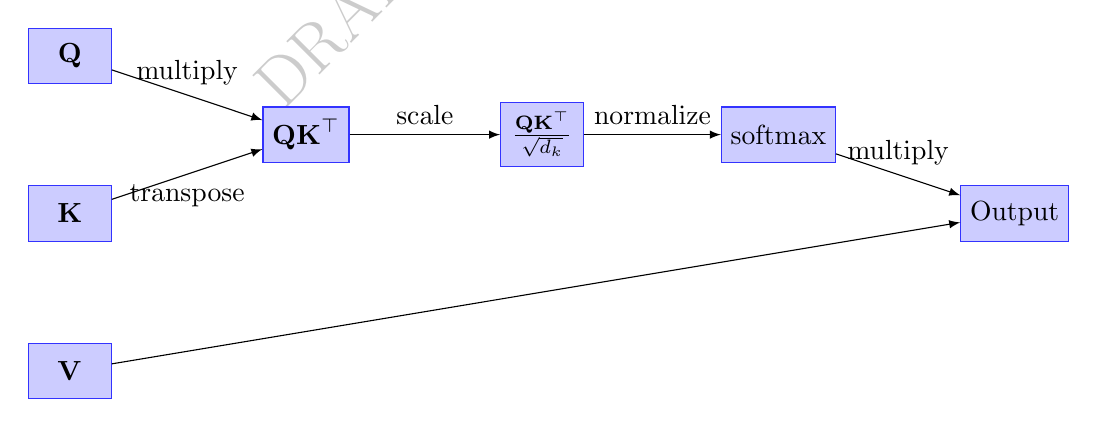
\begin{tikzpicture}[
    node/.style={rectangle, draw=blue!80, fill=blue!20, minimum size=20pt},
    matrix/.style={node, minimum width=30pt},
    vector/.style={node, minimum width=20pt},
    >=latex
]
    % Input matrices
    \node[matrix] (Q) at (0,2) {$\mathbf{Q}$};
    \node[matrix] (K) at (0,0) {$\mathbf{K}$};
    \node[matrix] (V) at (0,-2) {$\mathbf{V}$};
    
    % Matrix multiplication
    \node[matrix] (QK) at (3,1) {$\mathbf{QK}^\top$};
    
    % Scaling
    \node[matrix] (scaled) at (6,1) {$\frac{\mathbf{QK}^\top}{\sqrt{d_k}}$};
    
    % Softmax
    \node[matrix] (softmax) at (9,1) {softmax};
    
    % Final multiplication
    \node[matrix] (output) at (12,0) {Output};
    
    % Arrows and labels
    \draw[->] (Q) -- node[above] {multiply} (QK);
    \draw[->] (K) -- node[below] {transpose} (QK);
    \draw[->] (QK) -- node[above] {scale} (scaled);
    \draw[->] (scaled) -- node[above] {normalize} (softmax);
    \draw[->] (softmax) -- node[above] {multiply} (output);
    \draw[->] (V) -- (output);
\end{tikzpicture}
\caption{Scaled Dot-Product Attention Mechanism: The process transforms query ($\mathbf{Q}$), key ($\mathbf{K}$), and value ($\mathbf{V}$) matrices into attention-weighted outputs through matrix multiplication, scaling, and softmax normalization.}
\label{fig:attention_mechanism}
\end{figure}

\noindent
The \textbf{self-attention} mechanism is a key innovation of the Transformer architecture that allows a model to focus on different parts of a sequence when processing a given token. Unlike recurrent models, which rely on hidden states passed along sequentially, self-attention provides a global view of the entire sequence at each time step.

\subsection{Query, Key, and Value Formulation}
\noindent
In self-attention, each token in a sequence is first mapped to three different vectors:
\begin{itemize}
    \item A \textbf{Query} vector $\mathbf{q}_i$ - represents what the current token is "looking for"
    \item A \textbf{Key} vector $\mathbf{k}_i$ - represents what the token can "match against"
    \item A \textbf{Value} vector $\mathbf{v}_i$ - represents the actual content to be aggregated
\end{itemize}
These vectors are obtained through learned linear transformations of the input embeddings:
\begin{align*}
    \mathbf{Q} &= \mathbf{X}\mathbf{W}^Q \\
    \mathbf{K} &= \mathbf{X}\mathbf{W}^K \\
    \mathbf{V} &= \mathbf{X}\mathbf{W}^V
\end{align*}
where $\mathbf{X}$ is the input sequence and $\mathbf{W}^Q, \mathbf{W}^K, \mathbf{W}^V$ are learnable parameter matrices.

\subsection{Scaled Dot-Product Attention}
\noindent
The attention mechanism computes a weighted sum of values, where the weights are determined by the compatibility between queries and keys. The complete formula is:
\[
\text{Attention}(\mathbf{Q}, \mathbf{K}, \mathbf{V}) 
= \text{softmax}\!\Bigl(\frac{\mathbf{Q} \mathbf{K}^\top}{\sqrt{d_k}}\Bigr) \mathbf{V}
\]

The computation proceeds in four steps (as illustrated in Figure \ref{fig:attention_mechanism}):
\begin{enumerate}
    \item \textbf{Compatibility Scores:} Compute $\mathbf{Q}\mathbf{K}^\top$ to get raw attention scores
    \item \textbf{Scaling:} Divide by $\sqrt{d_k}$ to prevent extremely large values in high dimensions
    \item \textbf{Softmax:} Apply softmax to get a probability distribution over all positions
    \item \textbf{Value Aggregation:} Multiply with $\mathbf{V}$ to get the final attention-weighted output
\end{enumerate}

\subsection{The Importance of Scaling}
\noindent
The scaling factor $\sqrt{d_k}$ is crucial for stable training because:
\begin{itemize}
    \item As dimension $d_k$ increases, dot products grow larger in magnitude
    \item Large values lead to extremely small gradients in the softmax
    \item Scaling keeps the values in a reasonable range where gradients flow well
\end{itemize}

This is related to the concept of softmax temperature $\tau$, where:
\[
\text{softmax}\bigl(\frac{\mathbf{Q}\mathbf{K}^\top}{\sqrt{d_k} \,\tau}\bigr)
\]
controls how "sharp" or "soft" the attention distribution becomes.

\subsection{Masked Self-Attention}
\noindent
For autoregressive tasks like language modeling, we need to ensure that predictions for position $i$ can only depend on positions $\leq i$. This is achieved through masked self-attention:
\[
\text{Attention}(\mathbf{Q}, \mathbf{K}, \mathbf{V}, \mathbf{M}) 
= \text{softmax}\!\Bigl(\frac{\mathbf{Q} \mathbf{K}^\top + \mathbf{M}}{\sqrt{d_k}}\Bigr) \mathbf{V}
\]
where $\mathbf{M}$ is a mask matrix with elements:
\[
M_{ij} = \begin{cases}
    0 & \text{if position } j \leq i \\
    -\infty & \text{otherwise}
\end{cases}
\]

\subsection{Computational Complexity}
\noindent
The self-attention mechanism has complexity characteristics that are important to consider:
\begin{itemize}
    \item Time Complexity: $O(n^2d_k)$ for sequence length $n$
    \item Memory Complexity: $O(n^2)$ for storing attention weights
    \item Parallelization: Highly parallelizable across all positions
\end{itemize}

This quadratic complexity in sequence length has led to various efficient attention variants for handling long sequences, but the basic mechanism remains central to modern LLMs.

% Attention mechanism formula
\begin{equation}\label{eq:attention_mechanism}
\text{Attention}(\mathbf{Q}, \mathbf{K}, \mathbf{V}) = \text{softmax}\!\Bigl(\frac{\mathbf{Q}\mathbf{K}^\top}{\sqrt{d_k}}\Bigr)\mathbf{V}
\end{equation}

% Masked attention
\begin{equation}\label{eq:masked_attention}
\text{Attention}(\mathbf{Q}, \mathbf{K}, \mathbf{V}, \mathbf{M}) 
= \text{softmax}\!\Bigl(\frac{\mathbf{Q} \mathbf{K}^\top + \mathbf{M}}{\sqrt{d_k}}\Bigr) \mathbf{V}
\end{equation}

% Mask matrix definition
\begin{equation}\label{eq:mask_matrix}
M_{ij} = \begin{cases}
    0 & \text{if position } j \leq i \\
    -\infty & \text{otherwise}
\end{cases}
\end{equation}

\section{Multi-Head Attention}\index{attention!multi-head}\index{multi-head attention}
\label{sec:multi_head_attention}
% PROMPT: Provide a small example demonstrating multi-head attention outputs

\noindent
Multi-head attention\index{multi-head attention!definition}~\cite{vaswani2017attention,devlin2018bert} extends single-head attention by running multiple attention mechanisms in parallel. Each head can specialize in different aspects of the input, allowing the model to jointly attend to information from different representation subspaces\index{representation subspaces} at different positions.

\subsection{Motivation and Intuition}\index{multi-head attention!motivation}
\noindent
The key insight behind multi-head attention lies in its ability to capture diverse relationships between tokens simultaneously. Through specialized pattern recognition\index{pattern recognition}, different heads learn to focus on distinct aspects of the input. Some heads may specialize in syntactic relationships like subject-verb agreement, while others focus on semantic connections between synonyms and antonyms. Certain heads become adept at coreference resolution, tracking pronouns and their antecedents, while others might concentrate on entity relationships between people, places, and organizations.

The parallel processing nature\index{parallel processing} of multi-head attention provides several computational advantages. By maintaining multiple views of the same input, the model can learn different patterns independently. This parallel architecture not only enables efficient computation but also provides ensemble-like benefits from the multiple heads working in concert.

\subsection{Architectural Details}\index{multi-head attention!architecture}
\noindent
The multi-head attention mechanism processes queries, keys, and values through multiple parallel heads with careful parameter organization\index{parameter matrices}. Each attention head possesses its own learned projections, with separate transformations for queries, keys, and values. These individual projections are combined through a final output projection that integrates information from all heads. The dimensionality is carefully balanced across heads to maintain computational efficiency while maximizing representational power.

The attention computation\index{attention computation} occurs in parallel across all heads, with each head performing its own scaled dot-product attention operation. This parallel structure allows different heads to develop independent attention patterns, capturing various aspects of the input relationships. The results from all heads are then concatenated and projected to produce the final output.

\subsection{Head Specialization}\index{head specialization}
\noindent
Research has revealed distinct patterns of specialization across different attention heads. \textbf{Syntactic heads}\index{syntactic heads} focus on grammatical structure, handling subject-verb dependencies, prepositional phrase attachments, clause boundaries, and part-of-speech patterns. Meanwhile, \textbf{semantic heads}\index{semantic heads} concentrate on meaning-based relationships, managing entity tracking, topic focus, semantic similarity, and contextual disambiguation. Additionally, \textbf{positional heads}\index{positional heads} specialize in spatial relationships, addressing local context attention, long-range dependencies, relative position encoding, and boundary detection.

\subsection{Implementation Considerations}\index{multi-head attention!implementation}
\noindent
Several practical aspects significantly influence implementation and performance. The \textbf{number of heads}\index{number of heads} represents a crucial trade-off between expressiveness and computational efficiency. While typical values range from 8 to 32, the optimal number often scales with model size. However, there are diminishing returns beyond certain points. The \textbf{head dimension}\index{head dimension} must balance computation and representation power, typically achieved by dividing the total dimension by the number of heads. This choice impacts both memory usage and computation time, with important implications for model depth.

\textbf{Attention dropout}\index{attention dropout} plays a vital role in regularization. Applied to attention weights, it prevents over-reliance on specific heads and improves generalization. Different dropout rates may be employed across different layers, allowing for fine-tuned regularization throughout the network.

\subsection{Advanced Variations}\index{multi-head attention!variations}
\noindent
Recent research has introduced several sophisticated improvements to the basic architecture. \textbf{Sparse attention}\index{sparse attention} mechanisms reduce computation through structured sparsity, implementing local-global attention patterns and adaptive sparsity based on content. These approaches often employ efficient implementation strategies to maximize performance gains.

\textbf{Grouped attention}\index{grouped attention} explores parameter sharing between related heads, implementing hierarchical attention structures and dynamic head grouping. This approach can significantly reduce parameter count while maintaining model capacity. \textbf{Adaptive mechanisms}\index{adaptive mechanisms} take this further by introducing dynamic pruning of attention heads, task-specific head selection, conditional computation, and attention head ensembling.

\subsection{Impact on Model Performance}\index{multi-head attention!performance impact}
\noindent
Multi-head attention enhances model performance through several key mechanisms. The \textbf{improved representation}\index{representation improvement} capability enables richer feature capture and better handling of ambiguity, leading to enhanced contextual understanding and more robust embeddings. The architecture's influence on \textbf{training dynamics}\index{training dynamics} manifests in faster convergence and more stable gradients, resulting in better optimization properties and reduced vanishing gradient problems.

The multi-head design also contributes to \textbf{model robustness}\index{model robustness} through redundancy across heads, enabling better generalization and increased fault tolerance. This architectural choice has proven particularly valuable for improving out-of-distribution performance.

% Add relevant citations
\nocite{michel2019sixteen, voita2019analyzing, raganato2018analysis}

\subsection{Splitting and Recombining Embeddings}\index{embeddings!splitting}\index{embeddings!recombining}
Suppose each token in a sequence is represented by an embedding of dimension $d_\text{model}$\index{embedding!dimension}. In a multi-head attention layer with $h$ heads\index{attention!number of heads}, we split the embedding into $h$ smaller segments\index{embedding!segments}, each of dimension $d_k = d_\text{model} / h$\index{dimension!per head}. For each head:
\begin{enumerate}
    \item Compute its own \textbf{query} ($\mathbf{Q}$)\index{query matrix}, \textbf{key} ($\mathbf{K}$)\index{key matrix}, and \textbf{value} ($\mathbf{V}$)\index{value matrix} transformations, each of dimension $d_k$.
    \item Perform scaled dot-product attention\index{attention!scaled dot-product} using these smaller matrices.
    \item Obtain an attention output\index{attention!output} of dimension $d_k$.
\end{enumerate}
After all $h$ heads have computed their respective attention outputs, these outputs are concatenated\index{concatenation} and passed through a final linear projection\index{linear projection} back to dimension $d_\text{model}$. This process allows each head to learn a distinct way of attending to the tokens\index{attention patterns}.

\subsection{Benefits of Multiple Attention Heads}\index{multi-head attention!benefits}
\noindent
The parallel operation of attention across multiple subspaces yields substantial advantages for sequence processing. The enhanced representational power allows each head to specialize in capturing different types of dependencies\index{dependencies}, whether syntactic\index{syntactic dependencies}, semantic\index{semantic dependencies}, or positional\index{positional cues}. This multi-head architecture provides natural redundancy and robustness\index{redundancy}\index{robustness}, ensuring that even if some heads fail to learn useful representations\index{representations!useful}, others can compensate. Furthermore, splitting the embedding space improves gradient flow\index{gradient flow} by lowering the dimensionality\index{dimensionality} of each attention computation, which helps stabilize gradients\index{gradient stability} and accelerate training\index{training speed}.

\subsection{Mathematical Notation for Multi-Head Attention}\index{multi-head attention!mathematical notation}
\noindent
Let $\mathbf{X} \in \mathbb{R}^{n \times d_\text{model}}$ be the matrix of input embeddings\index{input embeddings} (one token per row). For each head $i \in \{1, \ldots, h\}$, define parameter matrices\index{parameter matrices}:
\[
\mathbf{W}_\mathbf{Q}^{(i)} \in \mathbb{R}^{d_\text{model} \times d_k}, \quad
\mathbf{W}_\mathbf{K}^{(i)} \in \mathbb{R}^{d_\text{model} \times d_k}, \quad
\mathbf{W}_\mathbf{V}^{(i)} \in \mathbb{R}^{d_\text{model} \times d_k}.
\]
The output of head $i$ is:
\[
\text{head}_i(\mathbf{X}) = \text{Attention}\!\Bigl(\mathbf{X}\mathbf{W}_\mathbf{Q}^{(i)},\, \mathbf{X}\mathbf{W}_\mathbf{K}^{(i)},\, \mathbf{X}\mathbf{W}_\mathbf{V}^{(i)}\Bigr).
\]
After computing all $h$ heads, we concatenate their outputs along the feature dimension\index{feature dimension}:
\[
\text{Concat}(\text{head}_1, \ldots, \text{head}_h) \in \mathbb{R}^{n \times (h \cdot d_k)}.
\]
Finally, this concatenated vector is projected back to $d_\text{model}$ using a linear transformation $\mathbf{W}_O$\index{output projection}:
\[
\text{MultiHead}(\mathbf{X}) 
= \text{Concat}(\text{head}_1, \ldots, \text{head}_h)\,\mathbf{W}_O.
\]
\noindent
Here, $\mathbf{W}_O \in \mathbb{R}^{(h \cdot d_k) \times d_\text{model}}$ combines information from each attention head into the final output dimension. This design fosters multiple perspectives on the input sequence—often resulting in more nuanced and powerful contextual representations.

\begin{pythoncode}[Multi-Head Attention Implementation]
class MultiHeadAttention(nn.Module):
    def __init__(self, d_model, num_heads):
        """
        Initialize multi-head attention module
        Args:
            d_model: Model dimension (total embedding size)
            num_heads: Number of attention heads
        """
        super().__init__()
        self.d_model = d_model
        self.num_heads = num_heads
        self.d_k = d_model // num_heads  # Dimension per head
        
        # Linear projections for Q, K, V for all heads, for all i
        self.W_q = nn.Linear(d_model, d_model)  # W_Q^(i)
        self.W_k = nn.Linear(d_model, d_model)  # W_K^(i)
        self.W_v = nn.Linear(d_model, d_model)  # W_V^(i)
        
        # Final output projection
        # W_O from equation \ref{eq:multihead_final}
        self.W_o = nn.Linear(d_model, d_model)  
    
    def forward(self, x, mask=None):
        batch_size = x.size(0)
        
        # Linear projections and reshape for multiple heads
        # Split d_model into num_heads * d_k as in equation \ref{eq:mha_params}
        q = self.W_q(x).view(batch_size, -1, self.num_heads, self.d_k).transpose(1, 2)
        k = self.W_k(x).view(batch_size, -1, self.num_heads, self.d_k).transpose(1, 2)
        v = self.W_v(x).view(batch_size, -1, self.num_heads, self.d_k).transpose(1, 2)
        
        # Compute attention for each head 
        scores = torch.matmul(q, k.transpose(-2, -1)) / math.sqrt(self.d_k)
        if mask is not None:
            scores = scores.masked_fill(mask == 0, float('-inf'))
        attention_weights = F.softmax(scores, dim=-1)
        
        # Apply attention weights to values
        head_outputs = torch.matmul(attention_weights, v)
        
        # Concatenate and project back to d_model dimensions        
        output = head_outputs.transpose(1, 2).contiguous() \\
                 .view(batch_size, -1, self.d_model)
        return self.W_o(output)
\end{pythoncode}

\noindent
As we will see, multi-head attention serves as a fundamental building block not only in the encoder and decoder components but also in the cross-attention mechanisms that bridge these elements together. Recent work has further refined these concepts through efficient variants like sparse attention~\cite{fedus2021switch} and optimized implementations~\cite{dao2022flashattention}.

% Parameter matrices dimensions
\begin{equation}\label{eq:mha_params}
\mathbf{W}_\mathbf{Q}^{(i)} \in \mathbb{R}^{d_\text{model} \times d_k}, \quad
\mathbf{W}_\mathbf{K}^{(i)} \in \mathbb{R}^{d_\text{model} \times d_k}, \quad
\mathbf{W}_\mathbf{V}^{(i)} \in \mathbb{R}^{d_\text{model} \times d_k}
\end{equation}

% Single head output
\begin{equation}\label{eq:single_head}
\text{head}_i(\mathbf{X}) = \text{Attention}\!\Bigl(\mathbf{X}\mathbf{W}_\mathbf{Q}^{(i)},\, \mathbf{X}\mathbf{W}_\mathbf{K}^{(i)},\, \mathbf{X}\mathbf{W}_\mathbf{V}^{(i)}\Bigr)
\end{equation}

% Concatenation
\begin{equation}\label{eq:head_concat}
\text{Concat}(\text{head}_1, \ldots, \text{head}_h) \in \mathbb{R}^{n \times (h \cdot d_k)}
\end{equation}

% Final multi-head output
\begin{equation}\label{eq:multihead_final}
\text{MultiHead}(\mathbf{X}) 
= \text{Concat}(\text{head}_1, \ldots, \text{head}_h)\,\mathbf{W}_O
\end{equation} 

Recent work has explored efficient variants like sparse attention~\cite{fedus2021switch} and optimized implementations~\cite{dao2022flashattention}.



\chapter{Transformer Encoder-Decoder Structure}
\label{chap:transformer_structure}

\noindent
The encoder-decoder architecture represents a powerful paradigm for transforming one sequence into another. Think of it as a two-stage process:

\begin{itemize}
    \item \textbf{The Encoder} acts like a sophisticated reader, processing the input sequence (e.g., a French sentence) and creating a rich, contextual understanding of it. Each input token gets updated to reflect its relationships with all other tokens in the sequence.
    
    \item \textbf{The Decoder} acts as a skilled writer, generating the output sequence (e.g., an English translation) one token at a time. At each step, it:
    \begin{itemize}
        \item Looks at what it has generated so far (self-attention)
        \item Consults the encoder's understanding of the input (cross-attention)
        \item Decides what token to generate next
    \end{itemize}
\end{itemize}

\noindent
This separation of "understanding" and "generation" tasks allows the model to:
\begin{itemize}
    \item Capture complex relationships in the input (encoder)
    \item Maintain coherence in the output (decoder)
    \item Create flexible mappings between input and output sequences
\end{itemize}

\noindent
Building upon attention, the Transformer architecture implements this encoder-decoder framework efficiently. This chapter explores how positional encodings, residual connections, and normalization layers come together in both encoder and decoder blocks. By the end, you will see how all these components integrate mathematically to form the backbone of modern LLMs.

\section{Positional Encodings}
\label{sec:positional_encodings}
% PROMPT: Compare sinusoidal to learned positional embeddings

\noindent
Transformers dispense with the notion of sequence order imposed by recurrent or convolutional architectures, requiring an explicit way to inject positional information into token embeddings. \textbf{Positional encodings} achieve this by adding (or concatenating) position-dependent vectors to the input embeddings, enabling the model to distinguish the order of tokens. Below, we delve into the common \textbf{sinusoidal} approach and briefly discuss some alternative methods.

\subsection{Sinusoidal Positional Embeddings: The Math Behind Them}
\noindent
In the original Transformer architecture, each position $pos$ in the input sequence is mapped to a \emph{sinusoidal} embedding vector of dimension $d_\text{model}$. For each dimension $i \in \{0, \ldots, d_\text{model}-1\}$, the encoding is defined as:
\[
\begin{aligned}
\text{PE}(pos, 2i) &= \sin\Bigl(pos \cdot 10000^{-\frac{2i}{d_\text{model}}}\Bigr), \\[6pt]
\text{PE}(pos, 2i+1) &= \cos\Bigl(pos \cdot 10000^{-\frac{2i}{d_\text{model}}}\Bigr).
\end{aligned}
\]
\begin{itemize}
    \item \textbf{Variable Frequency.} The factor $10000^{-\frac{2i}{d_\text{model}}}$ sets different frequencies for each dimension. Lower dimensions vary more slowly with respect to $pos$, while higher dimensions vary more quickly.
    \item \textbf{Relative Distance.} The combination of sines and cosines at varying frequencies allows the model to easily compute relative distances between positions, since shifting $pos$ by a fixed amount produces predictable phase shifts in these trigonometric functions.
    \item \textbf{Implementation.} During training, these positional vectors are added to (or concatenated with) the token embeddings before being passed to the first Transformer layer.
\end{itemize}

\noindent
\textbf{Why Sines and Cosines?} Beyond their periodic nature, sine and cosine functions ensure that positions far outside the training range still produce valid embeddings—unlike learned positional vectors that might not generalize to sequence lengths unseen during training.

\subsection{Alternative Positional Encoding Methods}
\noindent
While sinusoidal encodings are conceptually elegant, multiple alternatives have emerged to address various use cases:

\textbf{Learned Positional Embeddings}\index{positional embeddings!learned} assign a trainable vector to each possible position index. This approach can sometimes improve performance on in-distribution sequence lengths but may generalize poorly to longer sequences than seen in training.

\textbf{Relative Position Representations}\index{positional embeddings!relative} focus on how tokens relate to each other's positions rather than absolute indices. This approach often leads to better handling of long sequences and repetitive patterns, particularly in models like BERT or T5.

\textbf{Rotary Positional Embeddings (RoPE)}\index{positional embeddings!rotary} rotate query and key vectors in a complex plane according to their positions, potentially improving how attention scales with longer contexts. This method has gained traction in some large language models for better long-sequence extrapolation.

\textbf{Mixtures of Encodings}\index{positional embeddings!hybrid} combine different forms of positional encoding—e.g., adding a learned component on top of a sinusoidal base—to strike a balance between generalization and flexibility.

\noindent
No single encoding method universally dominates; choice often depends on the target domain (e.g., natural language vs. code), desired sequence lengths, and computational constraints. Regardless of the specific approach, \textbf{positional encodings} remain a critical design component, ensuring that Transformers can accurately model the order and structure of sequential data.

\section{Encoder Block}
\label{sec:encoder_block}
% PROMPT: Expand on the role of layer normalization

\noindent
The Transformer encoder consists of alternating layers of multi-head self-attention and position-wise feedforward networks...

\noindent
A Transformer \textbf{encoder block} is a modular building unit consisting of two main sub-layers: multi-head self-attention and a position-wise feedforward network. Each sub-layer is wrapped with additional operations (residual connections and layer normalization) to stabilize and improve training. This section focuses on two crucial components in this architecture: \textbf{layer normalization} and \textbf{residual connections}.

\subsection{Layer Normalization and Its Role in Stable Training}
\noindent
\textbf{Layer normalization} (LayerNorm) is applied to the intermediate representations to stabilize the distribution of activations. Unlike batch normalization, which computes statistics across a batch dimension, layer normalization computes statistics \emph{across the feature dimension} for each training example:
\begin{equation}
\begin{aligned}
\text{LayerNorm}(\mathbf{x}) &= \frac{\mathbf{x} - \mu(\mathbf{x})}{\sigma(\mathbf{x})} \cdot \boldsymbol{\gamma} + \boldsymbol{\beta},
\end{aligned}
\end{equation}
where:
\begin{itemize}
    \item $\mu(\mathbf{x})$ is the mean of the features in $\mathbf{x}$,
    \item $\sigma(\mathbf{x})$ is the standard deviation,
    \item $\boldsymbol{\gamma}$ and $\boldsymbol{\beta}$ are learnable parameters that allow the network to rescale and shift the normalized output back to a suitable range.
\end{itemize}

\noindent
\textbf{Key Benefits of LayerNorm for Transformers:}
\begin{itemize}
    \item \textbf{Stability During Training.} Normalizing each activation vector by its own mean and variance reduces the risk of exploding or vanishing gradients, facilitating more reliable training across large parameter spaces.
    \item \textbf{Permutation Invariance.} Since layer normalization is applied to each token embedding \emph{individually}, it remains effective for variable batch sizes and sequence lengths.
    \item \textbf{Reduced Internal Covariate Shift.} By standardizing activations, the model learns more robustly across layers, ensuring that updates in one part of the network do not excessively disrupt the distribution of inputs to another part.
\end{itemize}

\subsection{Residual Connections: Rationale and Benefits}
\noindent
Transformers rely heavily on \textbf{residual connections} (also known as skip connections) to simplify gradient flow and enable deeper architectures. In each sub-layer, we add a skip connection from the input of the sub-layer to its output:
\begin{equation}
\begin{aligned}
\mathbf{z} &= \text{LayerNorm}\Bigl(\mathbf{x} + \text{SubLayer}(\mathbf{x})\Bigr),
\end{aligned}
\end{equation}
where $\mathbf{x}$ is the input to the sub-layer, and $\mathbf{z}$ is the final output of that sub-layer (after layer normalization).

\begin{itemize}
    \item \textbf{Improved Gradient Propagation.} The skip connection provides a path for gradients to flow from deeper layers back to earlier ones, mitigating the vanishing gradient problem and accelerating convergence.
    \item \textbf{Better Convergence at Scale.} Residual connections help maintain stable activations when training very deep models or very large models—common in modern LLMs.
    \item \textbf{Identity Function as a Baseline.} If the sub-layer fails to learn anything useful, the output can revert to the input via the identity mapping, preventing severe performance degradation.
\end{itemize}

\noindent
In practice, each encoder block is composed of:
\begin{equation}\label{eq:encoder_block}
\begin{aligned}
\text{EncoderBlock}(\mathbf{x}) &= \text{LayerNorm}\Bigl(\mathbf{x} + \text{MultiHeadSelfAttn}(\mathbf{x})\Bigr) \\
&\rightarrow \text{LayerNorm}\Bigl(\mathbf{z} + \text{FFN}(\mathbf{z})\Bigr)
\end{aligned}
\end{equation}
where $\mathbf{z}$ is the intermediate output after the self-attention step. Repeated stacking of these encoder blocks enables hierarchical abstraction of the input sequence representations.


\section{Decoder Block}
\label{sec:decoder_block}
% PROMPT: Clarify the difference between encoder self-attention and decoder self-attention

\noindent
The \textbf{decoder block} in a Transformer is similarly structured to the encoder block but includes additional mechanisms crucial for auto-regressive generation. Specifically, the decoder block features~\cite{liu2019roberta}:
\begin{enumerate}
    \item \textbf{Masked Multi-Head Self-Attention}
    \item \textbf{Encoder-Decoder Cross-Attention}
    \item \textbf{Position-Wise Feedforward Network}
\end{enumerate}
Layer normalization and residual connections are also applied, just as in the encoder.

\subsection{Masked Multi-Head Attention}
\noindent
In the decoder, the \emph{self-attention} sub-layer is \textbf{masked} to preserve causality in language generation tasks. This means each token can only attend to itself and the \emph{previous} tokens in the sequence. Formally,
\[
\text{Attention}(\mathbf{Q}, \mathbf{K}, \mathbf{V}, \mathbf{M}) 
= \text{softmax}\Bigl(\frac{\mathbf{Q}\mathbf{K}^\top + \mathbf{M}}{\sqrt{d_k}}\Bigr)\mathbf{V},
\]
where $\mathbf{M}$ is a mask matrix that sets attention scores to $-\infty$ for positions representing future tokens.

\subsection{Encoder-Decoder Cross-Attention}
\noindent
Unlike the encoder, the decoder also needs to incorporate the representations learned by the encoder. The \textbf{encoder-decoder cross-attention} sub-layer accomplishes this:
\[
\text{CrossAttention}(\mathbf{Q}, \mathbf{K}, \mathbf{V}) 
= \text{softmax}\Bigl(\frac{\mathbf{Q}\mathbf{K}^\top}{\sqrt{d_k}}\Bigr)\mathbf{V},
\]
where now
\begin{itemize}
    \item $\mathbf{Q}$ comes from the \emph{decoder} hidden states,
    \item $\mathbf{K}, \mathbf{V}$ come from the final \emph{encoder} outputs.
\end{itemize}
This step allows the decoder to focus on relevant information from the entire source sequence during generation.

\subsection{Combining Outputs for Language Generation}
\noindent
Following self-attention and cross-attention, the \textbf{position-wise feedforward network} (FFN) is applied. As with the encoder, each sub-layer is surrounded by residual connections and layer normalization. The output of the decoder block is then passed to the next decoder block or ultimately used to predict the next token in auto-regressive fashion.

\begin{equation}\label{eq:decoder_block}
\text{DecoderBlock}(\mathbf{y}) = 
\text{LayerNorm}\Bigl(\mathbf{y} + \text{MaskedSelfAttn}(\mathbf{y})\Bigr)
\rightarrow
\text{LayerNorm}\Bigl(\mathbf{z} + \text{CrossAttn}(\mathbf{z}, \mathbf{x}_{\text{enc}})\Bigr)
\rightarrow
\text{LayerNorm}\Bigl(\mathbf{w} + \text{FFN}(\mathbf{w})\Bigr)
\end{equation}
where $\mathbf{y}$ is the decoder input (shifted right tokens), $\mathbf{x}_{\text{enc}}$ represents the encoder outputs, and $\mathbf{z}$, $\mathbf{w}$ are intermediate states.

\noindent
This process is repeated for each token in the output sequence (e.g., each time step in auto-regressive generation). The distinction between \emph{encoder self-attention} (bidirectional, unmasked) and \emph{decoder self-attention} (unidirectional, masked) ensures that the model does not peek at future tokens—preserving the causal property necessary for language generation.


\section{Mathematical Notation of the Transformer}
\label{sec:transformer_notation}
% PROMPT: Collect all the main formulas for easy reference

\noindent
The Transformer's power lies in its ability to process sequences in a fully parallel manner while preserving context via self-attention. Below is a concise reference to the core formulas that define the encoder-decoder structure, highlighting \textbf{layer norms}, \textbf{attention mechanisms}, and the \textbf{feedforward} layers.

\subsection{Attention Mechanisms}
\begin{align}
&\textbf{Scaled Dot-Product Attention:}\notag\\
&\quad \text{Attention}(\mathbf{Q}, \mathbf{K}, \mathbf{V}) 
= \text{softmax}\!\Bigl(\frac{\mathbf{Q} \mathbf{K}^\top}{\sqrt{d_k}}\Bigr) \mathbf{V}. \label{eq:attention} \\[6pt]
&\textbf{Multi-Head Attention (MHA):}\notag\\
&\quad
\text{head}_i(\mathbf{X}) 
= 
\text{Attention}\Bigl(
\mathbf{X}\mathbf{W}_\mathbf{Q}^{(i)},\ 
\mathbf{X}\mathbf{W}_\mathbf{K}^{(i)},\ 
\mathbf{X}\mathbf{W}_\mathbf{V}^{(i)}
\Bigr), \label{eq:mha_head} \\
&\quad 
\text{MHA}(\mathbf{X}) 
= 
\text{Concat}(\text{head}_1, \ldots, \text{head}_h)\,\mathbf{W}_O. \label{eq:mha_final}
\end{align}

\subsection{Layer Normalization and Residual Connections}
\begin{align*}
&\mathbf{z} = \text{LayerNorm}\Bigl(\mathbf{x} + \text{SubLayer}(\mathbf{x})\Bigr), \\
&\text{where} \quad
\text{LayerNorm}(\mathbf{x}) 
= 
\frac{\mathbf{x} - \mu(\mathbf{x})}{\sigma(\mathbf{x})} \cdot \boldsymbol{\gamma} + \boldsymbol{\beta}.
\end{align*}
Here, $\mu(\mathbf{x})$ and $\sigma(\mathbf{x})$ denote the mean and standard deviation computed over the feature dimension of $\mathbf{x}$, respectively.

\subsection{Feedforward Networks (FFN)}
\begin{align*}
&\text{FFN}(\mathbf{x}) = \max(0, \mathbf{x}\mathbf{W}_1 + \mathbf{b}_1)\,\mathbf{W}_2 + \mathbf{b}_2,
\end{align*}
often with ReLU or GELU activation in the middle layer. The parameters $\mathbf{W}_1, \mathbf{W}_2, \mathbf{b}_1, \mathbf{b}_2$ are shared across positions but differ from one layer to another.

\subsection{Putting It All Together}
\noindent
An \textbf{encoder layer} comprises:
\[
\mathbf{z} = \text{LayerNorm}\Bigl(\mathbf{x} + \text{MHA}(\mathbf{x})\Bigr), \quad
\mathbf{z}' = \text{LayerNorm}\Bigl(\mathbf{z} + \text{FFN}(\mathbf{z})\Bigr).
\]
Multiple encoder layers are stacked to form the entire encoder module.

\noindent
A \textbf{decoder layer} includes:
\[
\mathbf{y}' = \text{LayerNorm}\Bigl(\mathbf{y} + \text{MaskedMHA}(\mathbf{y})\Bigr),\quad
\mathbf{y}'' = \text{LayerNorm}\Bigl(\mathbf{y}' + \text{CrossAttn}(\mathbf{y}', \mathbf{x}_{\text{enc}})\Bigr),
\]
\[
\mathbf{y}''' = \text{LayerNorm}\Bigl(\mathbf{y}'' + \text{FFN}(\mathbf{y}'')\Bigr).
\]
The final decoder output is typically fed into a projection layer to produce logits over the vocabulary for next-token prediction.

\noindent
These formulas encapsulate the core mathematical framework of the Transformer. Subtle variations exist across different implementations (e.g., pre-layer normalization vs. post-layer normalization), but the core operations—\emph{multi-head attention, residual connections, feedforward networks, and normalization}—remain consistent. By internalizing these operations, one can more deeply understand how modern LLMs process large-scale textual data and generate coherent, context-aware responses.


\chapter{The Transformer: A Walkthrough}\index{transformer!walkthrough}\index{architecture!transformer}

\begin{figure}[h]
\begin{center}
    \includegraphics[width=0.8\textwidth]{images/transformer_arch.png}
    \captionof{figure}{The Transformer Architecture}
    \end{center}
\end{figure}

\section{Introduction}
\noindent
Having explored the individual components of the Transformer in previous chapters, we now examine how these elements work together to process sequences effectively. The architecture's power comes not just from its individual innovations, but from their careful integration into a cohesive system\index{transformer!system integration}.

\section{Information Flow in the Transformer}\index{transformer!information flow}
\noindent
The Transformer processes information through a carefully orchestrated sequence of operations\index{sequence processing}. The journey begins with input processing\index{input processing}, where raw text is first tokenized into discrete indices\index{tokenization}, then mapped to dense vectors through token embeddings\index{token embeddings}. These embeddings are augmented with positional encodings\index{positional encodings} (discussed in Section~\ref{sec:positional_encodings}) to preserve sequence order information\index{sequence order}, since the model processes all tokens in parallel\index{parallel processing}.

The encoder\index{encoder} then processes these enriched representations through multiple parallel blocks\index{encoder blocks}. Within each block, self-attention mechanisms\index{self-attention} (Section~\ref{sec:self_attention}) enable each token to directly interact with every other token in the sequence\index{token interaction}. Multi-head attention\index{multi-head attention} (Section~\ref{sec:multi_head_attention}) allows the model to capture different types of relationships simultaneously\index{relationship capture}, while position-wise feed-forward networks\index{feed-forward networks} transform each token's representation independently.

The decoder\index{decoder} completes the processing pipeline by generating output tokens one at a time\index{token generation}. It employs masked self-attention\index{masked self-attention} to prevent looking at future tokens during generation\index{future masking}, maintaining the causal nature of the prediction task\index{causality}. Cross-attention mechanisms\index{cross-attention} connect the decoder to the encoder's outputs\index{encoder-decoder connection}, allowing the model to draw relevant information from the input sequence while generating each new token.

\section{Architectural Synergies}\index{architectural synergies}
\noindent
The Transformer's effectiveness stems from how its components complement each other\index{component interaction}. Self-attention and positional encodings work in concert\index{attention-position synergy}, with attention providing content-based interactions while positional information maintains awareness of sequence structure\index{sequence structure}. Together, they capture both semantic relationships\index{semantic relationships} and structural patterns\index{structural patterns} in the input.

Multi-head attention and feed-forward networks form another powerful partnership\index{attention-FFN synergy}. While attention heads capture diverse relationships between tokens\index{token relationships}, the FFN layers add crucial non-linearity\index{non-linearity} and position-specific processing\index{position-specific processing}. This combination enables both rich token interactions and sophisticated feature transformations\index{feature transformation}.

The architecture's deep structure\index{deep structure} is made possible by residual connections\index{residual connections} and layer normalization\index{layer normalization} working in tandem. Residual connections preserve access to low-level features\index{feature preservation} throughout the network, while layer normalization ensures stable activation distributions\index{activation stability}. This synergy enables the reliable training of deep models that can capture hierarchical patterns in language\index{hierarchical patterns}.

\section{The Complete Pipeline}\index{transformer!pipeline}
\noindent
The full processing pipeline begins with input embedding and positioning\index{input embedding}, where discrete tokens are mapped into a continuous vector space\index{vector space} and enriched with positional information. This representation enables the parallel processing that gives the Transformer its computational efficiency\index{computational efficiency}.

The encoder stack\index{encoder stack} then builds rich contextual representations\index{contextual representations} by repeatedly applying self-attention and feed-forward transformations. Each layer in the stack captures increasingly abstract relationships\index{abstract relationships}, while maintaining the original sequence length and bidirectional context\index{bidirectional context}.

In the decoder stack\index{decoder stack}, auto-regressive generation\index{auto-regressive generation} proceeds one token at a time, with each prediction building upon previous outputs while drawing relevant information from the encoder's representations through cross-attention mechanisms. The decoder maintains causality through masked attention\index{masked attention}, ensuring predictions are based only on previously generated tokens\index{token prediction}.

Finally, the output projection layer\index{output projection} maps the decoder's representations back to the vocabulary space\index{vocabulary space}, enabling token prediction while maintaining a proper probabilistic interpretation\index{probabilistic interpretation} of the model's outputs.

\section{Design Philosophy}\index{transformer!design philosophy}
\noindent
The Transformer's design reflects several key principles that revolutionized sequence processing\index{sequence processing principles}. At its core, the architecture replaces sequential processing with parallel attention mechanisms\index{parallel attention}, enabling efficient training and inference\index{efficient training}. It provides direct access between tokens\index{direct token access}, eliminating the need for information to flow through intermediate states as in RNNs\index{RNN comparison}.

The design emphasizes stable training\index{stable training} through careful use of normalization and residual connections, allowing the construction of deep networks that can capture complex language patterns\index{language patterns}. The separation of encoding and decoding functions provides modularity\index{architectural modularity}, enabling flexible adaptation to various tasks and architectures.

For detailed mathematical formulations of these components, refer to Section~\ref{sec:transformer_notation} in the encoder block chapter.

\section{Impact on Modern Architectures}\index{transformer!modern impact}
\noindent
The Transformer architecture has spawned numerous variants\index{transformer variants} that adapt its core principles to different tasks and constraints. Encoder-only models\index{encoder-only models} like BERT\index{BERT} focus on bidirectional understanding, making them particularly suited for tasks requiring deep analysis of input text. These models excel at classification\index{classification tasks}, understanding, and analysis tasks where bidirectional context is crucial.

Decoder-only models\index{decoder-only models}, exemplified by GPT\index{GPT}, emphasize autoregressive generation\index{autoregressive generation}. By simplifying the architecture to focus on the generative aspect, these models have proven especially effective for large-scale training\index{large-scale training} and text generation tasks\index{text generation}. Their streamlined design has enabled scaling to unprecedented model sizes\index{model scaling}.

Hybrid approaches\index{hybrid approaches} have emerged that combine Transformer elements with other architectural innovations\index{architectural innovations}. These variants often optimize for specific applications\index{application-specific optimization}, demonstrating the flexibility and adaptability of the core Transformer principles\index{transformer principles}. The success of these adaptations highlights the fundamental soundness of the original design choices\index{design choices}.

\section{Training}
The Transformer is trained using a teacher-forcing method, where the ground truth output sequence (shifted one position to the right) is fed as input to the decoder. The loss function is typically cross-entropy between the predicted output distribution and the true output word.

\section{Summary}

The Transformer architecture has had a profound impact on NLP and other fields. Its ability to model long-range dependencies and its parallelizable nature have made it a powerful tool for various sequence-to-sequence tasks. This chapter provided a detailed overview of the Transformer's components and their functions. While this is a complex model, understanding its inner workings is crucial for anyone working with state-of-the-art NLP and sequence modeling techniques. Future research continues to build upon this foundation, exploring new attention mechanisms, scaling laws, and applications beyond language.

\part{Training Large Language Models}
\chapter{Language Modeling and Pretraining Objectives}\index{language modeling}\index{pretraining objectives}
\label{chap:lm_pretraining}

\noindent
Language modeling\index{language modeling!definition} in NLP involves predicting or representing textual data in a way that captures statistical regularities\index{statistical regularities}, semantics\index{semantics}, and contextual relationships\index{contextual relationships} among tokens\index{tokens}. In modern LLMs\index{LLM|see {Large Language Model}}, language modeling objectives underpin pretraining\index{pretraining}, enabling models to learn general-purpose linguistic representations\index{linguistic representations} from large-scale corpora\index{corpora!large-scale}.

\section{Fundamentals of Language Modeling}\index{language modeling!fundamentals}
\label{sec:lm_fundamentals}

\subsection{Probabilistic Framework}\index{probabilistic framework}
\noindent
Language modeling fundamentally treats text as a probabilistic sequence. Given a sequence of tokens \((w_1, \ldots, w_t)\), the model learns to estimate:
\[
P(w_{t+1} \mid w_1, \ldots, w_t)
\]
This conditional probability distribution forms the basis for both understanding and generating text.

\begin{figure}[ht]
    \centering
    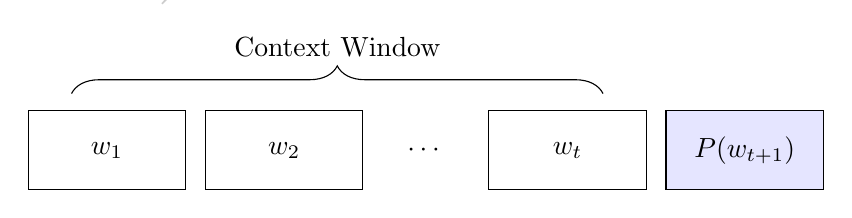
\begin{tikzpicture}[
        scale=0.9,
        token/.style={rectangle, draw, minimum width=2cm, minimum height=1cm},
        prob/.style={rectangle, draw, fill=blue!10, minimum width=2cm, minimum height=1cm}
    ]
        % Tokens
        \node[token] (w1) at (0,0) {$w_1$};
        \node[token] (w2) at (2.5,0) {$w_2$};
        \node (dots) at (4.5,0) {$\cdots$};
        \node[token] (wt) at (6.5,0) {$w_t$};
        \node[prob] (wt1) at (9,0) {$P(w_{t+1})$};
        
        % Arrows
        % \draw[-latex] (w1) -- (wt1);
        % \draw[-latex] (w2) -- (wt1);
        % \draw[-latex] (wt) -- (wt1);
        
        % Context window label
        \draw[decorate,decoration={brace,amplitude=10pt}] 
            (-0.5,0.8) -- (7,0.8) node[midway,above=10pt] {Context Window};
    \end{tikzpicture}
    \caption{Language modeling as next-token prediction. The model uses the context window to predict the probability distribution of the next token.}
    \label{fig:lm_prediction}
\end{figure}

\subsection{Vocabulary and Tokenization}\index{vocabulary}\index{tokenization}
\noindent
The choice of tokenization strategy significantly impacts model performance:

\begin{itemize}
    \item \textbf{Byte-Pair Encoding (BPE)}\index{BPE}: Iteratively merges frequent character pairs
    \item \textbf{WordPiece}\index{WordPiece}: Similar to BPE but uses likelihood instead of frequency
    \item \textbf{SentencePiece}\index{SentencePiece}: Language-agnostic tokenization
    \item \textbf{Unigram Language Model}\index{Unigram Language Model}: Probabilistic subword segmentation
\end{itemize}

\begin{figure}[ht]
    \centering
    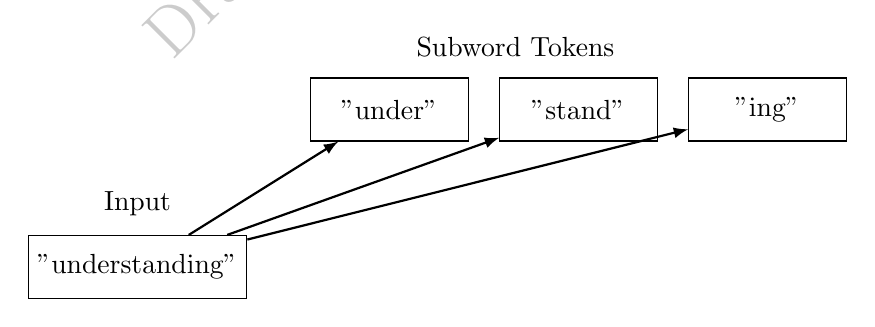
\begin{tikzpicture}[
        scale=0.8,
        box/.style={rectangle, draw, minimum width=2cm, minimum height=0.8cm},
        arrow/.style={-latex, thick}
    ]
        % Input text
        \node[box] (text) at (0,0) {"understanding"};
        
        % BPE tokens
        \node[box] (under) at (4,2.5) {"under"};
        \node[box] (stand) at (7,2.5) {"stand"};
        \node[box] (ing) at (10,2.5) {"ing"};
        
        % Arrows
        \draw[arrow] (text) -- (under);
        \draw[arrow] (text) -- (stand);
        \draw[arrow] (text) -- (ing);
        
        % Labels
        \node at (0,1) {Input};
        \node at (6,3.5) {Subword Tokens};
    \end{tikzpicture}
    \caption{Example of subword tokenization breaking down a word into constituent tokens.}
    \label{fig:tokenization}
\end{figure}

\section{Statistical Language Modeling}\index{statistical language modeling}
\label{sec:stat_lm}

\subsection{Maximum Likelihood Estimation (MLE) for Next-Token Prediction}\index{maximum likelihood estimation}\index{next-token prediction}
\noindent
A traditional approach to language modeling is to maximize the likelihood\index{likelihood maximization} of the observed sequence of tokens under the model's parameters\index{model parameters}. Given a training corpus of token sequences, we denote each sequence by \(\mathbf{w} = (w_1, w_2, \ldots, w_T)\). Under the \textbf{chain rule}\index{chain rule} of probability, the joint probability\index{joint probability} of the sequence is:
\[
P(\mathbf{w}) = \prod_{t=1}^{T} P(w_t \mid w_1, w_2, \ldots, w_{t-1}).
\]
To train the model, we often minimize the negative log-likelihood\index{negative log-likelihood} of the data:
\[
-\log P(\mathbf{w}) = -\sum_{t=1}^{T} \log P(w_t \mid w_1, \ldots, w_{t-1}),
\]
which is equivalent to maximizing \(P(\mathbf{w})\) under maximum likelihood estimation (MLE).

\subsection{Cross-Entropy Loss and Perplexity}\index{cross-entropy loss}\index{perplexity}
\noindent
In practice, we implement this via the \textbf{cross-entropy loss}\index{loss!cross-entropy}, commonly denoted as:
\[
\mathcal{L}_\text{CE} = -\sum_{t=1}^{T} \log \Bigl( P_{\theta}(w_t \mid w_1, \ldots, w_{t-1}) \Bigr),
\]
where \(P_{\theta}\) is the model distribution parameterized by \(\theta\). Cross-entropy compares the model's predicted distribution\index{predicted distribution} over tokens with the true one-hot distribution\index{one-hot distribution}, penalizing the model when it assigns low probability to the correct token.

\noindent
Two key metrics help us evaluate language model performance:

\textbf{Perplexity.}\index{perplexity!definition}
A common metric for language model performance\index{model performance}, \emph{perplexity} (PPL) is defined as:
\[
\text{PPL} = \exp\!\Bigl(\frac{1}{T}\sum_{t=1}^T -\log P_{\theta}(w_t \mid w_{<t})\Bigr).
\]
Conceptually, perplexity measures the average branching factor\index{branching factor} of the model's predictive distribution\index{predictive distribution}. A lower perplexity indicates that the model is less "surprised" by the data.

\textbf{Cross-Entropy vs. Perplexity.}\index{cross-entropy!vs perplexity}
While cross-entropy \(\mathcal{L}_\text{CE}\) is often used directly as the training objective, perplexity provides an intuitive, exponential-scale view of the model's uncertainty on test data.

\begin{figure}[ht]
    \centering
    \includegraphics[width=0.8\textwidth]{images/cross-entropy-perplexity.png}
    \caption{Typical training curves showing the relationship between cross-entropy loss and perplexity.}
    \label{fig:training_curves}
\end{figure}

\section{Masked Language Modeling (MLM)}\index{masked language modeling}
\label{sec:mlm}

\subsection{BERT-Style Masked Token Prediction}\index{BERT}\index{masked token prediction}
\noindent
\textbf{Masked Language Modeling (MLM)} is a pretraining objective popularized by BERT\index{BERT!masked language modeling}. In MLM, a certain percentage of tokens (e.g., 15\%) in a sequence are replaced by a special \texttt{[MASK]} token\index{mask token} or, less frequently, by random tokens\index{random tokens}. The model is then tasked with predicting the original tokens in these masked positions\index{masked positions}.

\begin{itemize}
    \item \textbf{Bidirectional Context.}\index{bidirectional context}
    Since the model can attend to tokens on both the left and right of a masked position, MLM captures bidirectional context more effectively than a strictly left-to-right approach\index{left-to-right approach}.
    \item \textbf{Robustness.}\index{robustness}
    By training to predict randomly masked tokens, the model learns more robust token representations\index{token representations}, reducing overfitting\index{overfitting} to specific sequential patterns\index{sequential patterns}.
\end{itemize}

\subsection{The Math Behind Partial Conditioning}
\noindent
For each masked position \(i\), the model's goal is to predict \(w_i\) given the remaining (unmasked) tokens:
\[
P(w_i \mid w_1, \ldots, \texttt{[MASK]}, \ldots, w_{j}, \ldots),
\]
where all but the masked tokens are visible. The loss is computed over just the masked positions, typically via a cross-entropy objective:
\[
\mathcal{L}_\text{MLM} = - \sum_{i \in M} \log P_{\theta}(w_i \mid \mathbf{w}_{\text{masked}}),
\]
where \(M\) is the set of masked indices. This \emph{partial conditioning} forces the network to infer the masked token using both left and right context, thus learning more powerful bidirectional representations.

\noindent
\textbf{Training Stability.}
Partial masking smooths the training signal by updating parameters based on a more varied set of contexts. The ability to predict one token given a surrounding window of unmasked tokens often leads to faster convergence and more robust representations.

\section{Causal Language Modeling (CLM)}\index{causal language modeling}
\label{sec:clm}

\subsection{GPT-Style Left-to-Right Prediction}\index{GPT}\index{left-to-right prediction}
\noindent
\textbf{Causal Language Modeling (CLM)} is an \emph{auto-regressive}\index{auto-regressive} objective in which the model predicts each token \(w_t\) based solely on the preceding tokens \(\{w_1, w_2, \ldots, w_{t-1}\}\). This left-to-right formulation is especially relevant for generative tasks\index{generative tasks}, where the model iteratively generates tokens one after another.

\textbf{GPT Family.}\index{GPT family}
Models like GPT, GPT-2, and GPT-3 use causal language modeling to generate text in a left-to-right fashion. Their impressive generative capabilities\index{generative capabilities} stem partly from extensive pretraining on large corpora with this objective.

\subsection{Training Objective and Computational Considerations}
\noindent
During training, the model maximizes the log-likelihood of each token given all previous tokens:
\[
\mathcal{L}_\text{CLM} = - \sum_{t=1}^{T} \log P_{\theta}(w_t \mid w_{<t}).
\]

\textbf{Efficiency.}
Auto-regressive training can be parallelized over tokens within a sequence by shifting the inputs and targets (sometimes called the "teacher forcing" approach in RNNs). However, at inference time, tokens must be generated sequentially.

\textbf{Long-Range Context.}
Because each token attends to all previous tokens, the model can theoretically capture long-range dependencies. In practice, attention-based architectures allow for effective parallelization despite the left-to-right constraint.

\section{Next Sentence Prediction, Permutation LM, and Other Objectives}\index{next sentence prediction}\index{permutation language modeling}
\label{sec:other_obj}

\subsection{How Objectives Influence Model's Learned Representations}\index{learned representations!influence}
\noindent
Beyond MLM and CLM, a variety of pretraining objectives have been explored to capture different facets of language:

\begin{itemize}
    \item \textbf{Next Sentence Prediction (NSP).}\index{next sentence prediction!definition}
    Used in the original BERT, NSP asks the model to predict whether one segment of text logically follows another\index{text segments}. This objective encourages the model to learn inter-sentence relationships, aiding tasks like question answering or reading comprehension. However, subsequent research has shown that NSP might not be as crucial as once thought; some models (e.g., RoBERTa) omit NSP altogether.
    
    \item \textbf{Permutation Language Modeling (XLNet).}\index{XLNet}\index{permutation language modeling!definition}
    XLNet generalizes auto-regressive modeling by permuting the factorization order\index{factorization order} of the tokens. This approach captures bidirectional context while retaining an auto-regressive training scheme, offering a blend of the benefits of MLM and CLM.
    
    \item \textbf{Other Task-Specific Objectives.}\index{task-specific objectives}
    Further specialized objectives—like \emph{denoising autoencoders}\index{denoising autoencoders} in T5 (with random spans masked) or \emph{sentence-order prediction}\index{sentence-order prediction}—target particular downstream tasks\index{downstream tasks} or linguistic properties\index{linguistic properties}.
\end{itemize}

\noindent
Each objective shapes what the model learns about language. Models that rely on \emph{masked} or \emph{bidirectional} contexts often excel at understanding text (e.g., classification, question answering), whereas \emph{causal} models are more adept at generative tasks (e.g., text completion, story generation). However, many LLMs today blend or fine-tune multiple objectives for maximum flexibility.

\noindent
In summary, \textbf{pretraining objectives} provide the foundation for large-scale language model training, guiding how models acquire semantic understanding, context representation, and generative capabilities. By choosing or combining these objectives carefully, practitioners can tailor LLMs to excel across a wide spectrum of NLP tasks. 

\section{Advanced Training Objectives}\index{training objectives!advanced}
\label{sec:advanced_objectives}

\subsection{Span-Based Masking}\index{span-based masking}
\noindent
Recent models like T5\index{T5} and BART\index{BART} use span-based masking where contiguous sequences of tokens are masked. This approach better captures phrase-level semantics\index{phrase-level semantics} and reduces the artificial token fragmentation\index{token fragmentation} problem.

\begin{figure}[ht]
    \centering
    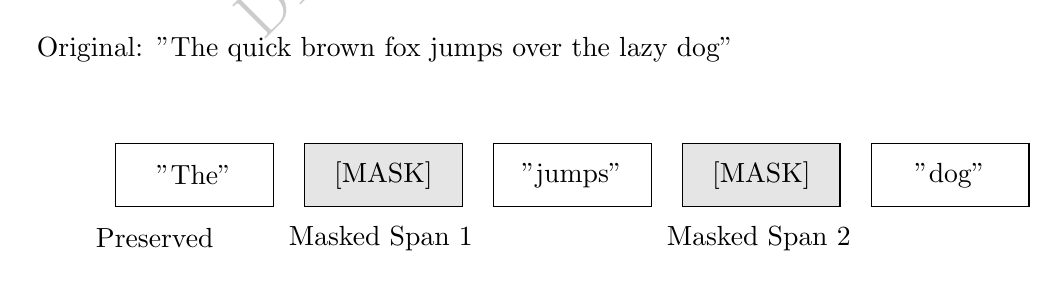
\begin{tikzpicture}[
        scale=0.8,
        box/.style={rectangle, draw, minimum width=2cm, minimum height=0.8cm},
        mask/.style={rectangle, draw, fill=gray!20, minimum width=2cm, minimum height=0.8cm}
    ]
        % Original text
        \node[text width=12cm] at (0,2) {Original: "The quick brown fox jumps over the lazy dog"};
        
        % Masked version
        \node[box] at (-5,0) {"The"};
        \node[mask] at (-2,0) {[MASK]};
        \node[box] at (1,0) {"jumps"};
        \node[mask] at (4,0) {[MASK]};
        \node[box] at (7,0) {"dog"};
        
        % Labels
        \node[text width=2.5cm] at (-5,-1) {Preserved};
        \node[text width=4cm] at (-1,-1) {Masked Span 1};
        \node[text width=4cm] at (5,-1) {Masked Span 2};
    \end{tikzpicture}
    \caption{Span-based masking example where entire phrases are masked together, preserving semantic units.}
    \label{fig:span_masking}
\end{figure} 

\subsection{Prefix Language Modeling}\index{prefix language modeling}
\noindent
This objective combines aspects of causal and masked language modeling to enable both bidirectional context understanding and autoregressive generation:

\begin{itemize}
    \item \textbf{Bidirectional Context}\index{bidirectional context}: Full attention over prefix tokens
    \item \textbf{Autoregressive Generation}\index{autoregressive generation}: Left-to-right generation for suffix
    \item \textbf{Hybrid Attention}\index{hybrid attention}: Different attention patterns for prefix and suffix
\end{itemize}

\begin{figure}[ht]
    \centering
    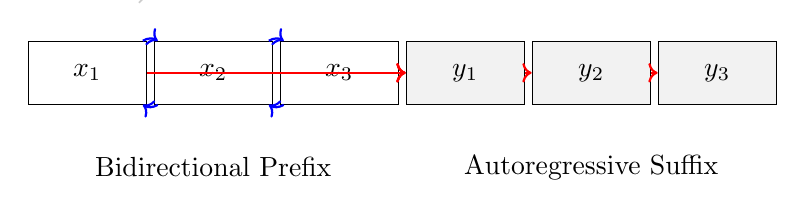
\begin{tikzpicture}[
        scale=0.8,
        token/.style={rectangle, draw, minimum width=1.5cm, minimum height=0.8cm},
        attention/.style={->, thick, blue},
        generation/.style={->, thick, red}
    ]
        % Prefix tokens
        \node[token] (t1) at (0,0) {$x_1$};
        \node[token] (t2) at (2,0) {$x_2$};
        \node[token] (t3) at (4,0) {$x_3$};
        
        % Generation tokens
        \node[token, fill=gray!10] (g1) at (6,0) {$y_1$};
        \node[token, fill=gray!10] (g2) at (8,0) {$y_2$};
        \node[token, fill=gray!10] (g3) at (10,0) {$y_3$};
        
        % Bidirectional attention in prefix
        \draw[attention] (t1) to[bend left=30] (t2);
        \draw[attention] (t2) to[bend left=30] (t3);
        \draw[attention] (t2) to[bend left=30] (t1);
        \draw[attention] (t3) to[bend left=30] (t2);
        
        % Generation attention
        \draw[generation] (t1) -- (g1);
        \draw[generation] (t2) -- (g1);
        \draw[generation] (t3) -- (g1);
        \draw[generation] (g1) -- (g2);
        \draw[generation] (g2) -- (g3);
        
        % Labels
        \node at (2,-1.5) {Bidirectional Prefix};
        \node at (8,-1.5) {Autoregressive Suffix};
    \end{tikzpicture}
    \caption{Prefix language modeling with bidirectional attention in the prefix (blue) and autoregressive attention in the generated suffix (red).}
    \label{fig:prefix_lm}
\end{figure}

\subsection{Contrastive Learning Objectives}\index{contrastive learning}
\noindent
Contrastive learning approaches help models learn better representations by contrasting positive and negative examples:

\begin{itemize}
    \item \textbf{SimCSE}\index{SimCSE}: Uses dropout as minimal augmentation
    \item \textbf{InfoNCE Loss}\index{InfoNCE}: Maximizes mutual information between related contexts
    \item \textbf{Momentum Contrast}\index{momentum contrast}: Maintains dynamic negative samples
\end{itemize}

\begin{equation}
\mathcal{L}_\text{contrast} = -\log \frac{\exp(s(h, h^+)/\tau)}{\sum_{h^- \in \mathcal{N}} \exp(s(h, h^-)/\tau)}
\end{equation}

where $s(\cdot,\cdot)$ is a similarity function and $\tau$ is a temperature parameter.

\section{Multi-Task Pretraining}\index{multi-task pretraining}
\label{sec:multi_task}

\subsection{Auxiliary Objectives}\index{auxiliary objectives}
\noindent
Additional training signals can enhance model learning through complementary tasks that support the main objective. \textbf{Translation Language Modeling (TLM)}\index{translation language modeling} operates by concatenating parallel text segments, enabling the model to learn cross-lingual alignments implicitly and enhance its multilingual capabilities. 

\textbf{Document Rotation Prediction (DRP)}\index{document rotation} challenges the model to predict the original ordering when sentences are randomly rotated, improving discourse understanding. Meanwhile, \textbf{Sentence Boundary Detection (SBD)}\index{sentence boundary detection} focuses on identifying sentence boundaries, helping with document structure comprehension and supporting downstream summarization tasks.

\subsection{Task Mixing Strategies}\index{task mixing}
\noindent
Different approaches to combining multiple objectives during training include \textbf{Fixed Ratio Mixing}\index{fixed ratio mixing}, which uses a weighted sum of task-specific losses:
\begin{equation}
    \mathcal{L}_\text{total} = \sum_{i=1}^{N} \lambda_i \mathcal{L}_i
\end{equation}
where $\lambda_i$ are fixed weights.

\textbf{Dynamic Task Weighting}\index{dynamic task weighting} adjusts the importance of each task based on their relative performance:
\begin{equation}
    \lambda_i(t) = \frac{\exp(-\alpha L_i(t))}{\sum_j \exp(-\alpha L_j(t))}
\end{equation}
where $L_i(t)$ is the loss for task $i$ at step $t$.

\textbf{Uncertainty-Based Weighting}\index{uncertainty-based weighting} determines task weights based on their predictive uncertainty:
\begin{equation}
    \lambda_i = \frac{1}{2\sigma_i^2}
\end{equation}
where $\sigma_i^2$ is the task-specific uncertainty.


\begin{figure}[ht]
    \centering
    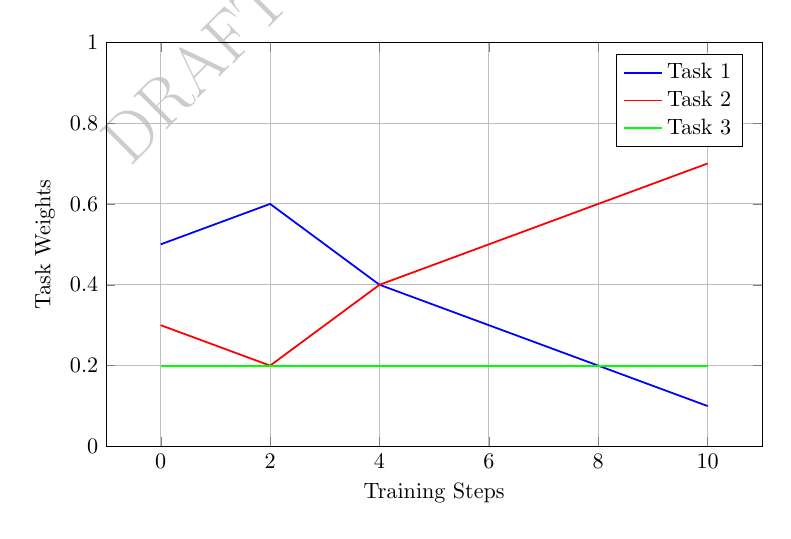
\begin{tikzpicture}[scale=0.8]
        \begin{axis}[
            width=12cm,
            height=8cm,
            xlabel={Training Steps},
            ylabel={Task Weights},
            grid=major,
            legend pos=north east,
            ymin=0, ymax=1
        ]
            % Task weights over time
            \addplot[blue, thick] coordinates {
                (0,0.5) (2,0.6) (4,0.4) (6,0.3) (8,0.2) (10,0.1)
            };
            \addplot[red, thick] coordinates {
                (0,0.3) (2,0.2) (4,0.4) (6,0.5) (8,0.6) (10,0.7)
            };
            \addplot[green, thick] coordinates {
                (0,0.2) (2,0.2) (4,0.2) (6,0.2) (8,0.2) (10,0.2)
            };
            
            \legend{Task 1, Task 2, Task 3}
        \end{axis}
    \end{tikzpicture}
    \caption{Dynamic evolution of task weights during training.}
    \label{fig:task_weights}
\end{figure}

\section{Evaluation Metrics}\index{evaluation metrics}
\label{sec:evaluation}

\subsection{Beyond Perplexity}\index{evaluation!beyond perplexity}
\noindent
While perplexity\index{perplexity} remains important, modern evaluation encompasses broader metrics:

\begin{itemize}
    \item \textbf{Token Prediction Accuracy}\index{token prediction accuracy}
    \begin{equation}
        \text{Accuracy} = \frac{\text{Correct Predictions}}{\text{Total Predictions}}
    \end{equation}
    
    \item \textbf{Bits Per Character (BPC)}\index{bits per character}
    \begin{equation}
        \text{BPC} = -\frac{1}{\log(2)N} \sum_{i=1}^N \log p(x_i)
    \end{equation}
    
    \item \textbf{BLEU Score}\index{BLEU score}
    \begin{equation}
        \text{BLEU} = \text{BP} \cdot \exp\left(\sum_{n=1}^N w_n \log p_n\right)
    \end{equation}
\end{itemize}

\begin{figure}[ht]
    \centering
    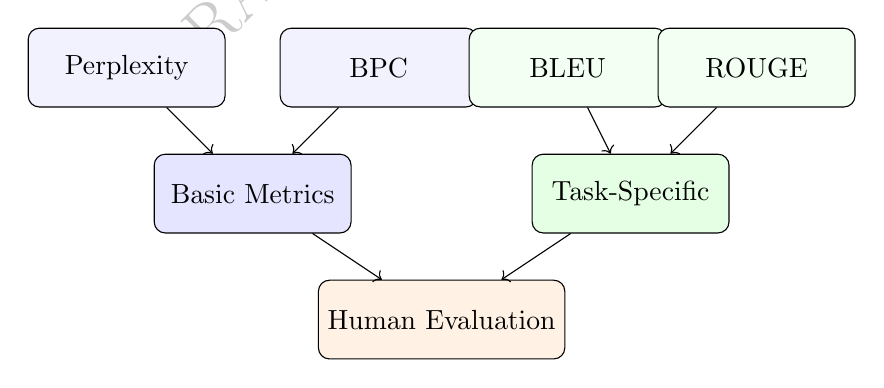
\begin{tikzpicture}[
        scale=0.8,
        metric/.style={rectangle, draw, rounded corners, minimum width=2.5cm, minimum height=1cm}
    ]
        % Metrics categories
        \node[metric, fill=blue!10] (basic) at (0,2) {Basic Metrics};
        \node[metric, fill=green!10] (task) at (6,2) {Task-Specific};
        \node[metric, fill=orange!10] (human) at (3,0) {Human Evaluation};
        
        % Specific metrics
        \node[metric, fill=blue!5] (ppl) at (-2,4) {Perplexity};
        \node[metric, fill=blue!5] (bpc) at (2,4) {BPC};
        \node[metric, fill=green!5] (bleu) at (5,4) {BLEU};
        \node[metric, fill=green!5] (rouge) at (8,4) {ROUGE};
        
        % Connections
        \foreach \i in {ppl,bpc} {
            \draw[->] (\i) -- (basic);
        }
        \foreach \i in {bleu,rouge} {
            \draw[->] (\i) -- (task);
        }
        \draw[->] (basic) -- (human);
        \draw[->] (task) -- (human);
    \end{tikzpicture}
    \caption{Hierarchy of evaluation metrics for language models.}
    \label{fig:evaluation_metrics}
\end{figure}

\subsection{Task-Specific Evaluation}\index{task-specific evaluation}
\noindent
Different downstream tasks require specialized evaluation approaches to accurately measure model performance across various linguistic capabilities:

\subsubsection{Question Answering Metrics}\index{question answering!evaluation}
\noindent
Question answering tasks evaluate both accuracy and comprehension:

\begin{itemize}
    \item \textbf{Exact Match (EM)}\index{exact match}
    \begin{itemize}
        \item Binary score for perfect answer matches
        \item Strict but clear evaluation criterion
        \item Sensitive to minor variations (e.g., punctuation, spacing)
    \end{itemize}
    
    \item \textbf{F1 Score}\index{F1 score}
    \begin{equation}
        \text{F1} = 2 \cdot \frac{\text{precision} \cdot \text{recall}}{\text{precision} + \text{recall}}
    \end{equation}
    \begin{itemize}
        \item Token-level overlap between prediction and ground truth
        \item More forgiving than exact match
        \item Better for partial credit assessment
    \end{itemize}
\end{itemize}

\subsubsection{Text Generation Evaluation}\index{text generation!evaluation}
\noindent
Generation tasks require metrics that can assess both fluency and content:

\begin{itemize}
    \item \textbf{ROUGE Variants}\index{ROUGE}
    \begin{itemize}
        \item ROUGE-N: N-gram overlap
        \item ROUGE-L: Longest common subsequence
        \item ROUGE-S: Skip-bigram co-occurrence
    \end{itemize}
    
    \item \textbf{METEOR}\index{METEOR}
    \begin{itemize}
        \item Incorporates stemming and synonymy
        \item Weighted F-score calculation
        \item Better correlation with human judgments
    \end{itemize}
    
    \item \textbf{CIDEr}\index{CIDEr}
    \begin{itemize}
        \item TF-IDF weighted n-gram similarity
        \item Penalizes common phrases
        \item Domain-adaptive scoring
    \end{itemize}
\end{itemize}

\begin{figure}[ht]
    \centering
    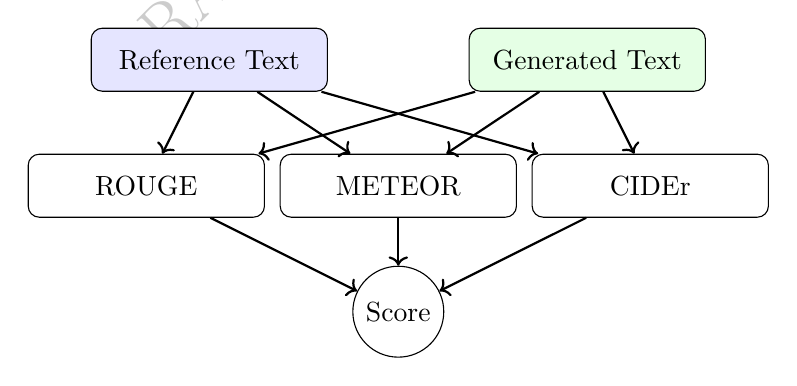
\begin{tikzpicture}[
        scale=0.8,
        box/.style={rectangle, draw, rounded corners, minimum width=3cm, minimum height=0.8cm},
        arrow/.style={->, thick}
    ]
        % Reference and Generated text
        \node[box, fill=blue!10] (ref) at (-3,2) {Reference Text};
        \node[box, fill=green!10] (gen) at (3,2) {Generated Text};
        
        % Metrics
        \node[box] (rouge) at (-4,0) {ROUGE};
        \node[box] (meteor) at (0,0) {METEOR};
        \node[box] (cider) at (4,0) {CIDEr};
        
        % Final score
        \node[circle, draw] (score) at (0,-2) {Score};
        
        % Connections
        \draw[arrow] (ref) -- (rouge);
        \draw[arrow] (ref) -- (meteor);
        \draw[arrow] (ref) -- (cider);
        \draw[arrow] (gen) -- (rouge);
        \draw[arrow] (gen) -- (meteor);
        \draw[arrow] (gen) -- (cider);
        \draw[arrow] (rouge) -- (score);
        \draw[arrow] (meteor) -- (score);
        \draw[arrow] (cider) -- (score);
    \end{tikzpicture}
    \caption{Text generation evaluation pipeline showing multiple metric computation.}
    \label{fig:generation_eval}
\end{figure}

\subsubsection{Semantic Similarity Assessment}\index{semantic similarity!evaluation}
\noindent
Evaluating semantic understanding and representation quality:

\begin{itemize}
    \item \textbf{Embedding-Based Metrics}\index{embedding-based metrics}
    \begin{itemize}
        \item Cosine similarity of sentence embeddings
        \item Word Mover's Distance (WMD)
        \item Contextual embedding comparison
    \end{itemize}
    
    \item \textbf{BERTScore}\index{BERTScore}
    \begin{equation}
        \text{R}_\text{BERT} = \frac{1}{|y|} \sum_{y_i \in y} \max_{x_j \in x} x_j^T y_i
    \end{equation}
    \begin{itemize}
        \item Uses contextual embeddings
        \item Token-level matching
        \item Robust to paraphrasing
    \end{itemize}
    
    \item \textbf{BLEURT}\index{BLEURT}
    \begin{itemize}
        \item Learned metric based on BERT
        \item Fine-tuned on human judgments
        \item Adaptable to specific domains
    \end{itemize}
\end{itemize}

\subsubsection{Human Evaluation Integration}\index{human evaluation}
\noindent
Complementing automatic metrics with human assessment:

\begin{itemize}
    \item \textbf{Likert Scale Ratings}\index{Likert scale}
    \begin{itemize}
        \item Fluency assessment
        \item Factual correctness
        \item Overall quality
    \end{itemize}
    
    \item \textbf{Comparative Evaluation}\index{comparative evaluation}
    \begin{itemize}
        \item A/B testing between models
        \item Relative ranking of outputs
        \item Best-worst scaling
    \end{itemize}
    
    \item \textbf{Error Analysis}\index{error analysis}
    \begin{itemize}
        \item Error categorization
        \item Qualitative feedback
        \item Improvement suggestions
    \end{itemize}
\end{itemize}

\begin{figure}[ht]
    \centering
    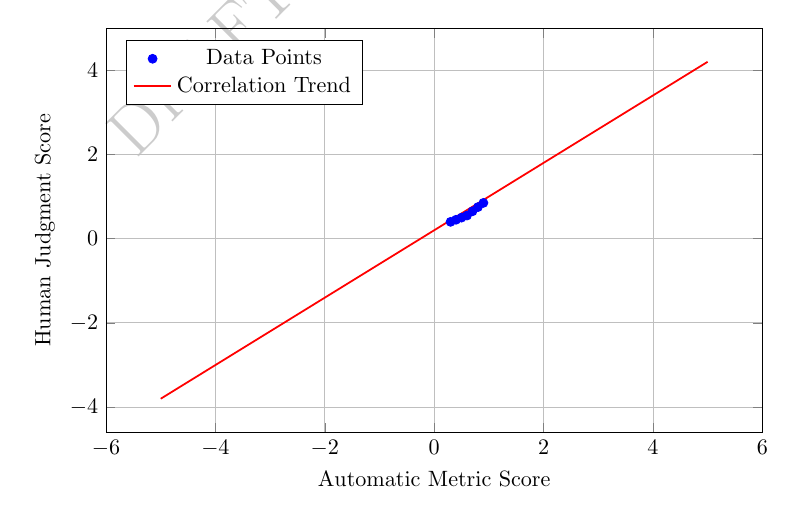
\begin{tikzpicture}[scale=0.8]
        \begin{axis}[
            width=12cm,
            height=8cm,
            xlabel={Automatic Metric Score},
            ylabel={Human Judgment Score},
            grid=major,
            legend pos=north west
        ]
            % Correlation plots
            \addplot[only marks, blue] coordinates {
                (0.3,0.4) (0.4,0.45) (0.5,0.5) (0.6,0.55)
                (0.7,0.65) (0.8,0.75) (0.9,0.85)
            };
            \addplot[red, thick] {0.8*x + 0.2};
            
            \legend{Data Points, Correlation Trend}
        \end{axis}
    \end{tikzpicture}
    \caption{Correlation between automatic metrics and human judgments.}
    \label{fig:human_correlation}
\end{figure}

% Add relevant citations
\nocite{zhang2020bertscore, sellam2020bleurt, papineni2002bleu, banerjee2005meteor}

\chapter{Scaling Laws and Model Behavior}
\label{chap:scaling_laws}

\noindent
As LLMs grow larger, surprising empirical regularities—often termed “scaling laws”—begin to emerge. This chapter explores how model performance, data requirements, and computational costs scale together, and why overparameterized networks can sometimes generalize better than smaller ones. We also discuss practical constraints to keep in mind when deciding how far to scale up.

% PROMPT: Cite recent papers on scaling laws

\noindent
As Large Language Models (LLMs) continue to grow in both parameter count and training data, researchers have empirically observed certain \textbf{scaling laws} governing how model performance scales with size, dataset size, and compute. Studies such as \emph{Kaplan et al. (2020), Hoffmann et al. (2022)} and others have provided insights into how bigger models, when trained on sufficiently large data, can yield significantly improved generalization. Yet, these gains often come at increasing computational and infrastructure costs. This chapter explores the relationships between model scale and performance, the underlying mathematical intuitions behind overparameterization, and the practical constraints that come with building and serving massive models.

\section{Scaling Relationships}
\label{sec:scaling_relationships}
% PROMPT: Empirical laws for model size vs. performance, data size requirements, diminishing returns and capacity

\subsection{Empirical Laws for Model Size vs. Performance}
\noindent
Recent work (\emph{Kaplan et al. (2020)}) suggests that for transformer-based LLMs:
\[
\text{Loss} \sim N_\text{params}^{-\alpha} + N_\text{data}^{-\beta} + \epsilon,
\]
where \(N_\text{params}\) is the number of trainable parameters, \(N_\text{data}\) is the size of the training corpus, and \(\alpha, \beta\) are scaling exponents determined empirically. A key insight is that model performance can be systematically improved by increasing model size \emph{and} data size, up to certain limits.

\subsection{Data Size Requirements}
\noindent
Larger models require correspondingly larger datasets to fully realize their potential. If model capacity far exceeds the amount of training data, overfitting becomes more likely. Conversely, underparameterized models may not effectively utilize massive datasets. Balancing model capacity with dataset size has become a central design consideration:
\begin{itemize}
    \item \textbf{Curated vs. Unfiltered Corpora.} Model performance may plateau if the corpus does not contain sufficiently diverse or high-quality text.
    \item \textbf{Language \& Domain Coverage.} Multilingual or domain-specific LLMs often need specialized datasets to see performance gains relevant to their use cases.
\end{itemize}

\subsection{Diminishing Returns and Capacity}
\noindent
Although scaling up typically yields better performance, gains tend to follow a power-law curve that flattens over time. Each new doubling of parameters or data might yield smaller marginal improvements. This phenomenon poses questions about sustainability and the cost-effectiveness of ever-larger models:
\begin{itemize}
    \item \textbf{Performance Plateaus.} Even if loss decreases, the quantitative improvement in many downstream tasks may become negligible.
    \item \textbf{Overfitting Risks.} If data does not grow in tandem with model size, the model may memorize training examples rather than learning generalizable patterns.
\end{itemize}

\noindent
Understanding these scaling relationships helps practitioners decide how best to allocate resources—whether to invest in model size, data expansion, or specialized architecture tweaks that break conventional scaling laws.

\section{Mathematical Intuition for Overparameterization}
\label{sec:overparameterization_intuition}
% PROMPT: Theorize why overparameterization can sometimes improve generalization

\subsection{Why Bigger Might Be Better (Lottery Ticket Hypothesis, Double Descent)}
\noindent
\textbf{Overparameterization} refers to training models with more parameters than the size of the training dataset might seem to demand. Paradoxically, research has shown that heavily overparameterized networks can still generalize well. Several theories attempt to explain this:

\begin{itemize}
    \item \textbf{Lottery Ticket Hypothesis.} Proposes that within a large neural network, there exist smaller \emph{subnetworks} (“winning tickets”) that, if trained in isolation from the beginning, could achieve performance comparable to the full network. Overparameterization increases the probability of containing such winning subnetworks.

    \item \textbf{Double Descent.} Introduces a phenomenon where increasing model capacity first reduces error, then enters a regime of poor performance (when the model is just large enough to overfit), and finally improves again as the model grows even larger. The second descent happens as the model transitions from the interpolation regime to a more complex, smoother representation, yielding better generalization.
\end{itemize}

\subsection{Inductive Biases Learned by LLMs}
\noindent
Large Transformer-based models can learn \textbf{inductive biases} favoring functions that generalize, even in extremely high-dimensional parameter spaces:
\begin{itemize}
    \item \textbf{Sparse and Low-Rank Patterns.} Attention mechanisms and factorized embeddings can capture sparse or low-rank structures in language, aiding generalization.
    \item \textbf{Compositionality and Hierarchical Representations.} Depth and multi-head attention encourage the layering of linguistic features, from surface form to semantic abstractions, making large models surprisingly robust.
\end{itemize}

\noindent
While these explanations remain an active research area, they underscore a key takeaway: overparameterized LLMs are not simply memorizing data. Under certain conditions—especially with ample training data and regularization—they can discover more powerful and generalized representations than smaller counterparts.

\section{Practical Constraints}
\label{sec:practical_constraints}
% PROMPT: Mention typical hardware setups for large-scale training

\subsection{Hardware Limitations (GPU/TPU Memory, Compute Time)}
\noindent
\textbf{Scaling LLMs} requires substantial computational infrastructure:
\begin{itemize}
    \item \textbf{GPU/TPU Memory.} Large batch sizes and parameter counts quickly exceed single-device memory. Techniques like tensor/model parallelism, pipeline parallelism, and sharded optimizers become mandatory for feasible training.
    \item \textbf{Compute Hours.} Training a multi-billion parameter model can take days or weeks on hundreds of GPUs/TPUs. This cost can be prohibitive for many research labs and organizations.
    \item \textbf{Networking Bottlenecks.} Distributed training necessitates high-bandwidth interconnects (e.g., NVLink, Infiniband) to synchronize gradients efficiently.
\end{itemize}

\subsection{Budgeting for Training}
\noindent
Aside from technical challenges, the financial and environmental costs of training large models are non-trivial:
\begin{itemize}
    \item \textbf{Cloud Compute vs. On-Prem Clusters.} Organizations must weigh the elasticity and speed of cloud services against the capital costs and control benefits of building on-premises HPC systems.
    \item \textbf{Energy Consumption.} Training billion-parameter models can have a sizable carbon footprint. Efforts to optimize training efficiency, including algorithmic improvements and better hardware utilization, are increasingly important.
    \item \textbf{Maintenance \& Model Retraining.} Once trained, models often require periodic retraining with updated data or domain-specific fine-tuning, further adding to long-term operational costs.
\end{itemize}

\noindent
In essence, while scaling up model size and data can yield impressive performance gains, it also raises engineering, financial, and ethical questions about cost-effectiveness and sustainability. Researchers and practitioners must balance the promise of larger models against these practical constraints, seeking new methods to achieve \emph{efficient} scaling without compromising on capabilities.

\chapter{Data Preparation for Large Language Models}
\label{chap:data_preparation}

\noindent
Building a Large Language Model (LLM)\index{LLM|see {Large Language Model}}\index{Large Language Model} begins with assembling and preprocessing\index{preprocessing} massive text corpora that reflect the linguistic richness and domain diversity needed to train a high-capacity model. Careful data curation\index{data!curation}, cleaning\index{data!cleaning}, and tokenization\index{tokenization} significantly influence a model's final performance and behavior. In this chapter, we explore the key steps in preparing data for LLM training, drawing on practices from large-scale projects such as \emph{GPT-3} (Brown et al., 2020) and \emph{BERT} (Devlin et al., 2019), as well as community efforts like \emph{The Pile} (Gao et al., 2021). Our discussion covers data sourcing, filtering, deduplication, normalization, and the final conversion of text into tokenized sequences.

\section{Data Sources and Collection}\index{data!sources}
\noindent
LLMs typically require hundreds of gigabytes to terabytes of text. This sheer volume necessitates collecting data from a variety of sources:
\begin{itemize}
    \item \textbf{Web Crawls}\index{web crawls}\index{Common Crawl} (Common Crawl)
    \item \textbf{Curated Corpora}\index{curated corpora}
    \item \textbf{Proprietary or Domain-Specific Data}\index{domain-specific data}
\end{itemize}

\noindent
\textbf{Importance of Data Diversity.} 
Having texts from multiple genres (news, conversations, scientific papers, novels, social media) helps the model learn different registers, writing styles, and vocabularies. Overreliance on a single source can bias the model toward that style and limit its coverage.

\section{Filtering and Cleaning}\index{data!filtering}\index{data!cleaning}
\noindent
Raw web data often contains noise such as boilerplate text, malformed markup, or offensive content. \textbf{Filtering and cleaning} steps help ensure a usable dataset:
\begin{itemize}
    \item \textbf{Language Detection.} Models may be primarily trained in English or target multiple languages. Automated language identification tools (e.g., \texttt{langid.py}) filter out texts misclassified or containing very little in the desired language(s).
    \item \textbf{Boilerplate Removal.} Web crawls can contain duplicates of navigation bars, ads, or repeated disclaimers. Deduplication scripts or boilerplate detectors (e.g., \texttt{jusText}, \texttt{trafilatura}) strip out non-content text.
    \item \textbf{Offensive/NSFW Filtering.} Projects like GPT-3 used keyword lists, blocklists, and classifier-based approaches to remove extreme hate speech, sexual content, or personally identifiable information. The exact filtering threshold can vary, balancing open-domain coverage with ethical/legal constraints.
    \item \textbf{Data Quality Checks.} Very short documents, empty lines, or texts with excessive repetition can be removed. Some pipelines also filter by perplexity scores from smaller "quality-check" language models, discarding outlier documents likely to be nonsensical.
\end{itemize}

\noindent
\textbf{Case Example: GPT-3.}  
In their dataset, OpenAI curated 499 billion tokens. They performed multiple levels of filtering—first removing duplicates, non-English content, and extremely short or low-quality documents, then using domain- and style-based heuristics to refine the final corpus (Brown et al., 2020).

\section{Deduplication}\index{deduplication} and Dataset Overlap
\noindent
LLMs can inadvertently learn to \emph{memorize} large chunks of text—particularly if the same passages appear multiple times in the training set. Deduplication is thus essential to:
\begin{itemize}
    \item \textbf{Avoid Overfitting.} Repeated sequences artificially reduce the model's training loss on these passages and limit generalization.
    \item \textbf{Minimize Copyright Risks.} Duplication of copyrighted text increases the chance of regurgitating it verbatim during inference.
\end{itemize}

\noindent
\textbf{Approaches to Deduplication.}
\begin{itemize}
    \item \emph{Exact String Matching.} Simple but fast approach that finds exact duplicates of entire documents or large n-grams.
    \item \emph{Approximate/MinHashing.} Employs locality-sensitive hashing to identify near-duplicates. Widely used in large-scale corpora to handle minor edits or formatting differences.
    \item \emph{Segment-Level Fingerprinting.} Breaks texts into overlapping segments, generating fingerprints for each. This identifies partial duplicates across large corpora more robustly.
\end{itemize}
Comprehensive deduplication ensures a more \emph{varied} dataset and reduces the chance of unintentional memorization.

\section{Text Normalization}\index{text normalization} and Preprocessing
\noindent
Once filtered, text often undergoes normalization steps to remove extraneous characters and maintain consistent formatting:
\begin{itemize}
    \item \textbf{Unicode Normalization.} Converts characters to a standard form (e.g., NFC) to handle accented letters or compatibility forms.
    \item \textbf{Lowercasing (Optional).} While many modern tokenizers handle case, some pipelines choose to lowercase text (especially for smaller vocabularies). However, lowercasing discards capitalization cues, which can be relevant for named entities or acronyms.
    \item \textbf{Whitespace Cleanup.} Strips unnecessary line breaks, tabs, or multiple spaces.
    \item \textbf{URL, Email Removal or Replacement.} In some cases, URLs or emails are replaced with special tokens (\texttt{<URL>}, \texttt{<EMAIL>}) to preserve context without retaining sensitive info.
\end{itemize}

\noindent
\textbf{Choosing a Consistent Preprocessing Scheme.}  
Consistency across the entire dataset is crucial. If half the data is lowercased and the other half is not, the model's vocabulary distribution becomes more complex, leading to potential confusion during training.

\section{Tokenization}\index{tokenization}
\noindent
\textbf{Tokenization} converts text into a sequence of discrete tokens that the model can process. Modern LLMs often employ \textbf{subword}\index{subword tokenization} tokenization methods:
\begin{itemize}
    \item \textbf{Byte-Pair Encoding}\index{BPE|see {Byte-Pair Encoding}}\index{Byte-Pair Encoding} (BPE)
    \item \textbf{WordPiece}\index{WordPiece}
    \item \textbf{SentencePiece}\index{SentencePiece}
\end{itemize}

\noindent
\textbf{Vocabulary Size Trade-offs.}
\begin{itemize}
    \item A \emph{larger vocabulary} reduces sequence lengths (since words are less frequently split), but can lead to more model parameters (due to embedding tables) and potential data sparsity issues for rare subwords.
    \item A \emph{smaller vocabulary} makes the model handle more subword splits, potentially capturing morphological variations better, but with longer token sequences and higher computational costs per sample.
\end{itemize}

\section{Data Sharding}\index{data!sharding} and Batching\index{batching}
\noindent
Training an LLM typically involves distributing data across multiple GPUs or TPUs:
\begin{itemize}
    \item \textbf{Sharding.} The dataset is often split into "shards"—each shard is a chunk of the dataset stored separately. Large-scale frameworks (e.g., \texttt{Apache Arrow}, \texttt{WebDataset}) streamline sharding and distributed loading.
    \item \textbf{Curriculum vs. Random Sampling.} While random sampling is the default, some pipelines explore \emph{curriculum learning}, starting with simpler or more relevant text first. However, curriculum schedules can add complexity.
    \item \textbf{Mini-Batch Construction.} Batches must be efficiently formed from shards to maintain high throughput. Large batch sizes accelerate training but require appropriate learning rate adjustments.
\end{itemize}

\noindent
\textbf{Case Example: BERT Pretraining on TPU Pods.}  
BERT's original training used 16 Cloud TPUs, each processing distinct shards in parallel, with synchronized gradient updates (\emph{Devlin et al. 2019}). This approach required careful pre-shuffling and sharding to maintain data diversity across accelerator replicas.

\section{Validation Sets}\index{validation sets} and Data Splits\index{data!splits}
\noindent
To track overfitting and model progress, it is crucial to maintain well-defined validation sets:
\begin{itemize}
    \item \textbf{Held-Out Validation.} Randomly sampled from the entire dataset. In large-scale training, this may be a fraction of a percent but still yields millions of tokens for reliable evaluation.
    \item \textbf{Domain-Specific Splits.} Some practitioners create domain-specific or specialized test sets (e.g., legal or biomedical) to evaluate domain transfer or out-of-distribution robustness.
    \item \textbf{Public Benchmarks.} Standard tasks (GLUE, SuperGLUE, SQuAD, etc.) are not strictly part of the pretraining corpus but serve as final evaluation to check real-world applicability.
\end{itemize}

\noindent
\textbf{Note on "Contamination."}  
To avoid data leakage (where test examples appear in the training corpus), it is best practice to cross-check validation/test sets against the training data. Efforts like \emph{The Pile} apply rigorous checks to identify overlaps with popular benchmarks.

\section{Ethical and Legal Considerations}\index{ethics}\index{legal considerations}
\noindent
As LLMs become more powerful, data preparation intersects with ethical and legal constraints:
\begin{itemize}
    \item \textbf{Privacy.} Personal data or sensitive user-generated content must be removed or anonymized to comply with regulations like GDPR. 
    \item \textbf{Bias Mitigation.} Over-representation of certain demographics or topics can embed social biases. Strategies to counteract bias might involve balancing domains or applying fairness filters.
    \item \textbf{Copyright.} Large crawls can contain copyrighted material. Dataset creators must decide how to handle or filter copyrighted text to reduce legal risk.
\end{itemize}

\noindent
\textbf{Transparency and Documentation.}  
Initiatives like \emph{Datasheets for Datasets} (Gebru et al.) call for clear documentation of data origins, preprocessing steps, and potential limitations. Such transparency fosters responsible LLM deployment.

\section{Summary and Best Practices}
\noindent
Data preparation can be the \textbf{largest engineering effort} in training an LLM. Key takeaways and practices include:
\begin{itemize}
    \item \textbf{Diverse Sourcing.} Aim for coverage across multiple domains, languages, and writing styles to build robust general-purpose models.
    \item \textbf{Thorough Cleaning \& Filtering.} Removing noise and offensive or duplicative content improves both performance and ethical safety.
    \item \textbf{Careful Tokenization.} Select a suitable subword method and vocabulary size, noting trade-offs between sequence length and representational granularity.
    \item \textbf{Deduplication.} Prevent memorization and reduce the risk of regurgitating copyrighted or sensitive text.
    \item \textbf{Ethical Review.} Ensure privacy, fairness, and compliance measures are in place, reflecting the societal impact of LLMs.
\end{itemize}

\bigskip
\noindent
Overall, \textbf{data preparation} lays the foundation upon which Large Language Models are built. While training and model architecture often receive the spotlight, the success—or pitfalls—of an LLM often stem from the quality and diversity of its underlying corpus. By applying robust filtering, scaling up responsibly, and documenting every step, practitioners can create high-caliber datasets that drive state-of-the-art results in NLP. 


\part{Advanced Topics and Future Directions}
\chapter{Fine-Tuning and Prompt Engineering}\index{fine-tuning}\index{prompt engineering}
\label{chap:fine_tuning_prompt}

\noindent
Modern Large Language Models (LLMs)\index{LLM|see {Large Language Model}} are typically trained on massive corpora in a self-supervised manner\index{self-supervised training}, after which they can be adapted to specific tasks or domains via \textbf{fine-tuning}\index{fine-tuning!definition} or \textbf{prompt engineering}\index{prompt engineering!definition}. This chapter explores different approaches to fine-tuning—both full\index{fine-tuning!full} and parameter-efficient\index{fine-tuning!parameter-efficient}—and demonstrates how strategically designed prompts can elicit strong zero-shot\index{zero-shot} and few-shot\index{few-shot} performance from LLMs.

\section{The Fine-Tuning Spectrum}\index{fine-tuning!spectrum}
\noindent
Fine-tuning represents a continuum of adaptation approaches, ranging from full model updates to minimal parameter modifications:

\subsection{Full Fine-Tuning}\index{fine-tuning!full}
\noindent
Traditional fine-tuning updates all model parameters on task-specific data. While this approach offers maximum flexibility, it presents several challenges:

\textbf{Resource Requirements.}\index{fine-tuning!resource requirements} Full fine-tuning of large models demands substantial computational resources, often requiring distributed training across multiple GPUs. For example, fine-tuning a 175B parameter model might require hundreds or thousands of GPU hours.

\textbf{Catastrophic Forgetting.}\index{catastrophic forgetting} Aggressive fine-tuning can cause the model to "forget" its pre-trained knowledge, especially with small datasets. This necessitates careful learning rate scheduling and early stopping strategies.

\textbf{Storage Overhead.}\index{storage overhead} Each fine-tuned version requires storing a complete copy of the model parameters, making it impractical to maintain multiple task-specific variants of large models.

\subsection{Parameter-Efficient Fine-Tuning}\index{fine-tuning!parameter-efficient}
\noindent
Recent advances have introduced methods that update only a small subset of parameters or add a small number of new parameters:

\textbf{LoRA (Low-Rank Adaptation)}\index{LoRA} decomposes weight updates into low-rank matrices, dramatically reducing the number of trainable parameters while maintaining performance. The mathematical foundations and implementation details are covered in Section~\ref{subsec:lora}.

\textbf{Prompt Tuning}\index{prompt tuning} learns continuous prompt embeddings while keeping the base model frozen. This approach offers several advantages:
\begin{itemize}
    \item Minimal parameter overhead (typically <1% of model size)
    \item Easy task switching by swapping prompt embeddings
    \item Competitive performance with full fine-tuning on many tasks
\end{itemize}

\section{Prompt Engineering Strategies}\index{prompt engineering!strategies}
\noindent
Effective prompt engineering requires understanding both the capabilities and limitations of LLMs. Key strategies include:

\subsection{Chain-of-Thought Prompting}\index{chain-of-thought prompting}
\noindent
This technique encourages step-by-step reasoning by demonstrating intermediate thought processes in the prompt. For example:

\begin{verbatim}
Q: A shirt costs $25. If there's a 20% discount, what's the final price?
A: Let's solve this step by step:
1. Calculate 20% of $25: $25 × 0.20 = $5
2. Subtract the discount: $25 - $5 = $20
Therefore, the final price is $20.
\end{verbatim}

\subsection{Role and Context Specification}\index{prompt engineering!role specification}
\noindent
Clearly defining the model's role and context can significantly improve output quality:

\begin{verbatim}
You are an expert mathematician explaining concepts to a high school student.
Explain the quadratic formula in simple terms, using real-world examples.
\end{verbatim}

\section{Hybrid Approaches}\index{hybrid approaches}
\noindent
Many modern applications combine fine-tuning and prompt engineering:

\textbf{Instruction Tuning + Prompting}\index{instruction tuning} involves fine-tuning on instruction-following data, then using carefully crafted prompts to guide the model's behavior. This approach has proven particularly effective for complex reasoning tasks.

\textbf{Few-Shot Learning with Fine-Tuned Models}\index{few-shot learning} uses fine-tuning to improve the model's base capabilities, then leverages few-shot prompting for task-specific adaptation. This combination often achieves better results than either approach alone.

\section{Evaluation and Iteration}\index{evaluation}
\noindent
Developing effective fine-tuning and prompting strategies requires systematic evaluation and iteration:

\textbf{Quantitative Metrics}\index{evaluation!metrics} include task-specific measures like accuracy, F1-score, and ROUGE, as well as general metrics like perplexity and cross-entropy.

\textbf{Qualitative Analysis}\index{evaluation!qualitative} involves manual review of model outputs, focusing on:
\begin{itemize}
    \item Consistency across similar inputs
    \item Adherence to specified constraints
    \item Quality of reasoning and explanations
    \item Handling of edge cases
\end{itemize}

% PROMPT: Show a side-by-side comparison of full fine-tuning vs. LoRA
\section{Methods of Fine-Tuning}\index{fine-tuning!methods}
\label{sec:methods_finetune}

\noindent
Fine-tuning typically involves updating a model's parameters on a target dataset\index{dataset!target} after it has been pre-trained\index{pre-training} on a large, diverse corpus. However, \emph{full fine-tuning}\index{fine-tuning!full} can be computationally expensive\index{computational cost} and may risk overfitting\index{overfitting} on smaller datasets. Recent research has introduced \textbf{parameter-efficient}\index{parameter efficiency} approaches that significantly reduce the number of trainable parameters while preserving performance.

\subsubsection*{Full Fine-Tuning vs. LoRA (High-Level Comparison)}
\begin{center}
\renewcommand{\arraystretch}{1.3}
\begin{tabular}{p{0.25\textwidth} | p{0.3\textwidth} p{0.3\textwidth}}
\hline
\textbf{Aspect} & \textbf{Full Fine-Tuning} & \textbf{LoRA} \\ \hline
\textbf{Trainable Parameters} 
& \(\sim\!100\%\) of the model's parameters are updated 
& Only a small fraction of parameters (low-rank matrices) are updated \\

\textbf{Memory Footprint} 
& High: must store and backprop through all parameters 
& Low: minimal overhead; the base model can be frozen \\

\textbf{Speed of Training} 
& Slower, as gradients must be computed for all layers 
& Faster, due to fewer trainable parameters \\

\textbf{Risk of Overfitting} 
& Potentially higher, especially with small datasets 
& Lower, since fewer parameters adapt \& the rest remain fixed \\

\textbf{Common Use Cases} 
& When you have a large dataset and enough compute to adapt the entire model 
& When compute/memory are limited or the target dataset is relatively small \\ \hline
\end{tabular}
\end{center}

\subsection{Low-Rank Adaptation (LoRA)}\index{LoRA}\index{low-rank adaptation}
\label{subsec:lora}
% Mathematical formulation of LoRA
\begin{itemize}
    \item Traditional weight updates vs. LoRA's low-rank decomposition
    \item Matrix factorization approach: 
    \begin{equation}\label{eq:lora_decomp}
    W + BA \text{ where } B \in \mathbb{R}^{d \times r}, A \in \mathbb{R}^{r \times k}
    \end{equation}
    \item Rank $r$ as a hyperparameter controlling capacity vs. efficiency trade-off
\end{itemize}

% Implementation details
\begin{pythoncode}[LoRA Implementation]
import torch
import torch.nn as nn
import math

class LoRALayer:
    def __init__(self, base_layer, rank=4, alpha=1.0):
        self.base_layer = base_layer
        self.rank = rank
        self.alpha = alpha
        
        # Initialize A and B matrices
        self.lora_A = nn.Parameter(torch.zeros(rank, base_layer.weight.size(1)))
        self.lora_B = nn.Parameter(torch.zeros(base_layer.weight.size(0), rank))
        nn.init.kaiming_uniform_(self.lora_A, a=math.sqrt(5))
        nn.init.zeros_(self.lora_B)
        
    def forward(self, x):
        # Regular forward pass
        base_output = self.base_layer(x)
        
        # LoRA adjustment
        lora_output = (self.lora_B @ self.lora_A @ x.T).T * (self.alpha / self.rank)
        
        return base_output + lora_output
\end{pythoncode}

% Advantages and practical considerations
\begin{itemize}
    \item Memory efficiency: Only training 
    \begin{equation}\label{eq:lora_params}
    r(d + k) \text{ parameters instead of } dk
    \end{equation}
    \item Faster training and inference compared to full fine-tuning
    \item Ability to merge LoRA weights with base model for deployment
\end{itemize}

% Mathematical analysis
\begin{itemize}
    \item Theoretical foundations of low-rank updates
    \item Impact on model capacity and expressiveness
    \item Relationship to other parameter-efficient methods
\end{itemize}

% Empirical results and best practices
\begin{itemize}
    \item Typical rank values for different tasks
    \item Guidelines for setting the scaling factor $\alpha$
    \item Performance comparisons with full fine-tuning
\end{itemize} 

\subsection{Other Parameter-Efficient Methods}\index{parameter-efficient methods}
\noindent
Beyond LoRA, several other techniques aim to reduce the computational and memory costs\index{memory costs} of fine-tuning:
\begin{itemize}
    \item \textbf{Adapters.}\index{adapters} Introduced in the context of computer vision\index{computer vision} and NLP\index{NLP}, \emph{adapters} insert small "bottleneck" layers\index{bottleneck layers} in each block of a Transformer. Only these adapter layers are trained, while the rest of the parameters remain frozen.
    \item \textbf{Prompt Tuning / Prefix Tuning.}\index{prompt tuning}\index{prefix tuning} Instead of modifying the model's core parameters, special "prompt" or "prefix" tokens\index{tokens!prompt}\index{tokens!prefix} are learned and prepended to the input sequence. The base model weights remain static, relying on these learned vectors to steer predictions.
    \item \textbf{BitFit.}\index{BitFit} Proposes fine-tuning only the bias terms\index{bias terms} in each layer, drastically reducing the parameter footprint while retaining moderate performance.
\end{itemize}

\noindent
All these methods share a common goal: retain most of the pre-trained model's knowledge while introducing minimal, task-specific parameter updates. This can be crucial when dealing with large models where full fine-tuning becomes prohibitively expensive.

% PROMPT: Demonstrate a few-shot prompting scenario
\section{Prompt Engineering and In-Context Learning}\index{prompt engineering}\index{in-context learning}
\label{sec:prompt_engineering}

\noindent
\textbf{Prompt engineering}\index{prompt engineering!techniques} manipulates the input context\index{input context} presented to an LLM to guide its output behavior, often without updating any model parameters at all. This approach relies on the idea of \emph{in-context learning}\index{in-context learning!definition}: the model's attention mechanism\index{attention mechanism} can glean instructions and few-shot examples\index{few-shot examples} directly from the prompt.

\subsection{Few-Shot and Zero-Shot Prompting}\index{prompting!few-shot}\index{prompting!zero-shot}
\begin{itemize}
    \item \textbf{Zero-Shot Prompting.}\index{zero-shot!prompting} The model is given only a task description\index{task description} or question without explicit in-task examples. For instance:
\begin{verbatim}
"Explain in simple terms why the sky is blue."
\end{verbatim}
    \item \textbf{Few-Shot Prompting.}\index{few-shot!prompting} A small number of demonstrations\index{demonstrations} (input-output examples\index{examples!input-output}) are included in the prompt. For example:
\begin{verbatim}
 Q: What is the capital of France? 
 A: Paris

 Q: What is the capital of Germany?
 A: Berlin
\end{verbatim}
  The model observes the pattern (question -> answer) and often completes the final answer correctly.
\end{itemize}

\noindent
\textbf{Why It Works:} The multi-head self-attention in Transformers effectively reweights relevant parts of the prompt. This "hint" or "instruction" setup can drastically improve performance on tasks for which the model hasn't been explicitly fine-tuned.

\subsection{The Math Behind Attention Re-Weighting}\index{attention!re-weighting}
\noindent
When you prepend or inject prompt tokens into the sequence, they become part of the \(\mathbf{Q}, \mathbf{K}, \mathbf{V}\) matrices\index{attention!matrices} in the \textbf{scaled dot-product attention}\index{attention!scaled dot-product}:
\[
\text{Attention}(\mathbf{Q}, \mathbf{K}, \mathbf{V}) = \text{softmax}\Bigl(\frac{\mathbf{Q}\mathbf{K}^\top}{\sqrt{d_k}}\Bigr)\,\mathbf{V}.
\]
The inserted prompt tokens can influence:
\begin{itemize}
    \item Which tokens the model "attends" to in a few-shot example (keys/values).
    \item How strongly the model weights certain prompt tokens (queries).
\end{itemize}
In effect, the \emph{prompt} guides the attention distribution to emulate training examples on the fly.

% PROMPT: Recommend metrics for zero-shot vs. fine-tuned models
\section{Evaluation Metrics and Challenges}\index{evaluation!metrics}\index{evaluation!challenges}
\label{sec:metrics_challenges}

\subsection{BLEU, ROUGE, Perplexity, and Beyond}\index{BLEU}\index{ROUGE}\index{perplexity}
\noindent
When assessing the quality of outputs—whether from zero-shot prompts or fine-tuned models—common \textbf{automatic metrics}\index{metrics!automatic} include:
\begin{itemize}
    \item \textbf{BLEU}\index{BLEU!definition} Measures n-gram overlap\index{n-gram overlap} between generated text and reference translations; popular in machine translation.
    \item \textbf{ROUGE}\index{ROUGE!definition} Focuses on recall of n-grams or sequences for summarization tasks\index{summarization}.
    \item \textbf{Perplexity}\index{perplexity!definition} Often used to gauge how well the language model predicts a sequence. Lower perplexity means the model is less "surprised" by the data.
    \item \textbf{Other Task-Specific Metrics.} Accuracy, F1-score, or exact match for classification and QA tasks; meteor, CIDEr, or SPICE for image-caption tasks.
\end{itemize}

\subsection{Human vs. Automated Evaluations}\index{evaluation!human}\index{evaluation!automated}
\noindent
\textbf{Automatic metrics}\index{metrics!automatic} are convenient but may not capture nuanced qualities such as factual correctness\index{factual correctness}, coherence\index{coherence}, and style\index{style}. For tasks like open-ended generation\index{generation!open-ended} or complex QA\index{question answering}, \textbf{human evaluations}\index{evaluation!human} often remain the gold standard:
\begin{itemize}
    \item \textbf{Annotator Bias.} Human reviewers might be inconsistent or exhibit bias in judging model outputs, necessitating structured guidelines or multiple reviewers.
    \item \textbf{Cost and Scalability.} Large-scale human evaluations are expensive and time-consuming, so hybrid approaches that combine automatic filtering with targeted human checks are common.
\end{itemize}

\noindent
In practice, balancing \emph{automated metrics} with periodic \emph{human assessments} tends to yield the best insights into an LLM's true capabilities and limitations—especially in scenarios where precision and reliability are paramount.

\bigskip
\noindent
\textbf{Summary.} Fine-tuning and prompt engineering represent two complementary paths to adapt powerful pre-trained LLMs to specific tasks and contexts. While full fine-tuning modifies all of a model's parameters, LoRA and other parameter-efficient techniques drastically reduce resource demands. Meanwhile, effective prompting can elicit strong few-shot and zero-shot performance without altering a single weight. By coupling these adaptation methods with appropriate evaluation strategies, practitioners can leverage the full breadth of modern LLMs' capabilities. 

\section{Fine-Tuning and Prompt Engineering}
\label{sec:fine_tuning}

\noindent
As models grow larger~\cite{brown2020language}, efficient fine-tuning becomes crucial. Methods like LoRA~\cite{hu2021lora} and QLoRA~\cite{dettmers2023qlora} enable parameter-efficient adaptation...

Instruction tuning~\cite{ouyang2022training} has emerged as a powerful way to improve model capabilities.

\chapter{Large Language Model Mixture-of-Experts}\index{Mixture-of-Experts}\index{LLM!Mixture-of-Experts}\index{MoE|see{Mixture-of-Experts}}
\label{chap:moe}

\section{Introduction}
\noindent
Mixture-of-Experts (MoE)\index{Mixture-of-Experts!introduction} is a neural network architecture\index{neural network!architecture} that has recently gained significant attention, particularly in the field of large language models (LLMs)\index{LLM!architecture}. MoE models offer a way to dramatically increase model capacity\index{model capacity} without a proportional increase in computational cost\index{computational cost} during inference\index{inference}. This is achieved by conditionally activating\index{conditional activation} only a subset of the network for each input token. This chapter explores the architecture, implementation, and implications of MoE in modern LLMs.

\section{What is Mixture-of-Experts?}
\label{sec:moe_basics}

\subsection{Core Concepts}
\noindent
The core idea behind MoE\index{Mixture-of-Experts!core concepts} is to divide a complex task into smaller, more manageable subtasks\index{subtasks}. Each subtask is handled by a specialized "expert" network\index{expert network}, and a "gating network"\index{gating network} decides which expert(s) should be activated for a given input.

\subsection{Components of an MoE Model}
\noindent
An MoE layer typically consists of the following key components:
\begin{itemize}
    \item \textbf{Expert Networks:} Feed-forward networks specialized in processing specific aspects of the data
    \item \textbf{Gating Network:} Determines expert allocation using learned routing functions
    \item \textbf{Router:} Implements the actual routing mechanism (e.g., top-k routing)
    \item \textbf{Combiner:} Aggregates expert outputs into the final layer output
\end{itemize}

\begin{figure}[ht]
\centering
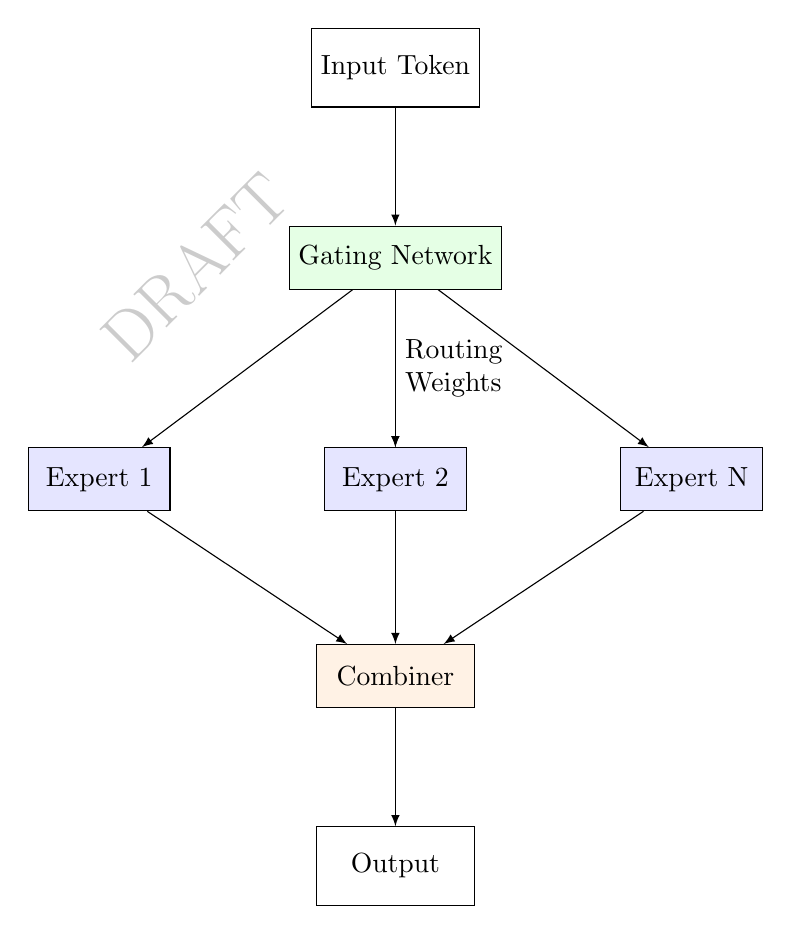
\begin{tikzpicture}[
    node distance=1.5cm,
    box/.style={rectangle, draw, minimum width=2cm, minimum height=1cm},
    expert/.style={rectangle, draw, fill=blue!10, minimum width=1.8cm, minimum height=0.8cm},
    gate/.style={rectangle, draw, fill=green!10, minimum width=2.5cm, minimum height=0.8cm},
    combine/.style={rectangle, draw, fill=orange!10, minimum width=2cm, minimum height=0.8cm}
]
    % Input
    \node[box] (input) {Input Token};
    
    % Gating Network
    \node[gate] (gate) [below=of input] {Gating Network};
    
    % Experts
    \node[expert] (exp1) [below left=2cm and 1.5cm of gate] {Expert 1};
    \node[expert] (exp2) [below=2cm of gate] {Expert 2};
    \node[expert] (exp3) [below right=2cm and 1.5cm of gate] {Expert N};
    %\node[text width=1cm] (dots) [below=2cm of gate, xshift=0.8cm] {...};
    
    % Combiner
    \node[combine] (combine) [below=4.5cm of gate] {Combiner};
    
    % Output
    \node[box] (output) [below=of combine] {Output};
    
    % Arrows
    \draw[-latex] (input) -- (gate);
    \draw[-latex] (gate) -- (exp1);
    \draw[-latex] (gate) -- (exp2);
    \draw[-latex] (gate) -- (exp3);
    \draw[-latex] (exp1) -- (combine);
    \draw[-latex] (exp2) -- (combine);
    \draw[-latex] (exp3) -- (combine);
    \draw[-latex] (combine) -- (output);
    
    % Router weights
    \draw[-latex, dashed] (gate) -- node[right, text width=2cm] {Routing Weights} (exp2);
\end{tikzpicture}
\caption{Architecture of a Mixture-of-Experts (MoE) layer. The gating network determines which experts process the input token, and the combiner aggregates their outputs weighted by the routing weights.}
\label{fig:moe_architecture}
\end{figure}

\subsection{Mathematical Formulation}
\noindent
For input $x$ with $N$ experts $E_1, \ldots, E_N$ and gating network $G$, the output $Y$ is:
\[
Y(x) = \sum_{i=1}^{N} G(x)_i \cdot E_i(x)
\]
where $G(x)_i$ represents the gating weight for expert $i$.

\section{MoE Architectures in LLMs}
\label{sec:moe_architectures}

\subsection{Sparse MoE}
\noindent
Modern LLMs typically use sparse MoE where only a small subset of experts process each token:
\begin{itemize}
    \item \textbf{Top-k Routing:} Only the k highest-scoring experts are activated
    \item \textbf{Token-level Routing:} Different tokens can be routed to different experts
    \item \textbf{Expert Capacity:} Managing maximum tokens per expert during training
\end{itemize}

\subsection{Switch Transformers}
\noindent
Switch Transformers~\cite{fedus2021switch} introduce simplified routing where each token is assigned to exactly one expert, reducing routing complexity while maintaining performance.

\subsection{Mixture of Experts in Modern LLMs}
\noindent
Recent implementations in production models:
\begin{itemize}
    \item \textbf{GShard:} Google's distributed MoE implementation
    \item \textbf{GLaM:} Efficiently scaled trillion-parameter models
    \item \textbf{Mixtral 8x7B:} Open-source sparse MoE model
\end{itemize}

\section{Training MoE Models}
\label{sec:moe_training}

\subsection{Load Balancing}
\noindent
Critical training considerations include:
\begin{itemize}
    \item \textbf{Auxiliary Loss:} Encouraging uniform expert utilization
    \item \textbf{Capacity Factor:} Managing expert overflow during training
    \item \textbf{Dynamic Expert Selection:} Adapting routing patterns during training
\end{itemize}

\subsection{Distributed Training}
\noindent
Strategies for efficient distributed training:
\begin{itemize}
    \item \textbf{Expert Parallelism:} Distributing experts across devices
    \item \textbf{All-to-All Communication:} Managing expert routing overhead
    \item \textbf{Load Balancing:} Ensuring efficient device utilization
\end{itemize}

\section{Benefits and Challenges}
\label{sec:moe_benefits_challenges}

\subsection{Advantages}
\begin{itemize}
    \item \textbf{Conditional Computation:} Activating only relevant parameters
    \item \textbf{Scalability:} Increasing capacity without proportional compute
    \item \textbf{Specialization:} Experts focusing on specific language aspects
    \item \textbf{Parameter Efficiency:} Better performance per active parameter
\end{itemize}

\subsection{Challenges}
\begin{itemize}
    \item \textbf{Training Instability:} Complex optimization dynamics
    \item \textbf{Communication Overhead:} All-to-all communication costs
    \item \textbf{Load Balancing:} Ensuring uniform expert utilization
    \item \textbf{Implementation Complexity:} Complex routing and distributed training
\end{itemize}

\section{Future Directions}
\label{sec:moe_future}

\subsection{Research Frontiers}
\begin{itemize}
    \item \textbf{Dynamic Architecture:} Adaptive expert addition/removal
    \item \textbf{Hierarchical Routing:} Multi-level expert selection
    \item \textbf{Hardware-Aware Design:} Optimizing for specific accelerators
    \item \textbf{Sparse-to-Dense Distillation:} Knowledge transfer to smaller models
\end{itemize}

\subsection{Emerging Applications}
\begin{itemize}
    \item \textbf{Multi-Modal MoE:} Extending to vision and audio
    \item \textbf{Task-Specific Experts:} Specialization for different domains
    \item \textbf{Efficient Deployment:} Edge and mobile optimization
\end{itemize}

\section{Conclusion}
\noindent
MoE architectures represent a significant advancement in scaling LLMs efficiently. By enabling sparse activation and increased model capacity, they offer a promising direction for future model development. While challenges remain in training stability, load balancing, and implementation complexity, ongoing research continues to address these issues, making MoE an increasingly attractive approach for next-generation language models.

% Add relevant citations
\nocite{shazeer2017outrageously, lepikhin2020gshard, fedus2021switch, du2021glam, mistral2023mixtral}
\chapter{Emergent Abilities and Interpretability}\index{emergent abilities}\index{interpretability}
\label{chap:emergent_interpretability}
% PROMPT: Give examples of complex reasoning tasks LLMs can handle

\noindent
As Large Language Models (LLMs)\index{LLM|see {Large Language Model}} increase in parameter count\index{parameters!count} and training data\index{training data}, they often exhibit \textbf{emergent abilities}\index{emergent abilities!definition}—capabilities that were not explicitly programmed or observed in smaller-scale variants. These abilities can range from improved contextual understanding\index{contextual understanding} to complex multi-step reasoning\index{reasoning!multi-step}. Simultaneously, the \textbf{interpretability}\index{interpretability!definition} of these models becomes a pressing concern, driving the development of techniques to reveal how and why LLMs make certain decisions. This chapter examines such emergent behaviors\index{emergent behaviors}, discusses common interpretability tools\index{interpretability!tools}, and addresses pressing topics in safety\index{safety}, bias\index{bias}, and ethics\index{ethics}.

\section{Emergent Behaviors}\index{emergent behaviors}
\label{sec:emergent_behaviors}
% PROMPT: Give examples of complex reasoning tasks LLMs can handle

\subsection{"Chain-of-Thought" Reasoning and Large Model Capabilities}\index{chain-of-thought}\index{reasoning capabilities}
\noindent
One widely discussed emergent property is the tendency of larger LLMs to showcase \textbf{chain-of-thought} (CoT)\index{chain-of-thought!reasoning} reasoning. Rather than providing a single-step answer, the model can generate intermediate reasoning steps\index{reasoning!steps}:
\begin{itemize}
    \item \textbf{Multi-Step Arithmetic.}\index{arithmetic!multi-step} Large models can solve math problems\index{math problems} by outlining intermediate steps, mimicking human-like problem-solving workflows\index{problem-solving}.
    \item \textbf{Logical Reasoning.}\index{reasoning!logical} With sufficient parameters and training, LLMs can handle if-then reasoning\index{if-then reasoning}, analogies\index{analogies}, and rudimentary symbolic manipulations\index{symbolic manipulation}.
    \item \textbf{Contextual Coherence.}\index{coherence!contextual} In discourse-level tasks\index{discourse tasks}, bigger models more consistently maintain context across multiple sentences or paragraphs, reducing contradictions\index{contradictions}.
\end{itemize}
Interestingly, enabling chain-of-thought explicitly in prompts (e.g., “Let’s think this through step by step...”) can further enhance performance on reasoning-heavy tasks, despite no explicit \emph{supervision} for such multi-step outputs during pretraining.

\subsection{Breakdown of Tasks That LLMs Excel At vs. Struggle With}
\noindent
While LLMs can exhibit surprising competence in areas like translation, summarization, and Q\&A, they continue to face challenges:
\begin{itemize}
    \item \textbf{Excel:} 
    \begin{itemize}
        \item \emph{Natural Language Understanding:} Recognizing context, paraphrasing, and semantic nuances.
        \item \emph{Creative Text Generation:} Producing coherent stories, headlines, or poetry.
        \item \emph{Few-Shot Generalization:} Leveraging large pretraining corpora to adapt quickly to new tasks through examples in the prompt.
    \end{itemize}
    \item \textbf{Struggle:}
    \begin{itemize}
        \item \emph{Complex Symbolic or Numerical Reasoning:} Multi-hop inference with strict logic can still be error-prone without specialized prompts or fine-tuning.
        \item \emph{Factual Reliability:} LLMs sometimes produce hallucinations or spurious facts, requiring robust verification.
        \item \emph{Commonsense Knowledge Gaps:} Though less frequent at scale, certain real-world knowledge or reasoning about physical processes can be inconsistent.
    \end{itemize}
\end{itemize}


\section{Interpretability Tools}\index{interpretability!tools}
\label{sec:interpretability_tools}
% PROMPT: Provide a sample attention visualization

\subsection{Attention Visualization, Gradient-Based Explanations}\index{attention!visualization}\index{gradient-based explanations}
\noindent
\textbf{Attention mechanisms}\index{attention!mechanisms} in Transformers are often viewed as a natural gateway to interpretability. By visualizing attention weights\index{attention!weights}, one can see which tokens the model "focuses on" for a particular prediction:
\begin{itemize}
    \item \textbf{Heatmap of Attention Scores.}\index{attention!scores}\index{heatmap} Plotting attention weights between each query token and all key tokens can provide insights into how context is integrated. For instance, a heatmap revealing that the model consistently attends to a subject noun when predicting a verb could signal a grammatical or semantic alignment.
    \item \textbf{Gradient-Based Methods.}\index{gradient methods} Techniques like \emph{Grad-CAM}\index{Grad-CAM} highlight how changes in input tokens affect the model's output. By computing gradients of the output w.r.t. input embeddings, one can locate crucial tokens driving predictions.
\end{itemize}

\noindent
Below is a simplified snippet of how one might visualize attention weights in Python (pseudocode):

\begin{verbatim}
import matplotlib.pyplot as plt

def visualize_attention(attention_weights, tokens, head=0, layer=0):
    attn = attention_weights[layer][head].detach().cpu().numpy()
    fig, ax = plt.subplots()
    cax = ax.matshow(attn, cmap='viridis')
    fig.colorbar(cax)
    ax.set_xticklabels(['']+tokens, rotation=90)
    ax.set_yticklabels(['']+tokens)
    plt.show()
\end{verbatim}

\subsection{Attribution Methods (Integrated Gradients, etc.)}
\noindent
\textbf{Attribution methods} attempt to quantify each input token's importance for the model's final decision. Examples include:
\begin{itemize}
    \item \textbf{Integrated Gradients (IG).} Measures the integral of the gradients of the model's output w.r.t. the inputs along a path from a baseline (e.g., zero embeddings) to the actual input. IG can help address the saturation problem of simpler gradient-based explanations.
    \item \textbf{Layer-wise Relevance Propagation (LRP).} Propagates the model's output backward through the network, distributing "relevance" scores across input features.
\end{itemize}

\noindent
These methods provide complementary viewpoints to attention visualizations, especially since attention scores do not necessarily equate to a direct measure of causal attribution. Employing multiple interpretability tools offers a more holistic understanding of how LLMs generate their outputs.


\section{Safety, Bias, and Ethics}\index{safety}\index{bias}\index{ethics}
\label{sec:safety_bias_ethics}
% PROMPT: Discuss how to measure and mitigate bias in LLMs

\noindent
The powerful generative capabilities of LLMs can amplify existing societal biases, produce harmful or offensive content, and misinform users. These risks underscore the need for ongoing research and systematic evaluations of \textbf{model safety}, \textbf{bias}, and \textbf{fairness}.

\subsection{Mathematical Perspectives on Bias Measurement}\index{bias!measurement}
\noindent
\textbf{Bias} in LLMs can be framed as disparities in model outputs across demographic groups\index{demographic groups} or protected categories\index{protected categories}. Formalizing such biases often involves:
\begin{itemize}
    \item \textbf{Distribution Shifts.}\index{distribution shifts} Comparing performance or output distributions across different subsets of data (e.g., texts referencing different genders or ethnicities).
    \item \textbf{Statistical Parity.}\index{statistical parity} Ensuring the model's predictions do not disproportionately favor or harm specific groups. In classification settings, one might measure the difference in positive prediction rates between groups.
    \item \textbf{Calibration Curves.}\index{calibration curves} Assessing how well the model's predicted probabilities align with true outcome frequencies for different groups or input conditions.
\end{itemize}
While these metrics can be adapted to generative contexts (e.g., analyzing word usage or sentiment across demographic references), the open-ended nature of LLM outputs complicates the analysis.

\subsection{Calibration, Uncertainty, and Fairness Metrics}\index{calibration}\index{uncertainty}\index{fairness metrics}
\noindent
Related to bias, \textbf{calibration}\index{calibration!definition} pertains to the model's confidence estimates—i.e., whether a token probability reflects the actual likelihood of correctness. Poor calibration can mask or exacerbate biased predictions. \textbf{Fairness metrics}\index{fairness!metrics}, such as \emph{Equalized Odds}\index{Equalized Odds} or \emph{Equal Opportunity}\index{Equal Opportunity}, aim to align the model's behavior across subpopulations\index{subpopulations} without sacrificing overall performance\index{performance}. For LLMs:
\begin{itemize}
    \item \textbf{Prompt-Based Adjustments.} Carefully crafted instructions or disclaimers can steer the model away from producing biased or offensive content.
    \item \textbf{Filtering \& Post-Processing.} Deployed LLM systems often incorporate content filters or re-ranking modules to remove inappropriate generations.
    \item \textbf{Fine-Tuning on Diverse Data.} Domain- or demographic-specific datasets can help mitigate biases, though care must be taken to balance representation.
\end{itemize}

\noindent
Ensuring safety, fairness, and ethical use of LLMs is not a one-time step but an iterative process requiring interdisciplinary collaboration among ML practitioners, domain experts, and ethicists. As models grow in size and capability, so too must the rigor of interpretability and bias mitigation strategies.

\bigskip
\noindent
\textbf{Summary.} Emergent behaviors in LLMs—such as chain-of-thought reasoning—highlight the rapidly evolving landscape of AI capabilities. However, along with these new strengths come increased demands for \emph{interpretability} and \emph{safeguards} against biased or harmful outputs. By harnessing attention visualization, attribution methods, and robust bias measurement tools, researchers and developers can better understand these models' internal workings, ultimately guiding LLMs toward more trustworthy and equitable deployments.

\section{Emergent Abilities}
\label{sec:emergent_abilities}

\noindent
Recent research~\cite{wei2022emergent} has documented surprising capabilities that emerge abruptly when models reach certain parameter thresholds. These abilities are not present in smaller models and appear discontinuously rather than through gradual improvement. Examples include:
\begin{itemize}
    \item \textbf{Multi-step reasoning} emerging around 100B parameters
    \item \textbf{Code generation} becoming reliable at 20-50B parameters
    \item \textbf{Zero-shot task following} appearing beyond 50B parameters
\end{itemize}

\noindent
Open-source models like LLaMA~\cite{touvron2023llama}, LLaMA 2~\cite{touvron2023llama2}, and research models like PaLM~\cite{chowdhery2022palm} and GPT-4~\cite{openai2023gpt4} have demonstrated these emergent properties at scale. Notably, these capabilities often appear suddenly across multiple benchmarks simultaneously, suggesting fundamental shifts in model comprehension rather than task-specific improvements.

\chapter{Efficient Serving and Deployment}
\label{chap:serving_deployment}

\noindent
Deploying Large Language Models (LLMs) in real-world applications entails challenges related to \textbf{latency}, \textbf{memory}, and \textbf{scalability}. Although training can be distributed over vast compute clusters, end-user queries demand rapid inference, often with limited hardware resources. This chapter explores \textbf{model compression} techniques like distillation and quantization, discusses strategies for low-latency inference, and outlines architectural approaches for serving large-scale LLMs.

% PROMPT: Compare quantization methods (e.g., 8-bit, 4-bit)
\section{Model Distillation and Compression}
\label{sec:distillation_compression}

\subsection{Teacher-Student Framework}
\noindent
\textbf{Knowledge distillation} compresses a large “teacher” model into a smaller “student” model by transferring the teacher’s output distribution. Formally, if \(\mathbf{z}_\text{teacher}\) is the teacher’s logits for a given input, and \(\mathbf{z}_\text{student}\) is the student’s logits, we minimize:
\[
\mathcal{L}_\text{KD} = \text{KL}\Bigl(\sigma\bigl(\frac{\mathbf{z}_\text{teacher}}{T}\bigr),\, \sigma\bigl(\frac{\mathbf{z}_\text{student}}{T}\bigr)\Bigr),
\]
where \(\sigma(\cdot)\) is typically the softmax function and \(T\) is a temperature parameter that smooths distributions. Key advantages include:
\begin{itemize}
    \item \textbf{Reduced Model Size.} Smaller models demand fewer parameters and thus less memory at inference.
    \item \textbf{Retained Performance.} If the student matches teacher outputs well, performance can remain strong on the downstream task.
    \item \textbf{Faster Inference.} Fewer parameters and a smaller compute graph enable lower-latency predictions.
\end{itemize}

\subsection{Quantization, Pruning, and the Math Behind It}
\noindent
Beyond distillation, \textbf{quantization} and \textbf{pruning} are key strategies to reduce the compute and memory footprint:

\begin{itemize}
    \item \textbf{Quantization.}
    \begin{itemize}
        \item \textbf{8-bit (INT8) Quantization.} We replace 32-bit or 16-bit floating-point weights with 8-bit integers. This significantly lowers memory and speeds up matrix multiplication on specialized hardware. However, some models can suffer an accuracy drop unless quantization-aware training or calibration is applied.
        \item \textbf{4-bit or Lower.} Further compression is possible with 4-bit quantization, but the risk of information loss grows. Methods like \emph{Adaptive Rounding} and \emph{ZeroQuant} attempt to mitigate accuracy degradation by learning optimal quantization boundaries.
    \end{itemize}

    \item \textbf{Pruning.}
    \begin{itemize}
        \item \textbf{Unstructured Pruning.} Sets a percentage of weights to zero (based on magnitude or other criteria) and stores a sparse matrix representation. This can reduce memory, but speed-ups require specialized sparse-matrix operations.
        \item \textbf{Structured Pruning.} Removes entire filters or attention heads, yielding a smaller, dense model architecture that more naturally translates to inference speed-ups on standard hardware.
    \end{itemize}
\end{itemize}

\noindent
By combining pruning with quantization (and even distillation), one can achieve considerable compression factors, often with minimal performance loss—especially when the original model has large redundancy.

% PROMPT: Illustrate how to handle batching during inference
\section{Latency Considerations}
\label{sec:latency_considerations}

\subsection{Transformer Inference Optimizations (Kernel Fusion, GPU Acceleration)}
\noindent
\textbf{Inference latency} can be broken down into:
\begin{itemize}
    \item \textbf{Computation Time.} Matrix multiplications for attention and feedforward sub-layers dominate runtime. \emph{Kernel fusion} merges multiple small operations into a single GPU kernel, reducing overhead. 
    \item \textbf{Memory Transfer.} Minimizing data movement between CPU and GPU is crucial. Techniques like \emph{pinning memory} and \emph{asynchronous transfers} can help.
    \item \textbf{Caching Key/Value.} For auto-regressive generation, caching past key/value vectors obviates re-computation of entire attention layers at each step, drastically speeding up decoding.
\end{itemize}

\subsection{Batch vs. Streaming Inference}
\noindent
Balancing throughput and latency is often a matter of \textbf{batching} strategy:
\begin{itemize}
    \item \textbf{Batch Inference.} Multiple queries are batched together to exploit GPU parallelism. This yields high throughput but can introduce higher latency for individual requests.
    \item \textbf{Streaming (Real-Time) Inference.} Queries are processed as soon as they arrive, providing lower latency but lower overall throughput. This is common in interactive applications like chatbots or real-time translation.
\end{itemize}

\noindent
Systems may dynamically switch between modes or maintain separate services to handle high-throughput vs. low-latency user demands. For example, an application might offer a real-time conversation agent as well as a separate batch processing service for large-scale text generation tasks.

% PROMPT: Propose different deployment strategies for large-scale LLMs
\section{Serving Architectures}
\label{sec:serving_architectures}

\subsection{Distributed Serving Strategies}
\noindent
When dealing with \textbf{large-scale LLMs}, single-node inference can be insufficient:
\begin{itemize}
    \item \textbf{Model Parallelism.} The model is split across multiple GPUs in a single server or across servers, each holding a subset of the parameters. During inference, tensors are exchanged via high-speed interconnects (e.g., NVLink, InfiniBand).
    \item \textbf{Pipeline Parallelism.} Different layers (or sets of layers) are placed on different devices. Input data flows through the pipeline from layer group to layer group. This approach is effective for very large models but requires careful scheduling to avoid idle devices.
    \item \textbf{Sharding \& Parameter Server.} A parameter server architecture can store large model parameters in a distributed fashion, with each compute node querying the parameter server for required weights at inference time. 
\end{itemize}

\subsection{Memory Sharing and Caching for LLMs}
\noindent
Even after compression, LLMs can remain too large for single-device deployment. \textbf{Memory sharing} strategies can help:
\begin{itemize}
    \item \textbf{Shared CPU/GPU Offloading.} Weights not immediately needed for a token computation can be offloaded to CPU memory, then reloaded when required.
    \item \textbf{In-Memory Caching of Key-Value Pairs.} For auto-regressive tasks, storing key/value matrices for each user session can enable rapid generation of the next token without recomputing earlier attention states.
    \item \textbf{Multi-Instance Deployment.} Splitting traffic across multiple instances of the same model can help manage memory footprints while scaling horizontally. A load balancer routes user requests to an available instance, each with a local cache of partial computations.
\end{itemize}

\noindent
Choosing the right serving architecture depends on a variety of factors, including \emph{user traffic patterns}, \emph{latency requirements}, and \emph{infrastructure constraints}. By combining compression techniques, GPU optimizations, and parallel serving strategies, organizations can deploy powerful LLMs that meet demanding performance targets without incurring runaway operational costs.

\bigskip
\noindent
\textbf{Summary.} Deploying large-scale LLMs in production environments is often as challenging as training them. \emph{Distillation}, \emph{quantization}, and \emph{pruning} help reduce model size and inference time. \emph{Batching}, \emph{streaming}, and \emph{caching} strategies further optimize throughput and latency. Finally, \emph{distributed serving architectures} ensure the model remains responsive even under heavy workloads. Collectively, these approaches form a toolkit for making LLMs both \textbf{efficient} and \textbf{scalable} in real-world applications.

\chapter{Benchmarking Large Language Models}\index{benchmarking}\index{language models!benchmarking}
\label{chap:benchmarking_llms}

\noindent
As Large Language Models (LLMs) evolve in capacity and sophistication, rigorous \textbf{benchmarking}\index{benchmarking!rigor} becomes ever more important to assess their true capabilities. Benchmarks serve as standardized measures of performance across tasks ranging from basic text classification to complex reasoning. In this chapter, we explore the landscape of existing benchmarks for LLMs, discuss the evaluation metrics they employ, and consider the emerging challenges in designing fair and representative tests for these models.

\section{Why Benchmark LLMs?}\index{benchmarking!importance}
\noindent
Benchmarks offer a consistent yardstick for comparing different models, hyperparameter configurations, or architectural choices. They enable:
\begin{itemize}
    \item \textbf{Progress Tracking.}\index{progress tracking} Researchers can observe trends in model performance over time, attributing improvements (or regressions) to specific design choices or increased model scale.
    \item \textbf{Reproducibility.}\index{reproducibility} Public benchmark datasets and standardized scoring protocols help ensure that reported results are comparable across different research groups and institutions.
    \item \textbf{Task Diversity.}\index{task diversity} Modern NLP requires handling a wide array of tasks (e.g., summarization, translation, QA). Benchmarks aggregate these tasks, giving a holistic view of a model’s language understanding and generation skills.
    \item \textbf{Model Limitations.}\index{model limitations} Through error analysis on benchmark tasks, researchers identify the specific weaknesses of a model—for instance, struggles with long-context reasoning, numerical calculations, or factual correctness.
\end{itemize}

\noindent
However, benchmarks are imperfect proxies for real-world performance. They often focus on \emph{static} or \emph{single-domain} tasks, which may not capture all the nuances of open-ended user interactions.

\section{Popular Benchmarks and Their Scope}\index{benchmarks}
\noindent
The NLP community has produced numerous benchmark suites tailored to different objectives. Below, we highlight some of the most influential ones.

\subsection{GLUE and SuperGLUE}\index{GLUE}\index{SuperGLUE}
\noindent
\textbf{General Language Understanding Evaluation (GLUE)}\index{GLUE!definition}\index{language understanding!evaluation} \cite{wang2018glue} is a multi-task benchmark containing nine diverse tasks (e.g., text classification, semantic similarity, natural language inference). It focuses on \emph{general language understanding}. SuperGLUE \cite{wang2019superglue} is a harder successor, incorporating tasks that are more challenging, like Winograd Schema adversarial examples.

\begin{itemize}
    \item \textbf{Strengths:} 
        \begin{itemize}
            \item Covers a variety of sentence- or paragraph-level NLP tasks. 
            \item Provides a leaderboard that has spurred rapid progress.
        \end{itemize}
    \item \textbf{Limitations:}
        \begin{itemize}
            \item Relatively small datasets—top LLMs can saturate near-human scores.
            \item Emphasizes classification and inference, with fewer generative tasks.
        \end{itemize}
\end{itemize}

\subsection{SQuAD and Open-Domain QA Benchmarks}\index{SQuAD}\index{Open-Domain QA}
\noindent
Reading comprehension benchmarks like \textbf{SQuAD (Stanford Question Answering Dataset)} \cite{rajpurkar2016squad} evaluate the ability of a model to extract or generate answers to factual questions from a given passage.

\begin{itemize}
    \item \textbf{SQuAD 2.0} includes unanswerable questions, testing a model’s ability to abstain if insufficient information is present.
    \item \textbf{Open-Domain QA} benchmarks (e.g., Natural Questions, TriviaQA) challenge models to find answers across large text corpora (like Wikipedia), emphasizing retrieval and factual correctness.
\end{itemize}

\noindent
Modern LLMs often excel at SQuAD-style tasks, but may still falter on less-structured real-world queries or tasks requiring multiple hops of reasoning.

\subsection{BIG-Bench (BBH) and Other Broad Evaluations}\index{BIG-Bench}
\noindent
\textbf{BIG-Bench} (and its subset, \textbf{BIG-Bench Hard}, or BBH) \cite{srivastava2022beyond} is a collaborative project that collects a wide range of \emph{creative} and \emph{unusual} tasks from the community. It goes beyond standard classification or QA:
\begin{itemize}
    \item \textbf{Covers Complex Reasoning.} Includes tasks like logical puzzles, code reasoning, or multi-step math.
    \item \textbf{Open-Ended Generation.} Some tasks require essay-style answers, exploring coherence and creativity.
\end{itemize}

\noindent
Because of its breadth, BIG-Bench acts as a stress test, revealing emergent weaknesses or unusual failure modes in large models. Other broad evaluations, like \textbf{HELLO-SimpleAI} and \textbf{HumanEval} (for code generation), are also emerging to test specific capabilities.

\subsection{MT, Summarization, and Specialized Benchmarks}\index{Machine Translation}\index{Text Summarization}
\noindent
\textbf{Machine Translation (MT).}\index{machine translation!benchmarks}\index{WMT}\index{translation metrics} Benchmarks such as WMT (\emph{Workshop on Machine Translation}) annually test models on bilingual translation across multiple language pairs. Metrics like \textit{BLEU} and \textit{CHRF} measure the closeness of generated translations to reference texts.

\textbf{Text Summarization.}\index{summarization!benchmarks}\index{ROUGE}\index{CNN/DailyMail dataset} Datasets like CNN/DailyMail, XSum, and Gigaword evaluate abstractive summarization quality. Common metrics include \textit{ROUGE} to measure overlap with human summaries.

\textbf{Domain-Specific Benchmarks.} Various specialized benchmarks exist for domains such as biomedical text (\textbf{BioNLP}), legal text (\textbf{LEDGAR}), and code generation (\textbf{HumanEval}, \textbf{CodeXGLUE}). These tasks ensure that models are robust when faced with domain jargon and specific knowledge demands.

\section{Evaluation Metrics and Methodologies}\index{evaluation metrics}
\noindent
\textbf{Automatic metrics}\index{metrics!automatic}\index{evaluation!automatic} like accuracy\index{accuracy}, F1 score\index{F1 score}, BLEU\index{BLEU}, ROUGE\index{ROUGE}, or perplexity\index{perplexity} provide quick quantitative estimates of performance. However, modern LLMs—especially those capable of free-form generation—demand more nuanced assessments:
\begin{itemize}
    \item \textbf{Human Evaluation.}\index{human evaluation} For tasks like creative writing, summarization, or dialogue, human judgments remain the gold standard. Annotators rate outputs for correctness, coherence, style, or helpfulness.
    \item \textbf{Composite Scores.}\index{composite scores} Some benchmarks report aggregated scores across tasks (e.g., GLUE’s average). This single metric can hide per-task nuances but simplifies model-to-model comparisons.
    \item \textbf{Task-Specific Metrics.}\index{task-specific metrics} Complex tasks may require custom evaluation protocols (e.g., logical puzzle correctness, multi-step chain-of-thought coherence, code execution correctness).
\end{itemize}

\noindent
Additionally, \textbf{few-shot}\index{few-shot evaluation} and \textbf{zero-shot}\index{zero-shot evaluation} evaluations have gained popularity, where models must handle tasks without fine-tuning or with minimal example prompts. This tests the generalization abilities learned in pretraining.

\section{Challenges in Benchmarking Large Language Models}\index{challenges}
\noindent
Despite the value of benchmarking, several challenges arise when evaluating LLMs at scale:
\begin{itemize}
    \item \textbf{Data Contamination.}\index{data contamination} With massive training corpora, LLMs may have seen parts of benchmark test sets during pretraining. This inflates scores and reduces the validity of the benchmark as a measure of true generalization.
    \item \textbf{Benchmark Saturation.}\index{benchmark saturation} Many benchmarks have seen near-human or even superhuman performance from top LLMs, making them less discriminative for future advances.
    \item \textbf{One-Dimensional Metrics.}\index{one-dimensional metrics} Single-number metrics often fail to capture qualitative aspects like creativity, fairness, or reliability under adversarial inputs.
    \item \textbf{Evolving Tasks.}\index{evolving tasks} Real-world tasks evolve (e.g., updated knowledge, new social norms). Static benchmarks may lag behind current user needs.
\end{itemize}

\noindent
Addressing these issues requires \emph{continual benchmark revision}, improved data curation, and more holistic or adaptive evaluation frameworks.

\section{Emerging Directions in Evaluation}\index{emerging directions}
\noindent
As LLMs move toward more general-purpose, interactive AI systems, the community has begun experimenting with:
\begin{itemize}
    \item \textbf{Interactive Benchmarks.}\index{interactive benchmarks} Platforms where models are dynamically tested via multi-turn dialogue or real-time tasks (e.g., an environment for code debugging).
    \item \textbf{Adversarial Testing.}\index{adversarial testing} Crowdsourced or automated frameworks generate tricky inputs (ambiguous questions, rhetorical forms, or illusions) to push models beyond standard dataset distributions.
    \item \textbf{Ethical and Bias Metrics.}\index{ethical metrics}\index{bias metrics} Researchers are introducing bias detection benchmarks (e.g., measuring offensive language, gender bias) and testing for safe completion of sensitive queries.
    \item \textbf{Explainability Tasks.}\index{explainability} Evaluations that require chain-of-thought or step-by-step justifications to measure how well the model can \emph{explain} its predictions.
\end{itemize}

\noindent
These newer benchmarks try to better reflect real human interactions, social contexts, and the need for robust and interpretable outputs.

\section{Practical Tips for Benchmarking}\index{practical tips}
\noindent
To get the most out of benchmarking experiments:
\begin{itemize}
    \item \textbf{Check Data Leakage.}\index{data leakage} If possible, cross-reference your training corpus with benchmark test sets and remove any overlaps.
    \item \textbf{Report Multiple Metrics.}\index{multiple metrics} Combine automatic metrics with human evaluation or error analysis to capture multiple facets of performance.
    \item \textbf{Document Hyperparameters and Prompts.}\index{hyperparameters} LLM responses can be sensitive to prompt phrasing, temperature settings, or chain-of-thought instructions. Transparency ensures reproducibility.
    \item \textbf{Track Variance.}\index{variance} Large models can exhibit run-to-run variability. Reporting average scores over multiple seeds or runs can give a more reliable estimate.
    \item \textbf{Use Representative Checkpoints.}\index{checkpoints} For large-scale experiments, you may checkpoint models periodically rather than only at the final epoch. This can help reveal learning trajectories.
\end{itemize}


\section{Existing Benchmarks for Evaluating LLMs}

 This section provides an overview of common LLM benchmarks, categorized by the specific aspect of language understanding they are designed to assess.

\subsection{General Language Understanding and Reasoning}

This category encompasses benchmarks that test a model's overall ability to understand and reason with natural language across a variety of tasks.

\begin{itemize}
    \item \textbf{GLUE (General Language Understanding Evaluation)} \cite{wang2018glue}: A seminal benchmark comprising nine diverse NLU tasks.
    \begin{itemize}
        \item \textbf{CoLA (Corpus of Linguistic Acceptability)}: Assessing grammatical correctness.
        \item \textbf{SST-2 (Stanford Sentiment Treebank)}: Binary sentiment classification.
        \item \textbf{MRPC (Microsoft Research Paraphrase Corpus)}: Paraphrase detection.
        \item \textbf{STS-B (Semantic Textual Similarity Benchmark)}: Measuring semantic similarity on a continuous scale.
        \item \textbf{QQP (Quora Question Pairs)}: Detecting semantically equivalent questions.
        \item \textbf{MNLI (Multi-Genre Natural Language Inference)}: Textual entailment across diverse genres.
        \item \textbf{QNLI (Question Natural Language Inference)}: Question-answering based entailment.
        \item \textbf{RTE (Recognizing Textual Entailment)}: Binary textual entailment classification.
        \item \textbf{WNLI (Winograd Natural Language Inference)}: Coreference resolution based entailment.
    \end{itemize}
    \item \textbf{SuperGLUE} \cite{wang2019superglue}: A more challenging successor to GLUE, featuring harder tasks and more robust evaluation methods.
    \begin{itemize}
        \item \textbf{BoolQ} \cite{clark2019boolq}: Yes/no question answering.
        \item \textbf{CB (CommitmentBank)} \cite{de2019commitmentbank}: Identifying the author's commitment level towards a statement.
        \item \textbf{COPA (Choice of Plausible Alternatives)} \cite{roemmele2011choice}: Selecting the most plausible cause or effect.
        \item \textbf{MultiRC (Multi-Sentence Reading Comprehension)} \cite{khashabi2018looking}: Answering questions requiring multi-sentence reasoning.
        \item \textbf{ReCoRD (Reading Comprehension with Commonsense Reasoning Dataset)} \cite{zhang2018record}: Cloze-style reading comprehension requiring commonsense reasoning.
        \item \textbf{RTE (Recognizing Textual Entailment)}: Same as in GLUE.
        \item \textbf{WiC (Word-in-Context)} \cite{pilehvar2018wic}: Disambiguating word senses in context.
        \item \textbf{WSC (Winograd Schema Challenge)} \cite{levesque2012winograd}: Coreference resolution challenge, designed to be difficult for statistical models.
    \end{itemize}
    \item \textbf{MMLU (Massive Multitask Language Understanding)} \cite{hendrycks2020measuring}: Evaluating multitask learning across 57 subjects, measuring both knowledge and problem-solving abilities.
    \item \textbf{BIG-bench (Beyond the Imitation Game benchmark)} \cite{srivastava2022beyond}: A collaborative benchmark with over 200 diverse tasks, probing the limits of LLMs in areas like logic, commonsense, and social reasoning.
    \item \textbf{HELM (Holistic Evaluation of Language Models)} \cite{liang2022holistic}: A living benchmark aiming for comprehensive evaluation across various scenarios and metrics, emphasizing transparency and reproducibility.
\end{itemize}

\subsection{Question Answering}

Benchmarks in this category focus on evaluating a model's ability to answer questions based on provided context or general knowledge.

\begin{itemize}
    \item \textbf{SQuAD (Stanford Question Answering Dataset)} \cite{rajpurkar2016squad}: Extractive question answering, where the answer is a text span within the provided passage.
    \item \textbf{SQuAD 2.0} \cite{rajpurkar2018know}: Extends SQuAD by including unanswerable questions, requiring models to identify when a question cannot be answered from the context.
    \item \textbf{Natural Questions} \cite{kwiatkowski2019natural}: Using real Google search queries and Wikipedia pages for answers.
    \item \textbf{TriviaQA} \cite{joshi2017triviaqa}: Question-answer pairs based on trivia knowledge, often requiring external knowledge.
    \item \textbf{HotpotQA} \cite{yang2018hotpotqa}: Multi-hop question answering, demanding reasoning across multiple documents.
\end{itemize}

\subsection{Reasoning}

These benchmarks evaluate different types of reasoning, including common sense, logical, and numerical reasoning.

\begin{itemize}
    \item \textbf{HellaSwag} \cite{zellers2019hellaswag}: Testing commonsense reasoning by predicting the most likely continuation of a sentence.
    \item \textbf{ARC (AI2 Reasoning Challenge)} \cite{clark2018think}: Multiple-choice science questions designed to be difficult for retrieval-based methods.
    \item \textbf{LogiQA} \cite{liu2020logiqa}: Evaluating deductive reasoning by assessing entailment on natural language logical statements.
    \item \textbf{NumerSense} \cite{lin2020birds}: Focuses on numeric commonsense understanding and reasoning.
\end{itemize}

\subsection{Math Problem Solving}

Benchmarks in this category assess the ability of LLMs to solve mathematical problems presented in natural language.

\begin{itemize}
    \item \textbf{MATH} \cite{hendrycks2021measuring}: A challenging dataset of high school math problems.
    \item \textbf{GSM8K (Grade School Math 8K)} \cite{cobbe2021training}: Grade-school level math word problems requiring multi-step reasoning.
\end{itemize}

\subsection{Code Generation}

These benchmarks evaluate the ability of LLMs to generate code from natural language descriptions.

\begin{itemize}
    \item \textbf{HumanEval} \cite{chen2021evaluating}: Measuring the functional correctness of code generated from docstrings.
    \item \textbf{MBPP (Mostly Basic Programming Problems)} \cite{austin2021program}: A dataset of short, introductory programming problems.
\end{itemize}

\subsection{Summarization}

Benchmarks in this category focus on evaluating the quality of summaries generated by LLMs.

\begin{itemize}
    \item \textbf{CNN/Daily Mail} \cite{hermann2015teaching}: News articles paired with human-written summaries.
    \item \textbf{XSum} \cite{narayan2018don}: News articles with single-sentence summaries, promoting abstractive summarization.
\end{itemize}

\subsection{Translation}

These benchmarks evaluate the quality of machine translation produced by LLMs.

\begin{itemize}
    \item \textbf{WMT (Workshop on Machine Translation)}: An annual machine translation competition with standard datasets for various language pairs. (No specific citation, as it is an ongoing event with yearly proceedings).
    \item \textbf{IWSLT (International Workshop on Spoken Language Translation)}: Focuses on spoken language translation. (Similar to WMT, it is an ongoing event).
\end{itemize}

\subsection{Dialogue}

Benchmarks in this area assess the ability of LLMs to engage in coherent and contextually appropriate dialogues.

\begin{itemize}
    \item \textbf{Persona-Chat} \cite{zhang2018personalizing}: Dialogue task where models maintain a consistent persona.
    \item \textbf{MultiWOZ} \cite{budzianowski2018multiwoz}: A dataset of multi-turn, task-oriented dialogues spanning multiple domains.
\end{itemize}

\subsection{Truthfulness and Safety}

These benchmarks aim to evaluate the truthfulness of LLMs' responses and their propensity to generate harmful or biased content.

\begin{itemize}
    \item \textbf{TruthfulQA} \cite{lin2021truthfulqa}: Measuring the truthfulness of a model's answers, especially in the face of misleading prompts.
    \item \textbf{ToxiGen} \cite{hartvigsen2022toxigen}: A dataset for studying the generation of toxic language, aimed at developing safer models.
    \item \textbf{RealToxicityPrompts} \cite{gehman2020realtoxicityprompts}: A dataset of prompts used to measure the generation of toxic content.
\end{itemize}

\subsection{Key Considerations}

When selecting and utilizing benchmarks, it is important to consider:

\begin{itemize}
    \item \textbf{Task Relevance}: Choose benchmarks aligned with the intended application of the LLM.
    \item \textbf{Difficulty}: Select benchmarks with an appropriate level of challenge for the model being evaluated.
    \item \textbf{Diversity}: Employ a variety of benchmarks for a comprehensive assessment.
    \item \textbf{Bias and Fairness}: Be mindful of potential biases in the datasets and their implications.
    \item \textbf{Leaderboard Saturation}: Recognize that some benchmarks may become saturated, limiting their ability to differentiate further improvements.
\end{itemize}

By carefully considering these factors and employing a diverse set of benchmarks, researchers and developers can gain valuable insights into the capabilities and limitations of LLMs, driving progress in the field towards more robust, reliable, and beneficial language models.


\section{Future Outlook for Benchmarking LLMs}\index{conclusion}
\noindent
Benchmarking has spurred major breakthroughs in NLP by providing clear goals and evaluation standards. Yet, as Large Language Models become increasingly \emph{multimodal}\index{multimodal!evaluation}, \emph{interactive}\index{interactive evaluation}, and \emph{capable of self-refinement}\index{self-refinement}, new benchmarking paradigms will be needed. These will have to capture diverse human values, emergent language phenomena, and nuanced real-world behaviors.

\noindent
\textbf{Key Takeaways:}
\begin{itemize}
    \item Benchmarks like \emph{GLUE}, \emph{SuperGLUE}, and \emph{SQuAD} have played a pivotal role in LLM development, but many are reaching saturation.
    \item Broader evaluations like \emph{BIG-Bench} push models to handle creative or complex tasks, revealing new directions and shortcomings.
    \item Accurate, fair, and evolving benchmarks are essential for guiding and measuring the capabilities of next-generation LLMs.  
\end{itemize}

\noindent
As the field continues to innovate, benchmarking will remain a core \textbf{community endeavor}, guiding LLM research toward models that are more \emph{accurate}, \emph{interpretable}, \emph{robust}, and \emph{beneficial} for real-world users.

\chapter{Future Directions in Large Language Models}
\label{chap:future_directions}

\noindent
Large Language Models (LLMs) have advanced the state-of-the-art across numerous NLP tasks. Yet, the field continues to evolve at a rapid pace, and new frontiers are opening beyond pure text-based models. This chapter explores key emerging areas—\emph{multimodal} extensions of LLMs, integration with \emph{reinforcement learning}, and outstanding theoretical questions about scaling laws and model interpretability.

% PROMPT: Explore new avenues of research in multimodality
\section{Multimodal Extensions}
\label{sec:multimodal_extensions}

\subsection{Visual Language Models, Audio-Text Models}
\noindent
\textbf{Multimodal models} aim to integrate diverse data modalities such as images, video, and audio with textual information. Notable progress includes:
\begin{itemize}
    \item \textbf{Vision-Language Models.} Architectures like CLIP and BLIP learn joint embeddings of images and text, enabling tasks like image captioning, visual Q\&A, and zero-shot image classification. These systems often use a text encoder (like a Transformer) and an image encoder (e.g., a convolutional or ViT backbone) that project both modalities into a shared space.
    \item \textbf{Audio-Text Models.} Speech recognition, audio captioning, and speech-to-text tasks leverage combined audio encoders (e.g., spectrogram-based networks) with language models. Transformers can attend across both text tokens and audio frames, facilitating end-to-end learning.
\end{itemize}

\subsection{Cross-Modal Attention Math}
\noindent
In many multimodal architectures, \textbf{cross-modal attention} mechanisms map features from one modality as queries and features from another modality as keys/values. Formally, for text embeddings \(\mathbf{X} \in \mathbb{R}^{n \times d}\) and image features \(\mathbf{I} \in \mathbb{R}^{m \times d}\):
\[
\text{CrossAttention}(\mathbf{X}, \mathbf{I}) 
= 
\text{softmax}\!\Bigl(\frac{\mathbf{X} \mathbf{W}_Q(\mathbf{I} \mathbf{W}_K)^\top}{\sqrt{d_k}}\Bigr)(\mathbf{I} \mathbf{W}_V).
\]
Such attention layers fuse the semantic cues from different modalities, allowing a single model to reason about textual and visual information jointly. Similar formulations apply to other modality pairs (audio-text, video-text).

\section{Integration with Reinforcement Learning}
\label{sec:rl_integration}

\noindent
In addition to supervised or self-supervised learning, \textbf{Reinforcement Learning (RL)} methods can be employed to refine or control LLM outputs. 

\subsection{RLHF (Reinforcement Learning from Human Feedback)}
\noindent
\textbf{RL from Human Feedback} has become a popular strategy for aligning LLM outputs with human-preferred styles or ethical guidelines:
\begin{itemize}
    \item \textbf{Preference Modeling.} Human annotators compare pairs of outputs to indicate which they prefer (quality, safety, factual correctness). A preference model is then trained to predict these human judgments.
    \item \textbf{Policy Optimization.} The LLM parameters are updated via RL algorithms (e.g., PPO—Proximal Policy Optimization) to maximize the preference model’s reward signal.
\end{itemize}
Formally, if \(\pi_{\theta}\) denotes the LLM’s stochastic policy of generating tokens, the RL objective might be:
\[
\max_{\theta} \mathbb{E}_{\mathbf{x} \sim \pi_{\theta}} \bigl[R(\mathbf{x})\bigr],
\]
where \(R(\mathbf{x})\) is the reward function derived from human preferences.

\subsection{Policy Gradients in the Context of Language Generation}
\noindent
When applying \textbf{policy gradient} methods, each token generation step is viewed as an action within a Markov Decision Process (MDP). The trajectory (sequence of tokens) accumulates rewards based on the quality or preference metrics. The gradient of the expected reward w.r.t. model parameters \(\theta\) is estimated by sampling token sequences from \(\pi_{\theta}\) and computing:
\[
\nabla_{\theta} J(\theta) = 
\mathbb{E}_{\mathbf{x} \sim \pi_{\theta}} \Bigl[\nabla_{\theta} \log \pi_{\theta}(\mathbf{x})\,R(\mathbf{x})\Bigr].
\]
While powerful, RL-based approaches can be sensitive to issues like mode collapse, reward hacking, or lack of stable reward signals—making careful design of rewards and preference models essential for success.

\section{Open Research Questions}
\label{sec:open_questions}

\subsection{Efficient Scaling, Interpretability, and Unsolved Challenges}
\noindent
Despite the remarkable performance gains from scaling, many questions remain:
\begin{itemize}
    \item \textbf{Beyond Parameter Count.} How can we achieve \emph{qualitative} improvements in model reasoning without merely adding more parameters? Are there architectural breakthroughs that offer better scaling efficiency?
    \item \textbf{Interpretability at Scale.} Current interpretability methods may struggle as models grow. Determining which neurons or attention heads encode specific knowledge remains a significant open problem.
    \item \textbf{Robustness and Distribution Shifts.} Even large models can fail when inputs deviate from training data distributions. Finding robust training pipelines that handle distribution shifts and adversarial examples is a major research focus.
\end{itemize}

\subsection{Potential Theoretical Breakthroughs}
\noindent
On the theoretical side, foundational gaps persist in our understanding of why massive overparameterized models generalize so effectively:
\begin{itemize}
    \item \textbf{Generalization Bounds.} Existing bounds are often too loose to explain the real-world performance of LLMs. More refined analyses could shed light on phenomena like double descent and lottery ticket subnetworks.
    \item \textbf{Capacity Control.} Strategies for controlling or estimating the “effective capacity” of huge networks might lead to more principled approaches to architecture design and regularization.
    \item \textbf{Emergent Properties and Scaling Laws.} Ongoing work seeks to formalize the empirical scaling laws observed for Transformer-based models, potentially unifying them with broader learning theory.
\end{itemize}

\noindent
\textbf{In summary}, the horizon for Large Language Models extends far beyond text-only scenarios. Multimodal integrations, reinforcement learning, and theoretical explorations promise to redefine what is possible in language-centric AI. As researchers continue to push the boundaries of scale and seek deeper understanding, the field remains poised for transformative breakthroughs that may unlock even more powerful and versatile AI systems in the years to come.


\part{Conclusion and Resources}
\chapter{Conclusion and Next Steps}\index{conclusion}\index{next steps}
\label{chap:conclusion_next_steps}

\noindent
Throughout this book, we have delved into the theoretical\index{theoretical foundations} and practical\index{practical applications} underpinnings of Large Language Models (LLMs)\index{LLM|see {Large Language Model}}\index{Large Language Model}—from their mathematical foundations\index{mathematical foundations}, through transformer architectures\index{transformer!architecture}, to advanced training techniques\index{training!advanced techniques} and future research directions\index{research!future directions}. This final chapter revisits the key concepts\index{key concepts}, offers guidance on implementing these ideas in practice\index{implementation!practical guidance}, points to additional resources\index{resources!additional}, and closes with a forward-looking perspective\index{future outlook} on the field.

% PROMPT: Recap the most important mathematical concepts in a concise manner
\section{Summary of Key Mathematical Concepts}
\label{sec:summary_math_concepts}
\begin{itemize}
    \item \textbf{From Linear Algebra to Advanced Optimization.}
    We began by reviewing essential linear algebra (vector spaces, matrix operations, eigenvalues, singular value decomposition) and calculus (gradients, chain rule, Jacobians, Hessians). These core tools underpin neural network training, particularly for parameter updates and backpropagation. We then explored probability distributions, cross-entropy, and scaling laws that connect model size and performance. Together, these mathematical principles frame the entire development and training of LLMs:
    \begin{equation}\label{eq:math_concepts}
      \begin{aligned}
      &\text{Matrix multiplications} \quad(\mathbf{Q}\mathbf{K}^\top,\ \mathbf{X}\mathbf{W}),\\
      &\text{Gradient-based optimization} \quad(\text{SGD}, \text{AdamW}),\\
      &\text{Statistical modeling} \quad(\text{MLE}, \text{Cross-Entropy}, \text{Perplexity}).
      \end{aligned}
    \end{equation}
    These form the backbone of how modern NLP models learn and generalize.
\end{itemize}

% PROMPT: Provide concrete tips on bridging theory and practice
\section{Bridging Theory and Practice}
\label{sec:bridging_theory_practice}
\begin{itemize}
    \item \textbf{Implementation Tips, Code Libraries, and Frameworks.} 
    Turning theory into working applications involves both careful coding and a solid understanding of available deep learning frameworks. Popular libraries such as \texttt{PyTorch} and \texttt{TensorFlow} offer built-in modules for attention, parallelization, and mixed-precision training. Meanwhile, NLP-centric toolkits like \texttt{Hugging Face Transformers} streamline the development process with pre-trained models, tokenizers, and pipelines for fine-tuning and inference.
    \begin{itemize}
        \item \textit{Recommended Practice:} 
        \begin{enumerate}
            \item Start with an existing model architecture (e.g., BERT, GPT) and experiment with small modifications to deepen your understanding of attention layers and feedforward networks.
            \item Use parameter-efficient fine-tuning methods (LoRA, adapters) when resources are limited or when the dataset is small.
            \item Leverage GPU/TPU clusters for distributed training and be mindful of scaling rules for batch size and learning rate.
        \end{enumerate}
    \end{itemize}
\end{itemize}

% PROMPT: Suggest external resources for continued learning
\section{Recommended Resources}
\label{sec:recommended_resources}
\begin{itemize}
    \item \textbf{Research Papers.} Seminal works like the \emph{Attention Is All You Need} paper (Vaswani et al.) introduced the Transformer architecture, while follow-up studies (BERT, GPT series, T5, etc.) detail the evolution of large-scale pretraining and novel objectives. Many emerging papers on scaling laws (e.g., Kaplan et al., Hoffmann et al.) provide empirical insights into how model size and data volume affect performance.
    \item \textbf{Online Courses and Tutorials.} Platforms like \texttt{Coursera}, \texttt{edX}, and \texttt{Fast.ai} offer deep learning and NLP courses, often updated to include the latest in transformer-based modeling. Tutorials from \texttt{Hugging Face} demonstrate hands-on use of their libraries.
    \item \textbf{Open-Source Repositories.} GitHub hosts numerous repositories—both official and community-driven—that share code for training large language models, implementing new variants of attention, or exploring interpretability methods. Examining and experimenting with these open-source projects is an excellent way to deepen practical expertise.
\end{itemize}

% PROMPT: Conclude with a futuristic perspective on LLMs
\section{Looking Ahead}
\label{sec:looking_ahead}
\begin{itemize}
    \item \textbf{The Ongoing Evolution of LLM Capabilities.} 
    As compute power continues to scale and novel training paradigms (e.g., multimodal learning, RL from human feedback) gain traction, LLMs will likely expand far beyond text—integrating images, audio, code, and other modalities. We can anticipate even more sophisticated reasoning abilities, lower error rates, and improved zero-shot/few-shot performance.
    \item \textbf{Encouraging Readers to Contribute to the Field.} 
    This field thrives on open research, community-driven benchmarks, and collaborative efforts to push boundaries responsibly. Whether you’re drawn to theoretical underpinnings, model architectures, interpretability, or ethical and social implications, \emph{there is ample room for innovation.} We encourage you to stay curious, experiment with new ideas, and actively participate by sharing findings, code, and insights with the broader NLP community.
\end{itemize}
\bigskip
\noindent
\textbf{Final Thoughts.} Large Language Models stand as a testament to how rapidly AI can evolve when driven by both powerful mathematical tools and scalable engineering solutions. We hope this book has provided a comprehensive foundation—from core linear algebra, probability, and optimization, to transformers, attention, and the many specialized techniques that bring them to life at large scales. As you embark on your own research or development journey, remember that each challenge—be it data sparsity, interpretability, or environmental impact—presents an opportunity for further exploration and progress. The story of LLMs is still being written, and we invite you to help shape its future. 



\printbibliography
\printindex

\end{document}
